\documentclass[nobib, a4paper, notoc, twoside, justified, openany]{tufte-book}
%% XXX the openany option avoids abnoxious blank pages between chapters

\usepackage{amsmath,amssymb,amsfonts,amsbsy,amsthm}

\usepackage{wrapfig}
\usepackage{graphicx}
\usepackage{url}
\usepackage{makeidx}
\usepackage{sectsty}
\usepackage[sectionbib]{natbib}
\usepackage[sectionbib]{chapterbib}
\usepackage[toc, xindy]{glossaries}
\usepackage{minitoc}
\usepackage{booktabs}
\usepackage{color}
\usepackage{framed}
\usepackage{upgreek}
\usepackage[absolute]{textpos}

\usepackage[titles]{tocloft}
% \setlength\cftbeforefigskip{50pt}
\setlength\cftbeforechapskip{20pt}
\setlength\cftbeforesecskip{10pt}
\renewcommand{\cftchapfont}{\sffamily \color{msblue} \huge}
\renewcommand{\cftsecfont}{\it \sffamily \Large}
\renewcommand{\cftsubsecfont}{\sffamily \large}

% \usepackage{mdframed}
% \usepackage{titletoc}

% \definecolor{secnum}{RGB}{13,151,225}
% \definecolor{ptcbackground}{RGB}{212,237,252}
% \definecolor{ptctitle}{RGB}{0,177,235}

% \titlecontents{lsection}
%   [5.8em]{\sffamily}
%   {\color{secnum}\contentslabel{2.3em}\normalcolor}{}
%   {\titlerule*[1000pc]{.}\contentspage\\\hspace*{-5.8em}\vspace*{5pt}%
%     \color{white}\rule{\dimexpr\textwidth-15.5pt\relax}{1pt}}

% \newcommand\PartialToC{%
% \startcontents[chapters]%
% \begin{mdframed}[backgroundcolor=ptcbackground,hidealllines=true]
% \printcontents[chapters]{l}{1}{\colorbox{ptctitle}{%
%   \parbox[t]{\dimexpr\textwidth-2\fboxsep\relax}{%
%     \strut\color{white}\bfseries\sffamily\makebox[5em]{%
%       Chapter~\thechapter\hfill}Contents}}\vskip5pt}
% \end{mdframed}%
% }

% \renewcommand{\cftchapterfont}{\normalfont\sffamily}   
% \renewcommand{\cftsectionfont}{\normalfont\sffamily}


\definecolor{shadecolor}{RGB}{211, 211, 211}

\usepackage{listings}
\usepackage[utf8]{inputenc}
\pagestyle{myheadings}
% fonts
\usepackage{libertine}
\usepackage[libertine]{newtxmath}
\usepackage[T1]{fontenc}
\usepackage[tikz]{bclogo}
\usepackage{fourier-orns}


\setcaptionfont{\normalsize}
\setmarginnotefont{\normalsize}
\setsidenotefont{\normalsize}


\setcounter{secnumdepth}{2}
\setcounter{tocdepth}{1}
\graphicspath{{figures/}}
\definecolor{msblue}{rgb}{.204,.353,.541}
\newcommand{\red}{\color{red}}
\newcommand{\blue}{\color{blue}}

\usepackage{algorithm,algorithmicx,algpseudocode}
\usepackage[svgnames]{xcolor} % Specify colors by their 'svgnames', for a full list of all colors available see here: http://www.latextemplates.com/svgnames-colors
\usepackage{svg}
\usepackage{mdframed}
\usepackage{titletoc}
\usepackage{longtable}
\usepackage{framed}
\usepackage{xr}

\DeclareMathOperator*{\vecop}{vec}
\def\RR{{\mathbb R}}
\def\YY{{\mathbf Y}}
\def\bfbeta{{\boldsymbol \beta}}
\def\bvarepsilon{{\boldsymbol \varepsilon}}
\def\bfvarepsilon{{\boldsymbol \varepsilon}}
\def\bfomega{{\boldsymbol \upomega}}
\def\bfalpha{{\boldsymbol \upalpha}}
\def\btheta{\boldsymbol \theta}
\newcommand{\balpha}{\boldsymbol \alpha}
\DeclareMathOperator*{\argmin}{arg\,min}
\DeclareMathOperator*{\argmax}{arg\,max}
\DeclareMathOperator*{\sign}{sign}
\newcommand{\dive}{\textrm{div}}

\def\NN{\mathbb N}
\def\CC{\mathbb C}
\providecommand{\B}[1]{\mathbf{#1}}
\def \lb {{\langle}}
\def \rb {{\rangle}}
\def\XX{\mathcal{X}}
\def\EE{\mathbb{E}}
\def\Rpsi{\mathcal{R}_n^{\psi}}

\definecolor{color1}{RGB}{251,180,174}
\definecolor{color2}{RGB}{179,205,227}
\definecolor{color3}{RGB}{204,235,197}
\definecolor{mslightblue}{rgb}{.31,.506,.741}


\newtheorem{lemma}{Lemma}
\newtheorem{result}{Result}
\newtheorem{corollary}{Corollary}
\newtheorem{theorem}{Theorem}
\newtheorem{definition}{Definition}


\makeatletter
\def\url@leostyle{%
  \@ifundefined{selectfont}{\def\UrlFont{\sf}}{\def\UrlFont{\small\ttfamily}}}
\makeatother
\urlstyle{leo}

% chapter format
\titleformat{\chapter}%
  {\Huge \sffamily \itshape\color{msblue}}% format applied to label+text
  {\llap{\colorbox{msblue}{\parbox{1.5cm}{\hfill\itshape\Huge\color{white}\thechapter}}}}% label
  {2pt}% horizontal separation between label and title body
  {}% before the title body
  []% after the title body

% % section format
% \titleformat{\section}%
%   {\normalfont\LARGE\itshape\color{msblue}}% format applied to label+text
%   {\llap{\colorbox{orange}{\parbox{1.5cm}{\hfill\color{white}\thesection}}}}% label
%   {1em}% horizontal separation between label and title body
%   {}% before the title body
%   []% after the title body

% % subsection format
% \titleformat{\subsection}%
%   {\normalfont\large\itshape\color{blue}}% format applied to label+text
%   {\llap{\colorbox{blue}{\parbox{1.5cm}{\hfill\color{white}\thesubsection}}}}% label
%   {1em}% horizontal separation between label and title body
%   {}% before the title body
%   []% after the title body



\newcommand{\blankpage}{\newpage\hbox{}\thispagestyle{empty}\newpage}

\allsectionsfont{\rm \bf \color{msblue} \sffamily}


\title{Feature extraction and supervised learning on fMRI: from practice to theory}
\author{Fabian Pedregosa}


\makeglossaries

% Generates the index
\makeindex









% \DeclareMathOperator{\argmin}{argmin}
\newcommand{\fix}{\marginpar{FIX}}
\newcommand{\new}{\marginpar{NEW}}
\DeclareMathOperator{\proj}{proj}
\DeclareMathOperator{\soft}{soft}
\DeclareMathOperator{\prox}{prox}
\DeclareMathOperator{\Prox}{Prox}
\DeclareMathOperator{\im}{im}
\DeclareMathOperator{\rank}{rank}
\DeclareMathOperator{\supp}{supp}
\DeclareMathOperator{\dom}{dom}
\DeclareMathOperator{\conv}{conv}
\DeclareMathOperator{\cont}{cont}
\DeclareMathOperator{\inte}{int }

\def\Id{\mathbf{I}}
\def\1{\mathbf{1}}
\def\X{\mathbf{X}}
\def\U{\mathbf{U}}
\def\V{\mathbf{V}}
\def\v{\mathbf{v}}
\def\u{\mathbf{u}}
\def\Y{\mathbf{Y}}
\def\y{\mathbf{y}}
\def\A{\mathbf{A}}
\def\I{\mathbf{I}}
% \def\B{\mathbf{B}}
\def\a{\mathbf{a}}
\def\s{\mathbf{s}}
\def\r{\mathbf{r}}
\def\x{\mathbf{x}}
\def\K{\mathbf{K}}
\def\z{\mathbf{z}}
\def\w{\mathbf{w}}
\def\p{\mathbf{p}}
\def\G{\mathbf{G}}
\def\b{\mathbf{b}}

\begin{document}
% \dominitoc

\begin{titlepage}
\begin{fullwidth}
\begin{center}

\begin{textblock}{4}(1.5,0.5)
\begin{figure}

\includegraphics[width=\linewidth]{figures/unips_logo.png}
\end{figure}
\end{textblock}


\begin{textblock}{4.8}(10,0.5)
\begin{figure}
\includegraphics[width=\linewidth]{figures/logotheque-inriascientifiquefr.eps}
\end{figure}
\end{textblock}

% \begin{textblock}
% \includegraphics[width=0.4\linewidth]{figures/logotheque-inriascientifiquefr.eps}
% \end{textblock}


\vspace*{30pt}
\textsc{{\huge université paris-saclay} \\
% {\vspace{10pt} \LARGE école doctorale informatique, \\télécommunications et électronique} \\
{\vspace{10pt} \LARGE doctoral school  of computer science, Paris-Sud}  \\
{\vspace{10pt}\LARGE prepared at parietal team - inria saclay} \\
}
% \textsc{\Large PhD thesis}\\[0.5cm]

\vspace{10pt}

% Statistical learning methods applied to fMRI: from BOLD timeseries
% to decoding. 

% Feature extraction and supervised learning on fMRI: From practice to theory

\vspace{2pc}
{ \Huge
{\color{msblue} {Enhancement of functional brain connectome analysis by the use of deformable
models in the estimation of spatial decompositions of the brain images}} \\[0.5cm]
% {\color{msblue} {Estimation de variables et apprentissage supervisé en IRMf: de la pratique à la théorie}} \\[0.5cm]
% {\it {from practice to theory}} \\[1.2cm]
% {\it multi-voxel pattern analysis.}
}


% \vspace{4pc}
% {\Large\aldineleft} \\
% \vspace{4pc}


\vspace{3pc}
{\Huge \it Elvis Dohmatob} \\

\vspace{3pc}



{\LARGE A dissertation submitted in partial fulfillment \\ \vspace{10pt} of the requirements for the degree of Doctor of Philosophy, \\ \vspace{10pt} specialized in Computer Science.} \\
\vspace{1pc}

{\LARGE Supervised by {Bertrand Thirion} and {Gael Varoquaux}.}

% \vspace{1pc}

\vspace{2pc}
{\LARGE Defended publicly the 20th of September 2017 in front of a jury composed of:}
\vspace{2pc}


{\LARGE
\begin{tabular}{lll}
\vspace{1pc}
\textbf{Advisors} & Bertrand Thirion, HdR & INRIA / CEA, France \\
\vspace{1pc}
 & Gael Varoquaux, PhD & INRIA / CEA, France \\
\vspace{1pc}
  \textbf{Reviewers} & John Ashburner, HdR  & University College London, UK  \\
  \vspace{1pc}  
& Gabriel Peyr\'e, HdR  & Universit\'e Paris-Dauphine, France  \\  \\
  \vspace{1pc}
  \textbf{Examiners} & Olivier Fercoq, PhD & Telecom ParisTech, France \\
  \vspace{1pc}
& Saad Jbabdi, PhD  & University of Oxford, UK \\
\vspace{1pc}
\end{tabular}
}


\end{center}
\end{fullwidth}
\end{titlepage}


\begin{titlepage}
\begin{fullwidth}
\begin{center}

\begin{textblock}{4}(1.5,0.5)
\begin{figure}

\includegraphics[width=\linewidth]{figures/unips_logo.png}
\end{figure}
\end{textblock}


\begin{textblock}{4.8}(10,0.5)
\begin{figure}
\includegraphics[width=\linewidth]{figures/logotheque-inriascientifiquefr.eps}
\end{figure}
\end{textblock}

% \begin{textblock}
% \includegraphics[width=0.4\linewidth]{figures/logotheque-inriascientifiquefr.eps}
% \end{textblock}


\vspace*{30pt}
\textsc{{\huge université paris-saclay} \\
 {\vspace{10pt} \LARGE école doctorale informatique, \\ Paris-Sud} \\
{\vspace{10pt}\LARGE équipe parietal - inria saclay}}

% \textsc{\Large PhD thesis}\\[0.5cm]

\vspace{10pt}

% Statistical learning methods applied to fMRI: from BOLD timeseries
% to decoding. 

% Feature extraction and supervised learning on fMRI: From practice to theory

\vspace{2pc}
{ \Huge
{\color{msblue} {Amelioration de connectivit\'e fonctionnelle par utilisation de mod\`eles deformables dans l'estimation de decompositions spatiales des images de cerveau}} \\[0.5cm]
% {\it {from practice to theory}} \\[1.2cm]
% {\it multi-voxel pattern analysis.}
}


% \vspace{4pc}
% {\Large\aldineleft} \\
% \vspace{4pc}


\vspace{3pc}
{\Huge \it Elvis Dohmatob} \\

\vspace{3pc}



{\LARGE Thèse de doctorat pour obtenir le grade de \ \\[1ex]
{\bf DOCTEUR de l'UNIVERSIT\'E PARIS-SACLAY} \ \\
}
\vspace{1pc}

{\LARGE Dirig\'ee par {Bertrand Thirion} et {Gael Varoquaux}.}

\vspace{1pc}


{\LARGE Présentée et soutenue publiquement le 20 Septembre 2017 devant \\ \vspace{10pt} un jury composé de:}

\vspace{1pc}

{\LARGE
\begin{tabular}{lll}
\vspace{1pc}
\textbf{Directeurs} & Bertrand Thirion, HdR & INRIA / CEA, France \\
\vspace{1pc}
 & Gael Varoquaux, PhD & INRIA / CEA, France \\
\vspace{1pc}
  \textbf{Rapporteurs} & John Ashburner, HdR  & University College London, UK  \\
  \vspace{1pc}  
& Gabriel Peyr\'e, HdR  & Universit\'e Paris-Dauphine, France  \\  \\
  \vspace{1pc}
\textbf{Examinateurs} & Olivier Fercoq, PhD & Telecom ParisTech, France \\
  \vspace{1pc}
& Saad Jbabdi, PhD  & University of Oxford, UK \\  
\end{tabular}
}

\end{center}
\end{fullwidth}
\end{titlepage}


% >  - 1. Introduction to fMRI
% >
% >     Brain functional architecture
% >     Neural coding of mental processes
% >     Functional Neuroimaging modalities: EEG, MEG , fMRI etc. (really brief on other modalities)
% >     fMRI signals : history, what we measure, how, MRI basics
% >
% >  - 2. From BOLD signal to activation maps (good transition + good)
% >
% >     Preprocessing of fMRI
% >     The BOLD signal: linear time invariant assumption
% >     Models of the HRF (Glover, FIR, etc.)
% >     The GLM
% >     Statistical Univariate tests (contrasts)
% >
% >  - 3. Beyond the canonical HRF
% >
% >     FIR models
% >     Bayesian JDE approaches
% >     R1-GLM
% >     R1 Optimization (algorithm)
% >       Smooth Optimization: First order, Quasi-Newton and Newton methods
% >       Benchmarks
% >       A tensor formulation of the GLM (maybe for appendix) XXX : keep it here
% >
% >  - 4. Encoding and Decoding models
% >
% >     Decoding and decoding
% >       Model selection and validation
% >       Dimension reduction
% >       Regularization
% >       Sparsity
% >
% >    Enhanced sensitivity via HRF estimation
% >      Experimental Validation
% >
% >  - 5. Prediction with ordinal labels
% >
% >     Ordinal targets in decoding models
% >     Ranking vs Ordinal Regression
% >     Learning to rank from medical imaging datasets
% >
% >  - 6. Surrogate loss functions for ordinal labels
% >
% >     Design of surrogate loss functions
% >     Consistency of Ranking (Duchi 2010)
% >     Consistency of Ordinal Regression


%\newpage\null\thispagestyle{empty}
% \newpage
% \vspace*{\fill}

% {\section*{\Huge \it Abstract}}


% Mapping brain functional connectivity from functional Magnetic Resonance Imaging (MRI) data has become
% a very active field of research. However, analysis tools are limited and many important tasks, such as the empirical
% definition of brain networks, remain difficult due to the lack of a good framework for the statistical
% modeling of these networks. We propose to develop population models of anatomical and functional connectivity
% data to improve the alignment of subjects brain structures of interest while inferring an average template
% of these structures. Based on this essential contribution, we will design new statistical inference procedures to
% compare the functional connections between conditions or populations and improve the sensitivity of connectivity
% analysis performed on noisy data. Finally, we will test and validate the methods on multiple datasets and
% distribute them to the brain imaging community.

% ...

% In many scientific fields, the data acquisition devices have benefited from hardware improvement to increase the
% resolution of the observed phenomena, leading to ever larger datasets (both in sample size $n$ and dimensionality $p$). These are the so-called ``big-data'' regimes in which
% $min(n, p) \rightarrow \infty$  and $n \ll p$ simultaneously.
% %% While the dimensionality has increased,
% %% the number of samples $n$ available is often limited, due to physical or financial limits.
% Things become instantly problematic both computationally and statistically when these
% data are processed with estimators that have a large complexity in the data size, such as
% mass-univariate models.
% In such cases, it is very useful to rely on structured priors, so that the results reflect the state of knowledge on the phenomena of interest, and we avoid sampling from empty regions of the likelihood landscape. The study of human brain activity through high-field MRI belongs to
% this class of problems.
% However, we are missing fast estimators for multivariate models for brain decoding or the study of inter-subject variability,  with structured priors, that furthermore provide statistical control on the solution.

% The goal of this PhD thesis is develop new statistical methods for studying inter-subject variability, the prime goal being to improve analysis of functional connectivity in the human brain. This naturally leads to problems related to data-driven extraction of functional atlases, and
% multivariate models for brain decoding, inter-subject registration of MRI images, 

% ...

% % \section{Plan}
% % In this report, I shall present a selection (chapters \ref{sec:spacenet}, \ref{sec:online},
% % and \ref{sec:reg}) of the work I have done during my ongoing PhD project. This selection will be
% % centered around structured penalties for brain decoding (section \ref{sec:spacenet}), and online
% % structured decomposition methods for brain data (section \ref{sec:online}).
% % We shall also discuss
% % some preliminary results on new inter-subject registration methods for functional brain data
% % (chapter \ref{sec:reg}).
% % My precise contributions w.r.t these topics will be outlined  as we proceed.
% % The report will be concluded with a synthesis of the progress made so far, and detailed plans for
% % the future.

% \vspace*{\fill}

% \clearpage

% % \newpage\null\newpage


% \vspace*{\fill}

% \tableofcontents

% \newpage

\begin{fullwidth}
% \setcounter{secnumdepth}{3}
  \setcounter{tocdepth}{3}

\tableofcontents
\end{fullwidth}

\clearpage
{\section*{\Huge \it Notation}}
\label{sec:notations}

\textbf{XXX: Known issues:}
\begin{itemize}
\item  Cross-chapter referencing is not working
\end{itemize}


Throughout the manuscript, we shall use the following standard notation
and terminology without further explanation.
% \vspace{50pt}

\begin{fullwidth}
\def\arraystretch{1.5}
\begin{longtable}{p{2cm} | p{6cm} | p{9cm}}
% \toprule
% \multicolumn{3}{c}{Different Approaches to Ordinal Regression}\\ 
\cmidrule{1-3}
Notation & Name / synopsis & Definition\\ 
  \midrule
  $[\![k]\!]$ & Integers from $1$ to $k$ (inclusive) & $\{1,~2, \ldots,~k \}$ \\
  $\| \B{v} \|_r$ & $\ell_r$ norm for vectors in  a finite-dimensional Euclidean space & $\begin{cases}\sqrt[r]{\sum_i |v_i|^r},&\mbox{ if }1 \le r < \infty,\\\max_{i}|v_i|,&\mbox { if }r = \infty\end{cases}$ \\
  $\mathcal H$ & Arbitrary Hilbert space with norm inner product $\langle .,.\rangle_{\mathcal H}$ and norm $\v \mapsto \|\v\|_{\mathcal H} := \sqrt{\langle \v,\v\rangle_{\mathcal H}}$& Normed space containing its Cauchy limits\\
$H(X)$ & Entropy of a random variable $X \sim p_X$ & $\sum_{x}p_{X}(x)\log(p_{X}(x))$\\
$MI(X_1,X_2)$ & Mutual Information between two random variables $X_1 \sim p_{X_1}$ and $X_2 \sim p_{X_2}$ & 
$ H(X_1) - H(X_2|X_1)$\\

 $NMI(X_1,X_2)$ & Normalized Mutual Information between two random variables $X_1 \sim p_{X_1}$ and $X_2 \sim p_{X_2}$ & $I(X_1,X_2)/\sqrt{H(X_1)H(X_2)}$ \\
  $\mathcal{N}(\mu, \sigma^2)$ & Normal distribution with mean $\mu$ and variance $\sigma$ & $p(x) = \frac{1}{\sqrt{2\pi\sigma}}
                                                                                             \exp\left(-\frac{(x-\mu)^2}{2\sigma^2}\right)$\\

  $\mathbb B_{r,n}$ & Unit ball for the $\ell_r$ norm on $\mathbb R^n$ & $\{\B{x} \in \mathbb{R}^n|\|\B{x}\|_r \le 1\}$ \\
$\text{tr}(\B{A})$ & Trace of a matrix & $\sum_{i} a_{ii}$ \\  
$\langle \B{A}, \B{B}\rangle_{\text{Fro}}$ & Frobenius / Hilbert-Schmidt inner-product of two matrices $\B{A}$ and $\B{B}$  & $\text{tr}(\B{A}\B{B}^T)$\\
  $\| \B{X} \|_{\textbf{Fro}}$ & Frobenius norm of a matrix & $\sqrt{\langle \B{X}, \B{X}\rangle_{\text{Fro}}}$ \\
  $\|\B{X}\|_2$ & Spectral norm of matrix & $\sup\{\|\B{X}\B{u}\|_2 \text{ s.t } \|\B{u}\|_2 \le 1\}$ \\
  $\|\B{X}\|_{r,s}$ & Mixed-norm of matrix $\B{X} \in \mathbb R^{n \times m}$ &  $\left\|\left[\|\B{X}_1\|_r,\|\B{X}_2\|_r,\ldots,\|\B{X}_n\|_r\right]\right\|_s$ \\
$\B{I}_n$ & Identity matrix of size $n$ &  $I_{ij} = \delta_{ij}, ~\forall 1 \leq i, j \leq n$\\
$\B{1}_n$ & Vector of ones of size $n$ &  $1_{i} = 1, ~\forall 1 \geq i \geq n$ \\
$\B{X}^{\dagger}$ & Moore-Penrose pseudoinverse & Generalized inverse matrix\\
$\B{A}\otimes\B{B}$ & Kronecker product of matrices $\B{A}$ and $\B{B}$ & \\
$\B{A}\circ\B{B}$ & Outer product of matrices $\B{A}$ and $\B{B}$ & \\

$\text{vec}(\B{A})$ & Vectorization of a matrix & Concatenation of the columns of a matrix into a single giant column vector\\

%  $\mathbb{E}(X)$ & Expectation of the random variable X & $\int X dP$\\

\midrule
$i_C$ & Indicator function of $C$ & $i_C(\B{x}):= \begin{cases}0,&\mbox{ if }\B{x} \in C\\\infty,&\mbox{ otherwise}\end{cases}$\\
  $\sigma_C$ & Support function of $C$ & $\sigma_C(\B{x}) := \sup_{\B{z} \in C}\B{x}^T\B{z}$\\
  $ \dom(f)$ & Effective domain of $f: \mathcal H \rightarrow (-\infty,+\infty]$ & $\{\B{x} \in \mathbb{R}^n | f(\B{x}) < +\infty\}$ \\  
  $\partial f(x)$ & Subdifferential of $f$ at $\B{x}$ & $\partial f(\B{x}) := \{\B{v} \in \mathcal H | f(\B{z}) \ge f(\B{x}) + \B{v}^T(\B{z} - \B{x})\; \forall \B{z} \in \mathcal H\}$\\

  $\prox_f(x)$ & Proximal operator of $f$ at $\B{x}$ & $\argmin_{\B{p}}\frac{1}{2}\|\B{p}-\B{x}\|_2^2 + f(\B{p})$\\

  $\proj_C(x)$ & Orthogonal projection of $\B{x}$ onto $C$ & $\argmin_{\B{p} \in C}\frac{1}{2}\|\B{p}-\B{x}\|_2^2 = \prox_{i_C}(\B{x})$\\
  $f^*$ & Convex conjugate of $f$ & $f^*(\B{x}) := \sup_{\B{y}}\B{x}^T\B{z} - f(\B{z})$\\
  $L_F$ & Lipschitz constant of $F: \mathcal H_1 \rightarrow \mathcal H_2$ & $\inf\{C \ge 0 | \|F(\x) - F(\y)\|_{\mathcal H_2} \le C\|\x - \y\|_{\mathcal H_1}\;\forall \x,\y\}$ \\
  \midrule

  $\nabla$ & Discrete spatial gradient operator. This defines a linear operator from $\mathbb R^p$ to $\mathbb R^{3p}$, where $p$ is the number of voxels in the image & At a voxel $j$, the spatial gradient of an image $\B{w}$ is a vector ${\nabla} {\w}(j) := [\nabla_{x} {\w}(j), \nabla_{y} {\w}(j), \nabla_{z} {\w}(j)]$, $\forall \w \in \mathbb R^p$ \\
  
  $\Delta$ & Discrete spatial image Laplacian operator & $-\nabla^T\nabla \in \mathbb R^{p \times p}$\\
  $\nabla_\rho$ & The identity-augmented version of the discrete spatial gradient operator & ${\nabla_\rho} {\w} := [(1-\rho)\nabla {\w}, \rho \w] \in \mathbb R^{4p}$, $\forall \w \in \mathbb R^p$ \\
  $\Delta_\rho$ & Laplacian operator corresponding to the identity-augmented spatial gradient operator $\nabla_\rho$ . This defines a linear operator from $\mathbb R^p$ to $\mathbb R^{4p}$ & $\rho^2\I + (1-\rho)^2\nabla \in \mathbb R^{p \times p}$ \\
  
  $\text{Lap}(\B{w})$ & Laplacian regularization of a 3D image $\B{w}$ & $\frac{1}{2}\|\nabla\w\|_\text{Fro}^2 = \frac{1}{2}\sum_{j=1}^p(\nabla_x \B{w})_j^2 + (\nabla_y \B{w})_j^2 + (\nabla_z \B{w})_j^2$ \\ % = \frac{1}{2}{\B{v}}^T\Delta \B{v} \ge 0$
  $\|\B{w}\|_{\text{TV}}$ & Isotropic Total-Variation (TV) regularization & $\|\nabla \w\|_{2,1} = \sum_{j}\|(\nabla \w)_j\|_2 =  \sum_{j}\sqrt{(\nabla_x \B{w})_j^2 + (\nabla_y \B{w})_j^2 + (\nabla_z \B{w})_j^2}$\\
  $\|\B{w}\|_{\text{SV}}$ & Sparse Variation regularization & $\|\nabla_\rho \w\|_{2,1} = \sum_{j}\sqrt{\rho^2 w_j + (1-\rho)^2\|\nabla \w)_j\|_2^2}$\\  
  $\|\B{w}\|_{\text{AnisoTV}}$ & Anisotropic TV regularization & $\|\nabla \w\|_{1,1} = \sum_{j}\|(\nabla \w)_j\|_1 = \sum_{j}|(\nabla_x \B{w})_j| + |(\nabla_y \B{w})_j| + |(\nabla_z \B{w})_j|$\\
  

  

 \bottomrule
\end{longtable}
\end{fullwidth}

%  $e_n=(1,1,...,1) \in
% \mathbb{R}^n$ denotes the vector of $n$ $1$'s, so that $\langle e_n,
% x\rangle = \sum_{1 \le i \le n}x_i$, the sum of the components of $x$.
% Given (abtract) sets $X$, $Y$, $Z\subseteq Y$, and a function $f: X
% \rightarrow Y$, the \textit{preimage} of $Z$ by $f$, denoted
% $f^{-1}Z$, is defined by $f^{-1}Z := \{x \in X | f(x) \in Z\}$. $\#X
% := \sum_{x \in X}1$ denotes the \textit{cardinality} of $X$ (i.e the
% number of elements it contains). The \textit{complement} of $Z$ w.r.t
% $Y$ is $Y\setminus Z := \{y \in Y|y \not\in Z\}$.

% Let $m$ and $n$ be positive integers. The $n \times n$ identity matrix
% will be denoted $I_n$ and its $i$th row is $\delta_n(i)$, an
% $n$-deimensional vector with $0$'s everywhere except at the $i$th
% coordinate where there is a $1$; for example $\delta_3(2) = (0, 1,
% 0)$. Given a vector $x \in \mathbb{R}^n$, define  subsets of
% indices $\mathcal{I}_{++}(x) := \{1 \le i \le n | x_i >
% 0\}$, $\mathcal{I}_{-}(x) := \{1,2,...,n\}\setminus\mathcal{I}_{++}$,
% $\mathcal{I}_{- -}(x) := \mathcal{I}_{++}(-x)$, and $\mathcal{I}_{+}
% := \{1,2,...,n\}\setminus\mathcal{I}_{- -}$.
% Given a subset of indices $I \subseteq \{1,2,...,n\}$, $x|_I \in
% \mathbb{R}^{|I|}$ denotes the components of $x$ restricted to these
% indices. For example
% $x|_{\mathcal{I}_{++}(x)}$ corresponds to the positive components of
% $x$. Given $X \subseteq \mathbb{R}^n$, the \textit{convex hull} of
% $X$, denoted $\conv X$, is defined to be the smallest convex subset
% of $\mathbb{R}^n$ containing $X$. For example, one has $\Delta_n =
% \conv\{\delta_n(i)| 1 \le i \le n\}$. The subset $F_n(I)
% \subseteq \Delta_n$ defined by
% \[
% F_n(I) := \conv \{\delta_n(i) | i \in
% I\}
% \]
% is called the \textit{face} of $\Delta_n$
% spanned by the vertices labelled by $I$. Geometrically, this
% corresponds to a lower-dimensional simplex with $\#I$ vertices
% labelled by $I$, and so can be conveniently identified with
% $\Delta_{\#I}$. $(x)_+:=\text{max}(0, x) \ge 0$ is the point-wise
% maximum of $x$ with $0$. For example, $((-2, \pi))_+ = (\text{max}(-2,
% 0), \text{max}(\pi, 0)) = (0, \pi)$. It's not hard to show that
% \begin{eqnarray}
% \mathrm{max}(x, y) = x + (y-x)_+ = y + (x-y)_+,
% \label{eq:maxplus}
% \end{eqnarray}
% and in particular,
% \begin{eqnarray}
% (x)_+ = x + (-x)_+.
% \end{eqnarray}
% Finally, we will adopt the convention: $0\log{0} = 0$, $\text{inf
% }\emptyset = +\infty$, and $\text{sup }\emptyset = -\infty$.

% \paragraph{Essential convex analysis.}
% Let us introduce some basic but powerful modern convex-analytical
% notions which will be essential in the sequel. Let $\|.\|$ be a norm
% on $\mathbb{R}^n$ with dual norm $\|.\|_*$ The unit
% ball in $\mathbb{R}^n$ w.r.t the norm $\|.\|$ will be denoted
% $\mathbb{B}_{n,\|.\|}$, and defined by
% \begin{eqnarray}
%   \mathbb{B}_{n,\|.\|} := \{z \in \mathbb{R}^n|\|z\| \le 1\}.
% \end{eqnarray}
% If $\|.\|$ is an $\ell_p$-norm, then we will simply write
% $\mathbb{B}_{n,p}$ for $\mathbb{B}_{n,\|.\|_p}$.
% Given a subset $C$ of $\mathbb{R}^n$, $i_C$ denotes its
% \textit{indicator function} defined by
% \begin{eqnarray}
%   i_C(x) = 0 \text{ if } x \in C\text{ and }+\infty\text{
%     otherwise,}
% \end{eqnarray}
% and $\sigma_C : s \mapsto \underset{x \in C}{\text{sup }}\langle s,
% x\rangle$ defines its \textit{support function}. As an example, it is
% an easy excercise to show that $\sigma_{\mathbb{B}_{\|.\|}} =
% \|.\|_*$.

% Let $f : \mathbb{R}^n \rightarrow (-\infty, +\infty]$ be an
%   \textit{extended real-valued} convex function. We say that $f$ is
%   closed if its \textit{epigraph}
%   \begin{eqnarray}
%     epi(f) := \{(x,t) \in \mathbb{R}^{n + 1}|t \ge f(x)\}
% \end{eqnarray}
% is closed. The \textit{effective domain} of $f$, denoted
% $\dom{f}$, is defined as
% \begin{eqnarray}
%   \dom{f} := \{x \in \mathbb{R}^n | f(x) < +\infty\}.
% \end{eqnarray}
%  If $\dom{f} \ne \emptyset$ then we say $f$ is \textit{proper}.
% $\cont{f}$ denotes the set of points at which $f$ is continuous.
% The \textit{subdifferential} of $f$ at a point $x \in \mathbb{R}^n$ is
% defined by
% \begin{eqnarray}
% \partial f(x) := \{s\in \mathbb{R}^n | f(z)  \ge f(x) + \langle s, z -
% x\rangle, \forall z \in \mathbb{R}^n\}.
% \end{eqnarray}
% Each element of $\partial f(x)$ is called a \textit{subgradient} of $f$
% at $x$. Of course $\partial f(x)$ reduces to the singleton $\{\nabla
% f(x)\}$ in case $f$ is differentiable at $x$. The \textit{convex
%   conjugate} (aka \textit{Fenchel-Legendre transform}) of $f$ is the
% function $f:\mathbb{R}^n \rightarrow (-\infty,+\infty]$ defined by
% \begin{eqnarray}
% f^*(s) := \underset{x \in \mathbb{R}^n}{\text{sup }}\langle s,
% x\rangle - f(x).
% \end{eqnarray}
% If $C$ is a closed convex subset of $\mathbb{R}^n$, then it is not
% hard to see that $i_C^* = \sigma_C$ and $\sigma_C^* = i_C$. For
% example, For example $\|.\|^* = i_{\mathbb{B}_{n,\|.\|_*}}$. 
% \begin{eqnarray}
% i_{\Delta_n}^*(s) = \sigma_{\Delta_n}(s) = \underset{x \in
%   \Delta_n}{\text{sup }}\langle s,
% x\rangle = \underset{1 \le i \le n}{\text{max }}s_i.
% \label{eq:nice_conj}
% \end{eqnarray}
% %% One has the \textit{biconjugate} inequality
% %% \[
% %% f^{**} \le f.
% %% \]
% %% Also, there is the well-known ``biconjugate theorem'' which states
% %% that $f^{**} = f$ iff $f$ is proper and closed.

% The following theorem is very useful for computing subdifferentials of
% functions of ``max-type'' (e.g of support functions), and will be
% instrumental in proving Theorem \ref{thm:l1}. It is a result
% due to D. P. Bertsekas \cite{bertsekas1971control}, which extends to
% subdifferentials, a well-known theorem of J.M Danskin, the so-called
% Danskin's theorem (see
% \cite{danskin66}, for example).

% \begin{theorem}[Danskin-Bertsekas theorem for subdifferentials]
% Let $\phi: \mathbb{R}^m \times \mathbb{R}^n \rightarrow (-\infty,
% +\infty]$ be a function and $X$ be a nonempty compact subset of
%   $\mathbb{R}^n$. Assume further that for every $x \in X$, the function $\phi(., x) :
%   \mathbb{R}^m \rightarrow (-\infty, +\infty]$ is a
%     closed  proper convex function. Consider the function $f:
%     \mathbb{R}^n \rightarrow (-\infty, +\infty]$ defined by
% \[
% f(s) := \underset{x \in X}{\text{sup }}\phi(s, x).
% \]
% If $f$ is finite somewhere, then it is a closed proper convex
% function. Furthermore, if $\inte\dom f \ne \emptyset$ and $\phi$ is
% continuous on $\inte\dom f \times X$, then for every $s \in \inte\dom
% f$ the subdifferential of $f$ at $s$ is given by
% \begin{eqnarray}
% \partial f(s) = \conv\{\partial \phi(s, \hat{x})|\hat{x} \in \hat{X}(s)\},
% \end{eqnarray}
% where $\hat{X}(s) := \{x \in X|\phi(s, x) = f(s)\}$.
% \label{thm:danskin}
% \end{theorem}
% \begin{proof}
% See \cite[Proposition A.22]{bertsekas1971control}.
% \end{proof}

\listoffigures
% \listoftables

\listofalgorithms
\addtocontents{loa}{\def\string\figurename{Algorithm}}

% \part{Introduction}
\chapter{General introduction}
\label{chap:intro}
\markright{{~{\rm \ref{chap:func_var}}. General introduction}\hfill}{}

\minitoc

\section{Context}
Mapping brain functional connectivity from functional Magnetic Resonance Imaging (MRI) data has become
a very active field of research. However, analysis tools are limited and many important tasks, such as the empirical
definition of brain networks, remain difficult due to the lack of a good framework for the statistical
modeling of these networks. We propose to develop population models of anatomical and functional connectivity
data to improve the alignment of subjects brain structures of interest while inferring an average template
of these structures. % Based on this essential contribution, we will design new statistical inference procedures to
% compare the functional connections between conditions or populations and improve the sensitivity of connectivity
% analysis performed on noisy data.
The goal of this PhD thesis is develop new statistical methods for studying inter-subject variability, the prime goal being to improve analysis of functional connectivity in the human brain. This naturally leads to problems related to data-driven extraction of functional atlases, and
multivariate models for brain decoding, inter-subject registration of MRI images,

% Finally,
% we test and validate the methods on multiple datasets and
% distribute them to the brain imaging community.

% In many scientific fields, the data acquisition devices have benefited from hardware improvement to increase the resolution of the observed phenomena, leading to ever larger datasets (both in sample size $n$ and dimensionality $p$). These are the so-called ``big-data'' regimes in which
% $min(n, p) \rightarrow \infty$  and $n \ll p$ simultaneously.
% %% While the dimensionality has increased,
% %% the number of samples $n$ available is often limited, due to physical or financial limits.
% Things become instantly problematic both computationally and statistically when these
% data are processed with estimators that have a large complexity in the data size, such as
% mass-univariate models.
% In such cases, it is very useful to rely on structured priors, so that the results reflect the state of knowledge on the phenomena of interest, and we avoid sampling from empty regions of the likelihood landscape. The study of human brain activity through high-field MRI belongs to
% this class of problems.
% However, we are missing fast estimators for multivariate models for brain decoding or the study of inter-subject variability,  with structured priors, that furthermore provide statistical control on the solution.


\section{Sketch of contributions}
\label{sec:contrib}
During my the preparation of the PhD project, I (the PhD
candidate, Elvis Dohmatob) has authored and co-authored a number of papers in conferences and journals (including NIPS, ICASSP, MICCAI,
Frontiers in Neuroscience, etc.).
A complete least of my publications can be found on my Google scholar page \url{https://scholar.google.fr/citations?user=FDWgJY8AAAAJ&hl=fr}. In figures,
\begin{shaded}
\begin{itemize}
\item Total citations $\ge 169$.
  \item Total papers (including co-authored papers) $\ge 15$.
  \item h index $\ge 3$.
  \item 110 index $ \ge 3$.
  \end{itemize}
\end{shaded}  
Below, I  have roughly classified my main contributions under their respective sub-fields of relevance. Viz,
\begin{shaded}
\begin{itemize}
  \item{Sparsity and spatial regularization:}
     \citep{dohmatob2014benchmarking},  \citep{dohmatob2015speeding},
     ~\citep{abrahamregion},  ~\citep{eickenberg2015total},
     ~\citep{pelle2016multivariate}
  \item{Registration of brain images:}
    ~\citep{dohmatob2016epi2epi}
  \item{Optimization:}
     ~\citep{dohmatob2015local},  ~\citep{varoquaux2015faasta},  ~\citep{dohmatob2015simple}
  \item{Online structured dictionary-learning with structured penalties:}
     ~\citep{dohmatob2016}
  \item{Neuroscience:}
     ~\citep{rahim2015integrating},  ~\citep{thirion2014fmri}
  %\item{Others:}  ~\citep{Intheory,Youcrackunderpressure!}
\end{itemize}
\end{shaded}

There are also a number of preprints currently being prepared for jornal publication:

\begin{shaded}
\begin{itemize}
  \item{Sparsity and spatial regularization:}
     \textit{``Structured penalties for brain decomposition and decoding: a unified view''}
   \item \textit{``Inter-subject registration of functional images: do we need anatomical images ?''}
   \item \textit{``SHARE: Semi-supervised HierarRchical auto-encodErs for predicting task activation maps
     from resting-state data''}
 \item{Neuroscience:}
   \item ...
\end{itemize}
\end{shaded}


\section{Organization of the manuscript}
In this report, I shall present a selection of the work I have done during the preparation of my PhD project. This selection will be centered around
\begin{itemize}
\item (A) \textbf{Structured penalties for brain decoding} $\implies$ chapters \ref{chap:structured_priors}, \ref{chap:efficient_opt}, \ref{chap:admm}.
\item (B) \textbf{Structured generative models for brain data} $\implies$ chapters \ref{chap:func_var}, \ref{chap:proxdict}.
\item (C) \textbf{New schemes for direct registration} of functional brain data $\implies$ chapter \ref{chap:epi2epi}.
\item (D) \textbf{Semi-supervised auto-encoding models} for predicting task-based brain activation
  maps from task-free resting-state data $\implies$ chapter \ref{chap:rsfmri2tfmri}.
\end{itemize}
My precise contributions w.r.t these subjects will be outlined  as we proceed.
% I will conclude the manuscript with a synthesis of the progress made so far, and detailed plans for
% the future.

\chapter{Big-picture: functional magnetics resonance imaging to study the human brain}\label{chap:bigpic}

\minitoc
 
\begin{pagefigure}
    \centering
    \def\svgwidth{.23\columnwidth}
    \input{figures/neuron.pdf_tex}
    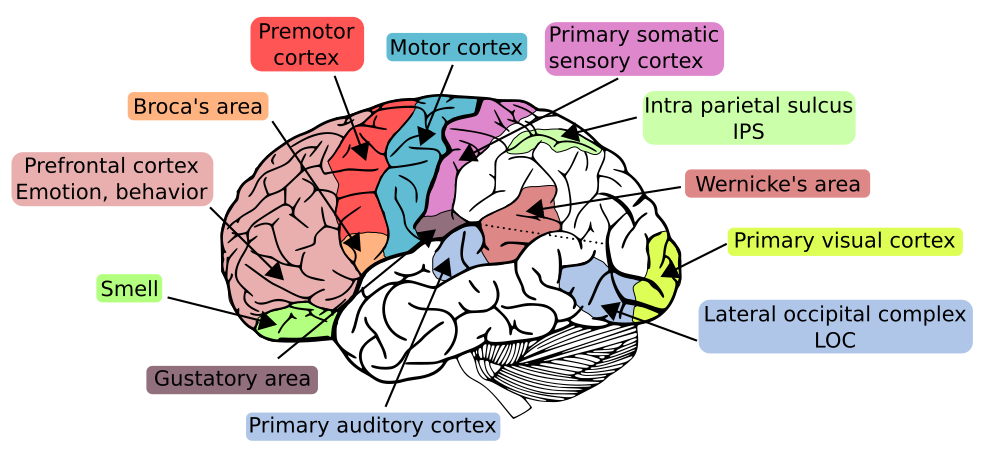
\includegraphics[width=.74\linewidth]{figures/brain_function.png}    
    \caption{\textbf{Views of the brain} at different levels of detail. The brain is composed of regions and (connected) regions are in turn composed of populations of neurons. \textbf{Left:} Simplified view of a neuron.
A \textit{neuron} has a cell body
called the \textit{soma}, many regions for receiving information from other neural cells
called \textit{dendrites}, and often an \textit{axon} (nerve
fiber) for transmitting information to other
cells (an axon can be longer than 1 meter in humans).
The information in the axon is transmitted through an electrical
signal called action potential, which is based on the electrical
properties of the neuronal membrane. Adapted from
\url{http://commons.wikimedia.org/}. \textbf{Right:}
The main functional regions of the human brain (left hemisphere).
Adapted from \url{http://agaudi.files.wordpress.com/}.}
\end{pagefigure}

\newthought{A major goal} of the neurosciences is to understand the structure, function, and variability of the human brain, and how these give rise to the complex high-level behavior patterns observed. One is typically interested in such things like:
\begin{itemize}
  \item Which parts of the brain are in-charge of processing mathematical formulae as opposed to ordinary natural language ?
  \item Which parts of the brain increase their activity when the brain is at rest ?
  \item What are the neuro-biological markers of this or that mental illness ?
  \item How does the brain structure (sulci, gyri, etc.) change during aging ? etc.
 \item How does the language network of one subject compare to that of another ? Are they alignable ?
 \item How are the different cognitive functions (language, motor, emotion, etc.) distributed over the brain, in terms of regions and networks of regions ?
 \item How are numbers represented and manipulated in the brain ?
 \end{itemize}
 The scientist might also be interested in how the brain and behavior change under the attack of an illness (e.g Schizophrenia).

Neuro-imaging has emerged as data-acquisition and analysis set of techniques of probing and observing the relevant brain systems. These go hand-in-hand with
  statistical analysis methods for analyzing them, in view of making specific quantifiable claims. These techniques operate at a scale much coarser than that of the neuron: one is interested physiological effects which are utilmately aggregates of neuronal activity over larger volumes.

  \paragraph{Organization of the chapter.} In this introductory chapter, I review the relevant theory sufficient to situate my own work in a larger scientific context. Section \ref{sec:fmri} will
  focus on imaging the brain and preprocessing of the collected data. Then follows section \ref{sec:glm} which discusses classical methodologies for analyzing the data, with a focus on the localization of task-based brain activity.
  Section \ref{sec:rsfmri} will present the another way of infering brain function,
  namely the study of background activity at rest.


\section{Functional magnetic resonance imaging}
\label{sec:fmri}
Human neuroimaging consists in acquiring ex-vivo
(non-invasively) image data from normal and
diseased human populations.
Several types of functional imaging techniques have been developed. Electro-
encephalography and magneto-encephalography measure the superficial cortical neural activity of the brain with a high temporal resolution. Functional
magnetic resonance imaging (fMRI) uses strong magnetic fields to measure
oxygen flow in the brain that correlates with its activity. This technique yields
information on brain structure, variability, and function at high
spatial resolution. Finally, invasive
techniques have been developed such as positron emission tomography that
relies on a radioactive tracer to track glucose consumption.

\begin{pagefigure}%[!htpb]
  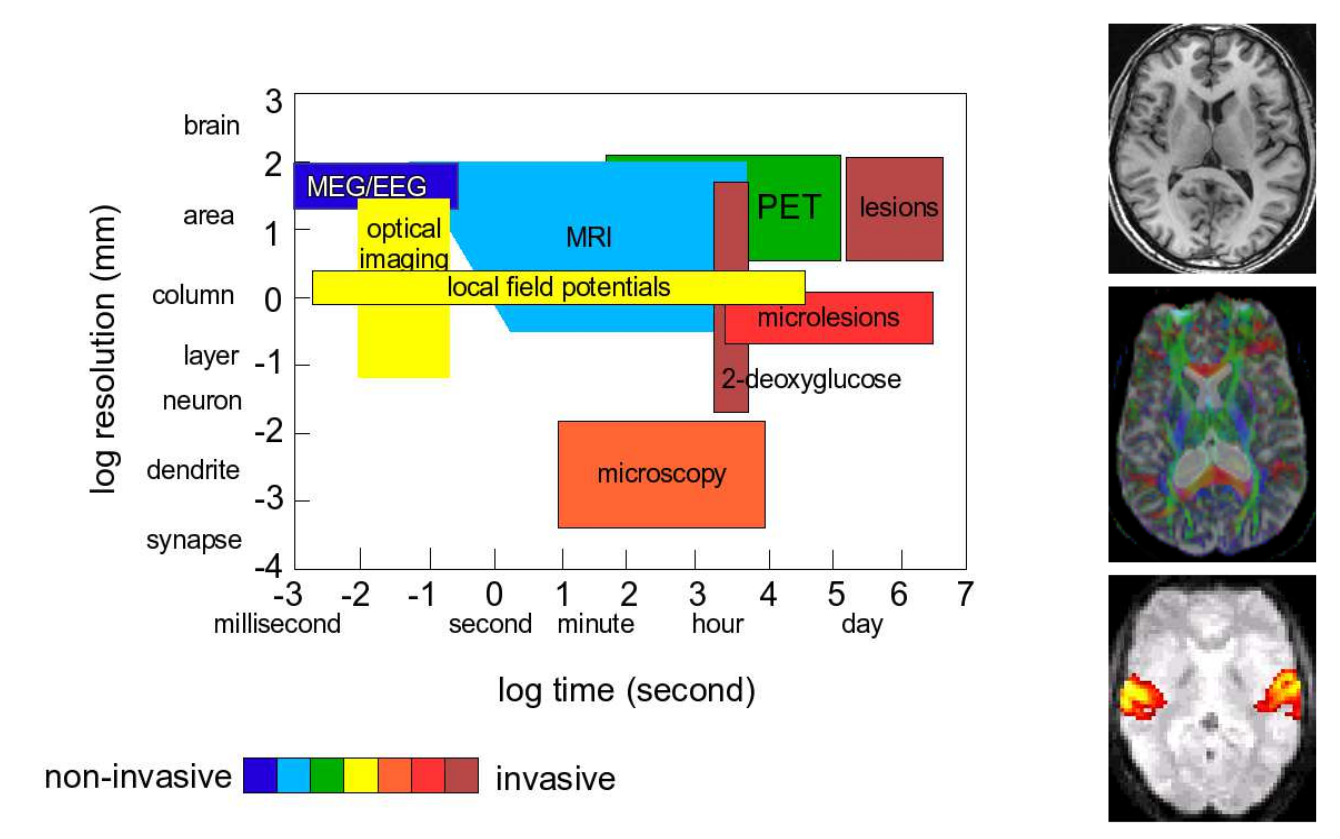
\includegraphics[width=1\linewidth]{figures/modalities.png}
  \caption{\textbf{Imaging modalities} for the brain. \textbf{Left:} The different imaging modalities for brain mapping.
      MRI and functional MRI have
the unique property to yield high-resolution information while being minimally invasive. Unlike other
modalities, MRI allows whole brain imaging. \textbf{Right:} Typical example of T1 anatomical MRI (top), pre-
processed Diffusion-Weighted (DW) MRI \textbf{middle} and fMRI \textbf{bottom} images, presented in axial views.
These images are from the Neurospin 3T scanner. For the DW-MRI image,
the main direction of water diffusion is color-coded: green for antero-posterior diffusion, red for lateral
diffusion, blue for vertical diffusion. The functional image has been analyzed to yield the regions activated
in an auditory task. Adapted with permission from~\citep{thirion_hdr}.}
\end{pagefigure}

\subsection{The BOLD signal}
When a brain area is solicited, the brain fires chemical signals to provide it
with oxygen and sugar. Nearby blood capillaries dilate to increase the quantity
of flowing blood and provide these resources. This phenomenon is called the
haemodynamic response.
As a result, we expect a higher concentration of oxygenated hemoglobin
in a given brain area soon after its activation.
fMRI imaging can be used to measured this effect, called the BOLD (\textit{Blood Oxygen-Level-Dependent}) signal, at a spatial typically resolution of 1.5 to 3mm, and a temporal resolution
of 1-3s. This yields a spatially resolved image of
brain functional networks that can be modulated
either by specic cognitive tasks or appear as
networks of correlated activity. This method is subject to several physical and physiological
noises. First,
some artifacts may be induced by radio transmitters or other equipments. Then,
spurious activations are naturally introduced by the blood vessels present in
the brain, heart beats and breathing movements. Finally, the brain can be
shifted if the subject makes large movements in the scanner.

\subsection{Preprocessing and analysis of fMRI data}
Raw fMRI images are not interpretable with bare eyes. In particular because
we are interested in small signal co-variation between voxels\footnote{Voxel stands for volume element. It refers
to a point in a 3D image, just as pixel refers to a point in a 2D image.}  and not by the
values themselves. Human eye, however, is good at perceiving global artifacts
in the data such as movements, ghost or scanner coils. Quality assessment of
preprocessed fMRI data is done by eye and by relying on dedicated medical
imaging software.. In order to prepare the data for further statistical analysis,
some preprocessing steps are required. Below, we outline the main ones. Viz,

\paragraph{Data acquisition.}
The resolution of fMRI is usually between 1mm 3 and
3mm 3 . In a single 3D scan, the brain represents $10^4$ to $10^6$ voxels.
A run contains usually from 100 to 1000 scans. Functional MRI scans are
acquired by slices, usually in the axial direction. The time required to acquire
one slice is called echo time (TE) and is in the order of tens of milliseconds.
The time required to acquire a whole 3D volume is called repetition time (TR)
and is in the order of seconds. Typical values for a 3D volume of 60 slices are
TE=33ms and TR=2s for a 3 Tesla scanner.

\paragraph{Motion-correction and coregistration to the anatomy.}
Head movement has a big impact on fMRI. A movement
with an amplitude higher than the voxel resolution (i.e. 2 to 3mm) can
shift the signal of the entire brain. Moreover, the worst impact of motion is
inflow effects, i.e. artefactual signals. In the scanner, the head of the subject is
fixed using cushion pads to avoid movements and the subject is asked to stay
as still as possible. Yet, it is impossible to completely avoid head movement.
In order to remove the effect of movement, the 3D scans are realigned on a
reference scan --usually the one in the middle of the sequence-- using rigid
body transformation (translation and rotation, without change of scale).
This is usually followed by an affine registration of the motion-corrected images to
the anatomical (T1) image of the subject, in view of subsequent inter-subject preprocessing and analysis.

\begin{figure}[!htpb]
  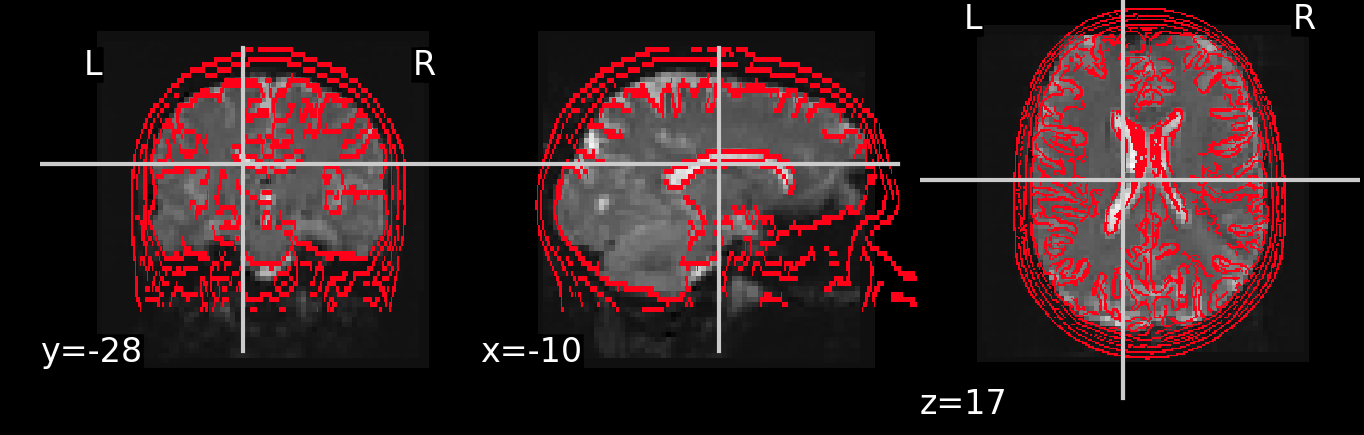
\includegraphics[width=1\linewidth]{figures/coreg.png}\\\\
  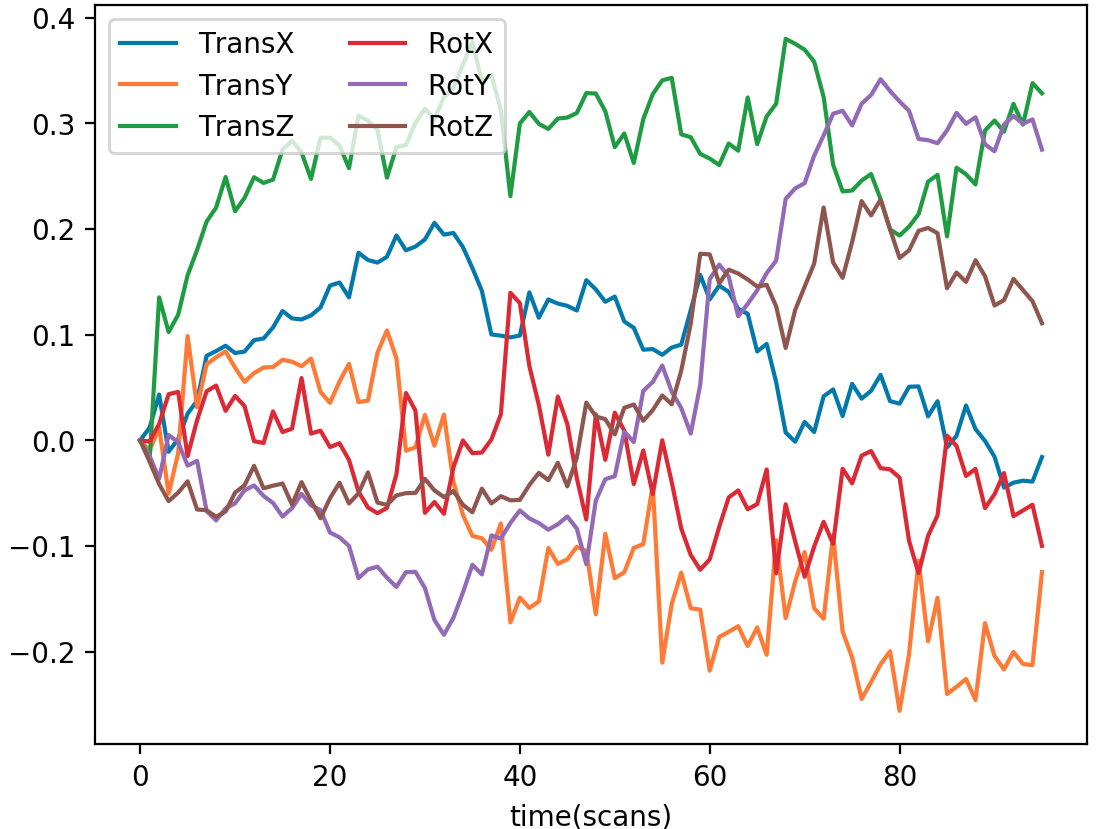
\includegraphics[width=1\linewidth]{figures/mc.png}
  \caption{\textbf{Motion-correction and coregistration.} The \textbf{top} plot shows an overlay of a subjects anatomy onto their mean functional image (the background). Here the red contours are well aligned with the background image, indicative of a successful co-registration. Typical things that can go wrong include: lesions (missing brain tissue), bad orientation headers in the images, non-brain tissue in the images (e.g skull), etc. The \textbf{bottom} plot show estimated motion parameters for the subjects-head motion. Here all movements are well below 0.5mm, which is generally considered as fine. The preprocessing and plots displayed here were done using Pypreprocess ~\url{https://github.com/neurospin/pypreprocess}, an open-source Python wrapper built on standard toolkits like SPM~\citep{friston1994statistical}.}
\end{figure}

\paragraph{Slice-timing correction.}
As stated before, brain slices are not acquired
at the same time. This introduces a shift in the haemodynamic response
associated to each of them. This problem can be solved by interpolating the
signal of each slice so that all of them can be considered as acquired at the
same time~\citep{henson1999slice}. This step is optional as, in practice, it does not bring significant
improvement. In a preliminary experiment performed on 50 individuals, we
did not observe differences in term of prediction score with or without slice
timing correction.

\paragraph{Registration of brain data into a common reference space.}
Each brain is of different size
and shape. In order to compare brain activations across several individuals, we
need to normalize them by registration to a common template~\citep{fristonbook,ashburner2005,ashburner2007,pmid19195496}. This template
can be a reference template used in the community (MNI for example). It is
also possible to compute a template directly from the data. Once a template
is chosen, for each subject, we perform two successive normalizations. First,
the anatomical scan acquired in the subject is registered to the MNI template.
Then, the fMRI data are registered to the anatomical scan. After that, the two
transformation matrices are combined in order to normalize the fMRI data to
the template. Estimation of the deformations necessary to warp a subject's brain anatomy onto a template is usually done alongside the classification of individual voxels into different classes: white matter (wm), grey matter (gm), and cerebro-spinal fluid (csf) producing so-called tissue probability maps (TPMs) ~\citep{ashburner2005}.

\begin{figure}
  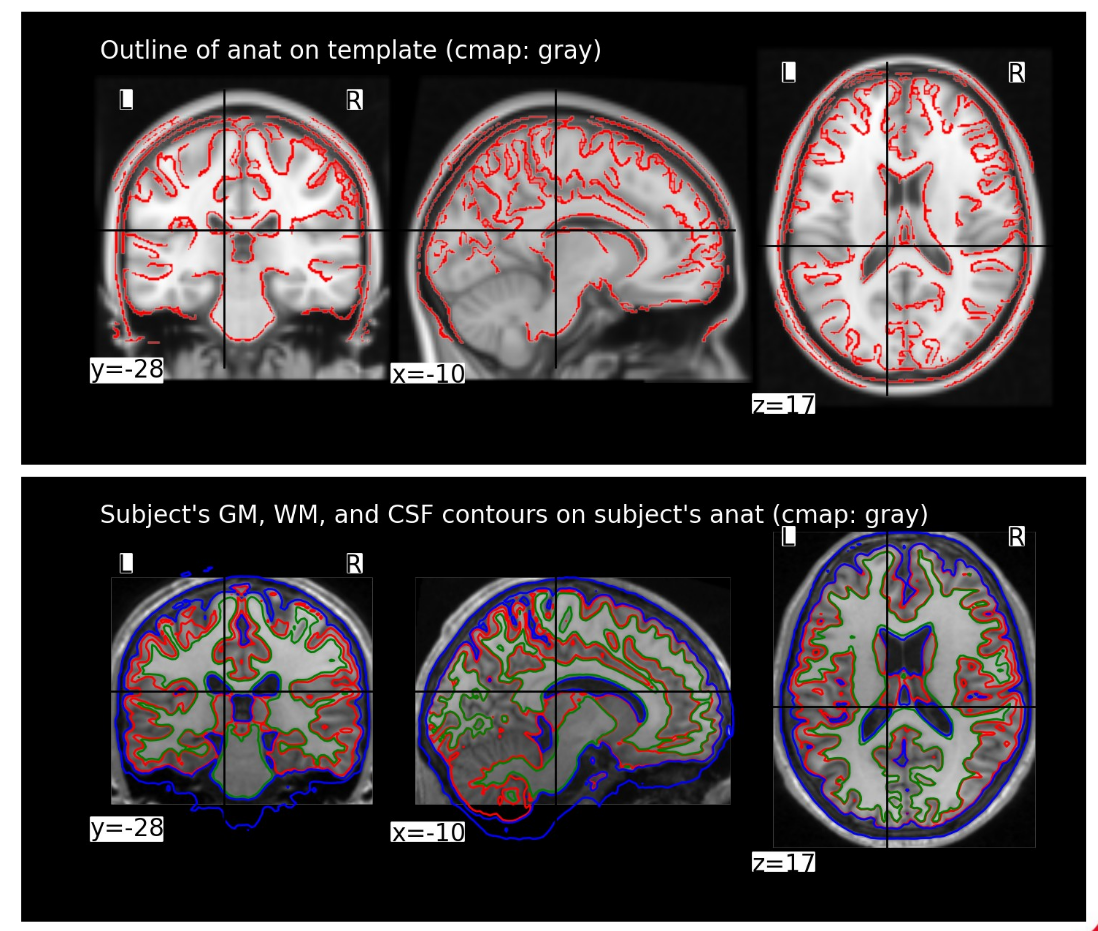
\includegraphics[width=1\linewidth]{figures/normalize.png}
  \caption{\textbf{Tissue segmentation and normalization.} Showing out the mean BOLD image of a subject and of their tissue probability maps (TPMs) after registration to a template. The contours shoud match the background image well. Otherwise, something might have gone wrong.
    Typically things that can go wrong include:
    lesions (missing brain tissue), bad orientation headers,
non-brain tissue in anatomical image (i.e needs brain
extraction), etc.}
\end{figure}

\subsection{Analysis}
\label{sec:glm}
Forward inference made on fMRI data (e.g. prediction of brain
activation from the stimuli) can be conceptualized as the encoding of perceptual,
motor or cognitive parameters into brain signals. The inverse model, that
predicts behavioral data from brain activation is called decoding. This thesis
focuses on the decoding of brain signals. Two paradigms allow to study brain
signals. Either we study them in controlled condition on a particular task,
this is the task paradigm, or we study the spontaneous activity of the brain in
order to uncover its organization, this is the resting-state paradigm.

\subsubsection{The task paradigm and the general linear model}
Using an experimental design, it is possible to relate the BOLD signal with
specific tasks performed by the subject. For example, a sound can be played in
the left or the right ear of the subject. By comparing brain activation between
resting state and when the sound is playing, we can isolate the auditory cortex
of the brain.
Statistically, we do that by crafting a design matrix corresponding to the
experiment: one column of the matrix represents one particular activation~\citep{friston1994statistical}.

\begin{figure}
  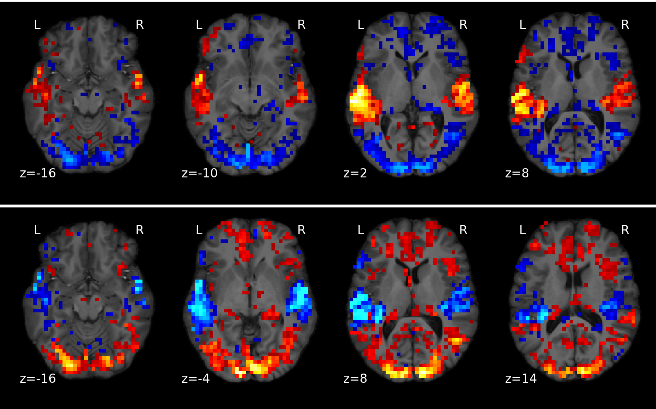
\includegraphics[width=1\linewidth]{figures/activation.png}
  \caption{\textbf{Subject-level Activation maps } for auditory versus visual and visual versus auditory conditions. Here, we show an axial via (z-coordinate) of the Z-values corresponding the size of the effect, in each voxel. Values range from -13 (light blue) to +13 (light red). Analysis was done using the \textit{Nistats} open-source Python library \url{https://github.com/nistats/nistats}.}
\end{figure}

Columns corresponding to known artifacts of the BOLD signal, such as heart
beats or movements, can be added in the design matrix in order to regress out
the part of the signal related to them. We then use a general linear model (GLM) to
recover the brain maps corresponding to each of the columns in the design
matrix $\X \in \mathbb R^{T \times k}$, where $k$ is the number of conditions and $T$ is the number of time points (times of repetition -- TR).  It is then supposed that for each voxel $v$, the measured BOLD signal $\y_v \in \mathbb R^T$ is a linear combination of the columns of $\X$, i.e of the experimental conditions, that is

\begin{equation}
  \B{y}_v = \B{X}\boldsymbol{\beta}_v + \boldsymbol{\epsilon}_v,
\end{equation}
where $\boldsymbol{\beta}_v \in \mathbb R^k$ are regression coefficients.
Such a problem is posed and least-squares is used to obtain a solution
\footnote{There are usually more time points than experimental conditions, and so problem is full-rank.},
to obtain $\hat{\boldsymbol{\beta}}_v = \B{X}^\dagger\B{y}_v$.  Stacking these coefficients across all voxels per-brain correspond to $k$ so-called $\boldsymbol{\beta}$-maps~\citep{friston1994statistical}. For a given combination of experimental conditions \footnote{For example, for $k = 3$ conditions, one may be interested in take $\B{c} = (1, -1, 0)$, meaning we wish the find the effect of the first condition relative to the second, or $\B{c}=(1,-1/2,-1/2)$ corresponding to the effect of the first condition w.r.t the average effect.\\}
$\B{c}  = (c_1,c_2,\ldots,c_k)\in \mathbb R^k$ , one can compute a statistic

\begin{equation}
\hat{t}_{v,\B{c}} := \frac{\B{c}^T\hat{\boldsymbol{\beta}}_v}{\sqrt{var(\boldsymbol{\epsilon}_v)\B{c}^T(\X^T\X)^{-1}\B{c}}}.
\end{equation}
Under the null hypothesis that the effect were are interested in is zero, i.e
\begin{equation}
  H_0: \B{c}^T\boldsymbol{\beta}_v = 0,
\end{equation}
the above statistic is student-t distributed with $T-k$ degrees of freedom, and one can do testing analytically to obtain $p$-values and confidence intervals. Projecting these values unto the brain (one value per voxel) yields a so-called \textit{activation map}. Such maps are the main output of any forward analysis in task-based fMRI studies.

One notes that $T-k$ is only a crude over-estimation of the true degrees of freedom, confounded by the fact that there are correlations between neighboring voxels, leading to \textit{multiple comparison} issues in these so-called \textit{mass-univariate} methods. Bonferoni and similar correction procedures are usually used to alleviate these issues, but maybe too conservative and destroy the the sought-for effects. An alternative is to use \textit{multi-variate} methods which directly model the spatial interactions between the voxels. Such methods will be the subject of chapter \ref{chap:structured_priors}.

\section{Resting-state fMRI, brain networks, and functional connectivity}
\label{rsfmri}
Resting state fMRI (or rsfMRI) uses the same acquisition method as task fMRI.
However, instead of giving a particular task to the subject, they are asked to let their mind wander without sleeping. By studying this background activity of
the brain, it is possible to uncover its underlying organization~\citep{raichle10}. Unlike the techniques described previously where the aim was to localize regions of activation for a given set of conditions, in functional connectivitly analysis were interested in infering connections between such regions.

Depending on the protocol, the subject can be asked to keep eyes closed or
to contemplate a fixation cross. The fixation cross prevents random eye movements
and helps the subject not to sleep.
In rsfMRI, we do not study the signal of each voxel itself but the
interactions between the brain voxels. In particular, we study the functional
connectivity of the brain, i.e. the similarity of activation patterns between
brain regions that share a common functional role. Since there is no design
matrix in rest fMRI, one must be careful to properly regress out physiological
noises or spurious correlations may appear between brain regions, in particular
longitudinally~\citep{power2012,vandijk2012}.
A first approach of functional connectivity is the voxel to voxel approach in
which the similarity is measured between each pair of voxels. This method is
not only computationally expensive, given the number of voxels in the brain,
but it is also unfounded from the statistical standpoint: it requires the estima-
tion of millions of parameters, much more than the number of observations
supports. As a consequence, some form of dimensionality reduction --a feature
selection or extraction-- is necessary to study connectivity.

% \section{Resting-state networks}
% \section{Clinical implications}
% \begin{figure}[!htbp]
%   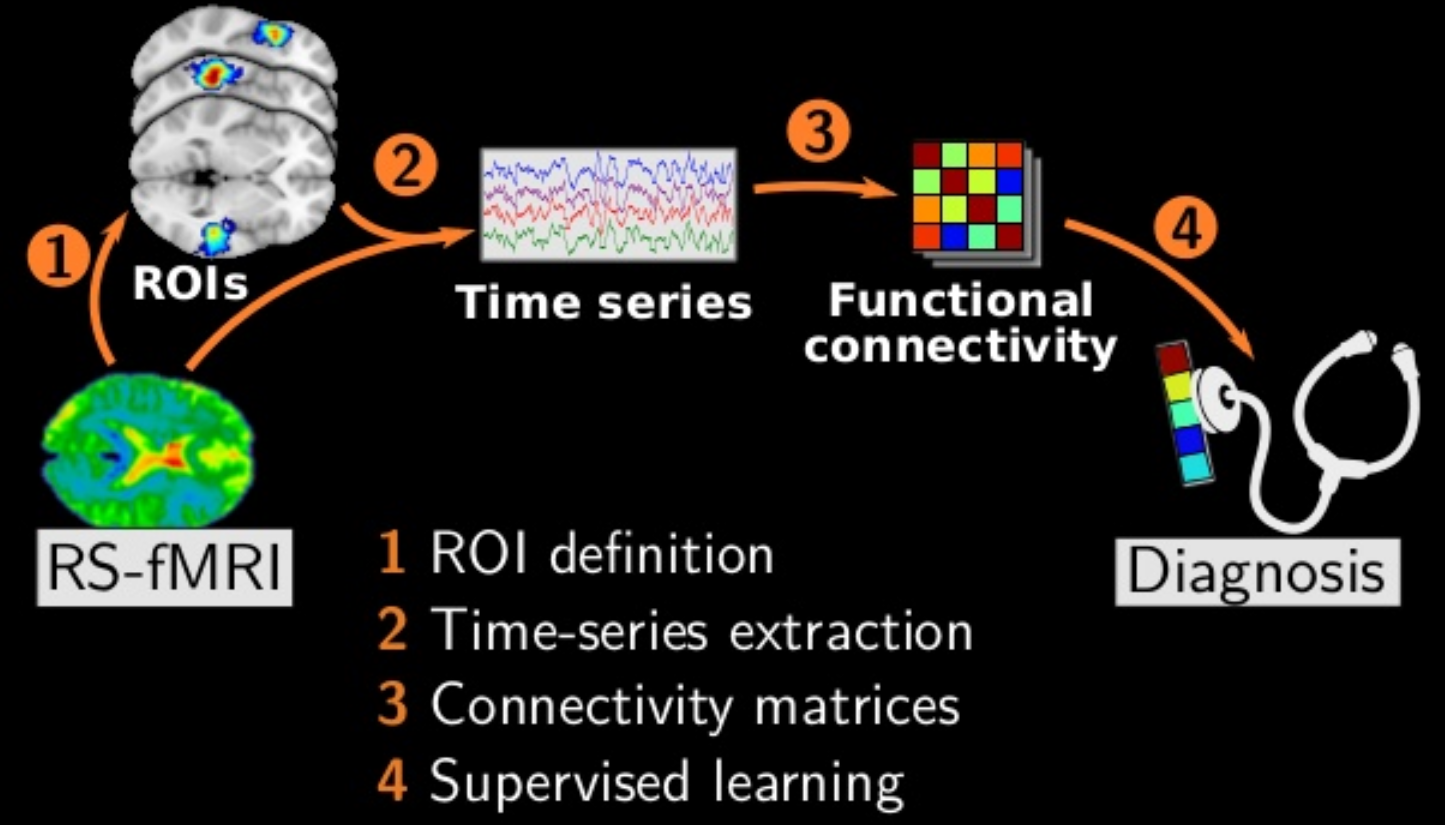
\includegraphics[width=1\linewidth]{figures/big_picture.png}
%   \caption{...}
% \end{figure}
% \section{The functional brain as a dynamic graph}
\begin{marginfigure}%[!htbp]
  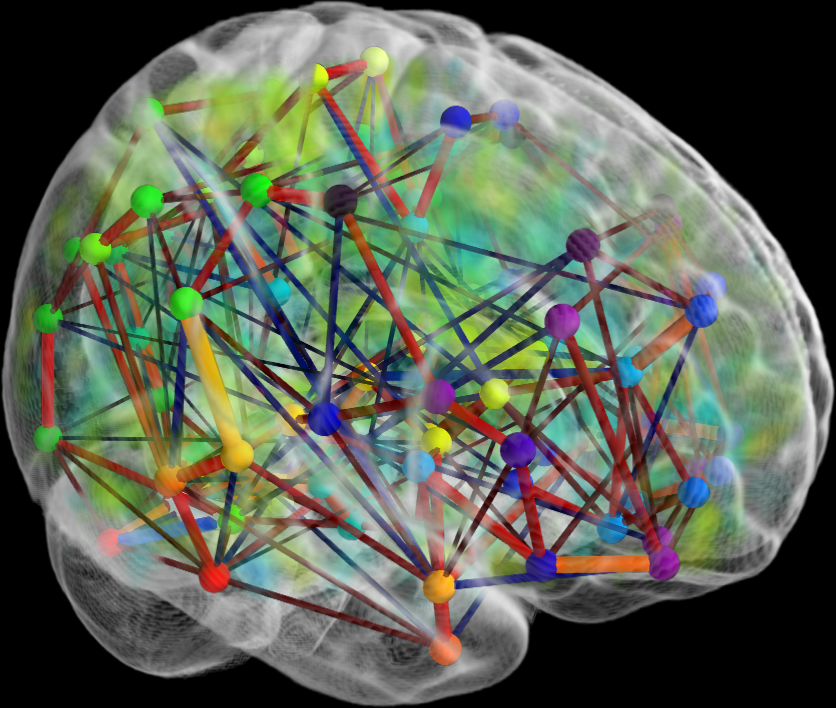
\includegraphics[width=1\linewidth]{figures/connectome.png}
  \caption{\textbf{Functional connectivity} patterns extracted from resting state data. The nodes are regions of the brain, and the thickness
  of the edges represent the relative strength average signal between the two corresponding regions.}
\end{marginfigure}

% \section{Task activation as a small perturbation of resting-state networks}

\section{Inter-subject variability in the human brain}
\subsection{Structural variability: the human brain varies in structure, size, and shape}
\subsection{Functional variability: the human brain varies in function}

  
% The first two chapters of this thesis introduce and define concepts that will be developed later on. The other chapters can be read independently of each other. Original contributions and their relative published material are referenced at the beginning of each chapter.



% % This thesis is organized in a way such that Chapter~\ref{chap:intro_fmri} and Chapter~\ref{chap:stats_fmri} are introductory chapters that define the concepts that will be developed in later chapters. The rest of the chapters only depend on these two introductory chapters and can be read independently of each other. 
%  % We propose novel extensions and investigate the theoretical properties of different models. 


% % This thesis is organized in several chapters. Chapter~\ref{chap:intro_fmri} and \ref{chap:stats_fmri} define the concepts that will be developed in later chapters. Chapter~\ref{chap:hrf_estimation} and Chapter~\ref{chap:decoding_ordinal} propose novel applications of machine learning to the analysis of fMRI. Finally, Chapter~\ref{chap:consistency}, which is the most theoretical contribution investigates 


% %Feature extraction and supervised learning on fMRI: From practice to theory

% \vspace{10pt}
% \section*{Chapter \ref{chap:intro_fmri} - Introduction to Functional MRI}

% In this chapter we introduce functional magnetic resonance imaging (fMRI) as a non-invasive functional imaging modality with good spatial resolution and whole brain coverage. We start by presenting briefly the main human brain structures and then reviewing the principal brain imaging techniques in use nowadays, with special emphasis on fMRI.

% The primary form of fMRI measures the oxygen change in blood flow. This is known as the the Blood-oxygen-level dependent (BOLD) contrast. We present a \emph{feature extraction} model known as the \emph{general linear model} (GLM)~\citep{Friston1995} that allows to extract time-independent \gls{activation coefficient}  given the BOLD signal and an experimental paradigm. The difficulty of this process stems from the fact that the BOLD signal does not increase instantaneously after the stimuli onset nor does it return to baseline immediately after the stimulus offset. Instead, the BOLD signal peaks approximately 5 seconds after stimulation, and is followed by an undershoot that lasts as long as 30 seconds. The idealized, noiseless response to an infinitesimally brief stimulus is known as the \emph{Hemodynamic Response Function} (\gls{HRF}).


%  % We describe the main assumptions behind this model: a known form of the hemodynamic response function (HRF) and the linear-time-invariant relationship between the BOLD signal and the neural response. 


% \begin{marginfigure}[-2cm]
% \centering \includegraphics[width=1.\linewidth]{figures/chapter_1/linear_hrf_mini.pdf}
% \caption{The general linear model (GLM) predicts that the expected BOLD response to two overlapping stimuli is the sum of the two independent stimuli. In green, the response to the first stimulus that is located at 1 second. In orange, the response to the second stimulus that appears at 6 seconds. In blue, the predicted BOLD response.}\label{fig:1_lti_hrf} 
% \end{marginfigure}


% % The \emph{Hemodynamic Response Function} (HRF) represents the ideal, noiseless response to an infinitesimally brief stimulus. Different versions of the HRF have been proposed in the literature and in this chapter we examine the characteristic of the HRF used in three different software packages: SPM, AFNI and NiPy.



% In order to estimate the activation coefficients, the GLM assumes a \emph{linear time invariant} (LTI) relationship between the BOLD signal and the neural response. This relationship has been reported in a number of studies and can be summarized as $i)$ \emph{Multiplicative scaling}. If a neural response is scaled by a factor of $\alpha$, then the BOLD response is also scaled by a factor of $\alpha$.
% \mbox{$ii)$ \emph{Additivity}}. If the response of two separate events is known, the signal for those same events is the sum of the independent signals (Fig.~\ref{fig:1_lti_hrf}).
% $iii)$ \emph{Time invariant}. If the stimulus is shifted by $t$ seconds, the BOLD response will also be shifted by this same amount.

% The GLM in its classical formulation assumes a known form for the hemodynamic response function (HRF). In Chapter~\ref{chap:hrf_estimation} we will present an extension of the GLM model that estimates jointly the activation coefficients and the hemodynamic response function.


% % The General Linear Model (\gls{GLM}) makes use of the knowledge of the hemodynamic response function and linear-time-invariant assumption to model the observed BOLD signal. This model states that the BOLD signal can be expressed in terms of a linear combination of the predicted fMRI responses for different stimuli (also denoted \gls{conditions}) plus a noise term (Fig.~\ref{fig:glm1_abs}). 

% % \begin{figure*}[t]
% % \center \includegraphics[width=.8\linewidth]{figures/chapter_1/glm_plain.pdf}
% % \caption{The GLM expresses the observed BOLD signal as a linear combination of regressors plus an error term. Each regressor of the design matrix is the convolution of a reference HRF and the stimulus function, a function that is 1 when the stimulus is present and zero otherwise. Each element of the (unknown) activation coefficeints represent the relative amplitude of a given condition.}\label{fig:glm1_abs}
% % \end{figure*}




% \section*{Chapter 3 - Statistical Inference in fMRI}

% In this chapter we present the statistical methods that will be used for drawing conclusions from fMRI experiments in further chapters. The chapter is divided into two sections. The first section summarizes the basics of statistical hypothesis testing while the second section describes the basics of supervised machine learning.


% Statistical tests can be broadly divided into \emph{parametric} and \emph{nonparametric} tests. Parametric test assume a known probability distribution under the null hypothesis for the distribution parameter that is under consideration. Nonparametric tests do not assume a known form of this probability distribution although they might require some regularity conditions on the distribution such as symmetry. In this chapter  we  describe two parametric statistical tests: the $t$-test and the $F$-test. We will also present a nonparametric test: the Wilcoxon signed-rank test. These tests will be used at different parts of the manuscript. The $t$ and $F$-test will be used to perform voxel-wise inference in section~\ref{subsec:spms} and the Wilcoxon test will be used to compare the performance of different supervised learning models in Chapter~\ref{chap:hrf_estimation}, \ref{chap:decoding_ordinal} and \ref{chap:consistency}.



% \begin{marginfigure}
% \center \includegraphics[width=0.8\linewidth]{chapter_2/spm_visual_auditory_mini.pdf}
% \caption{Statistical Parametric Maps (SPMs) are images with values that are, under the null hypothesis, distributed according to a known probability density function. In the figure, a $t$-map (i.e. the values are distributed according to a Student $t$ distribution) for a contrast of a Visual vs an Auditory task. Thresholded at $p$-value $< 10 ^ {-3}$. It can be seen how the voxels that exhibit a higher significance of this contrast belong to visual areas (red) and auditory areas (blue)}\label{fig:abs_spm}
% \end{marginfigure}

% A notable application of parametric statistical tests to fMRI is the creation of Statistical Parametric Maps (SPMs) (Fig.~\ref{fig:abs_spm}). These are images with values that are, under the null hypothesis, distributed according to a known probability density function, usually Student $t$ or the $F$ distribution. To create such maps, one proceeds by performing a parametric test at each voxel. The resulting statistics are assembled into an image - the SPM. 



% In the second part of this chapter we introduce different supervised learning models that will be used in subsequent chapters. We will consider models that can be estimated as the solution to a minimization problem of the form
% $$
% \argmin_{f \in \mathcal{F}} {\mathcal{R}}_n^{\psi}(f) + \lambda \Omega(f) \quad,
% $$
% where $\mathcal{R}_n^{\psi}(f)$ is a data-fitting term that minimizes a surrogate of the loss function term and $\Omega(f)$ is a regularization term that biases the estimated model towards a set of desired solutions. This way, the model is a trade-off between a data fidelity term and a regularization term. 

% We describe different surrogate loss functions and penalties that have found applications in the context of fMRI analysis. The surrogate loss functions that we describe here are Support Vector Machines, Logistic Regression, Support Vector Regression and Least Squares. The penalties that we consider here are squared $\ell_2$, $\ell_1$, elastic-net ($\ell_2^2 + \ell_1$) and total-variation (TV).



% Finally, we present two applications of supervised learning to reveal cognitive mechanisms in fMRI studies. The first application is commonly known as \emph{decoding} or \emph{mind reading} and consist in predicting the cognitive state of a subject from the activation coefficients. The neuroscientific questions that decoding is able to address are commonly shaped within the statistical hypothesis testing framework. The inference that we want to establish is whether the classifier trained on data from a given brain area of one subject is accurate enough to claim that the area encodes some information about the stimuli. In this setting, the null hypothesis is that a given brain area does not contain stimuli-related information. The ability of the classifier to correctly predict some information about the stimuli is considered a positive evidence in support of the alternate hypothesis of presence of stimuli-related information within the brain activity. As an application of decoding, we present the dataset~\citep{Borghesani2014}, in which we used decoding techniques to establish in which regions of the brain it is possible to decode different aspects of words representing real-world objects.


% A different application is known as \emph{encoding}. Here, the activation coefficients are predicted from some information about the stimuli. The success of an encoding model depends in great measure on our ability to construct an appropriate representation of the stimuli, a transformation that is often nonlinear. For example, \citet{naselaris2009bayesian} constructed two different models for each voxel: a model based on phase-invariant Gabor wavelets, and a semantic model that was based on a scene category label for each natural scene. The authors showed that the Gabor wavelet model provided good predictions of activity in early visual areas, while the semantic model predicted activity at higher stages of visual processing. 


% Encoding and decoding can be seen as complementary operations: while encoding uses stimuli to predict activity,  decoding uses activity to predict information about the stimuli. Furthermore, encoding offers the advantage over decoding models that they can naturally cope with unseen stimuli. For example, \citep{Kay2008} used an encoding model to identify natural images that the subject had not seen before. In this case, the predicted activation coefficients were used to select the image that matched most closely the measured activation coefficients.



% \begin{fullwidth}
% \section*{Chapter~\ref{chap:hrf_estimation} - Data-driven HRF estimation for encoding and decoding models}
% \end{fullwidth}


% % In this chapter we describe a novel method for the simultaneous estimation of HRF and activation coefficients based on low-rank modeling, forcing the estimated HRF to be equal across events or experimental conditions,
% %  yet permitting it to differ across voxels. Estimation of this model leads to
% % an optimization problem that we propose to solve with using a
% % \mbox{quasi-Newton} method, exploiting fast gradient computations. 
% % We compare 10 different HRF modeling methods in terms of encoding and decoding
% % score on two different datasets. These results show that the \mbox{R1-GLM} model
% % outperforms competing methods in both encoding and decoding
% % settings, positioning it as an attractive method both from the points of view
% % of accuracy and computational efficiency.


% As pointed in Chapter~\ref{chap:intro_fmri}, prior to its use statistical inference procedures, the fMRI data usually goes through \emph{feature extraction} process that converts the BOLD time course into time-independent \gls{activation coefficient}. This is commonly achieved using a model known as Linear General Model (GLM). While
% this approach has been successfully used in a wide range of studies, it does
% suffer from limitations. For instance, the GLM commonly
% relies on a \mbox{data-independent} \emph{reference} form of the hemodynamic response function
% (HRF) to estimate the activation coefficient (also known as \emph{canonical} or \emph{reference} HRF). However it is
% known that the shape of this response function
% can vary substantially across subjects, age and brain regions. This suggests that an adaptive modeling of this
%  response function can improve the accuracy of subsequent analysis.



% % At a given voxel, it is expected that for similar stimuli the estimated HRF are also 
% % similar. Hence, a natural idea is to promote a common HRF
% % across the various stimuli (given that they are sufficiently similar), which should result in more robust estimates.
% In this work we propose a model in which a common HRF is shared
% across the different stimuli that we denote \emph{Rank-1 GLM} (R1-GLM). The novelty of our method stems from the observation that the formulation of the GLM  with a
% common HRF across conditions translates to a rank constraint on the vector of estimates. 
% This assumption amounts to enforcing the vector of
% estimates to be of the form $\bfbeta_{\B{B}} = [\mathbf{h} {\beta}_1, \mathbf{h} \beta_2, \cdots, \mathbf{h}
% \beta_k]$ for some HRF $\mathbf{h} \in \RR^d$ and a vector of coefficients $\bfbeta \in \RR^k$. More compactly, this can be written as $\bfbeta_{\B{B}} = \vecop(\B{h}
% \bfbeta^T)$. This can be
% seen as a constraint on the vector of coefficients to be the vectorization of a rank-one
% matrix, hence the name {\it Rank-1 GLM (R1-GLM)}.

% In this model, the coefficients have no longer a closed form expression,
% but can be estimated by minimizing the following loss function. Given $\B{X}_{\B{B}}$ and $\B{y}$ as before, $\B{Z} \in \RR^{n \times q}$ a matrix of nuisance parameters such as drift regressors, the optimization problem reads:
% %
% \begin{eqnarray}\label{eq:abs_r1}
% \begin{aligned}
% \hat{\B{h}}, ~\hat{\bfbeta},~ \hat{\bfomega} ~=~& \argmin_{\B{h}, \bfbeta, {\bfomega}} ~ \frac{1}{2}\|\mathbf{y} - \mathbf{X}_{\B{B}} \vecop(\B{h} \bfbeta^T) - \B{Z} {\bfomega}\| ^2\\
% &\text{subject to } \|\B{B} \B{h}\|_{\infty} = 1 \text{ and } \langle \B{B} \B{h}, \B{h}_{\text{ref}}\rangle > 0 \enspace ,
% \end{aligned}
% \end{eqnarray}

% \begin{figure}[t] \centering
% \includegraphics[width=.9\linewidth]{chapter_3/scores_recovery_1.pdf}
% \includegraphics[width=.9\linewidth]{chapter_3/scores_recovery_2.pdf}
% \includegraphics[width=\linewidth]{chapter_3/scores_decoding_smaller.pdf}
% \caption{\label{fig:abs_identification_scores} Image identification score (higher is better) on two different subjects from the first dataset and average decoding score on the second dataset. In the first dataset the metric counts the number of correctly identified images over the total number of images (chance level is 1/120 $\approx 0.008$). This metric is less sensitive to the shape of the HRF than the voxel-wise encoding score. The benefits range from 0.9\% points to 8.2\% points across R1-constrained methods and subjects. The highest score is achieved by a R1-GLM method with a FIR basis set for subject 1 and by a R1-GLMS with FIR basis for subject 2.

% The metric in the second dataset (decoding task) is Kendall tau. Methods that perform constrained HRF estimation significantly outperform 
% methods that use a fixed (reference) HRF. In particular,
% the best performing method is the R1-GLM with 3HRF basis, followed by the R1-GLMS with 3HRF basis. 
% }
% \end{figure}

% %
% The norm constraint is added to avoid the scale ambiguity between $\B{h}$ and $\bfbeta$
% and the sign is chosen so that the estimated HRF correlates
% positively with a given reference HRF $\B{h}_{\text{ref}}$.
% This ensures the identifiability of the parameters. The optimization problem (Eq.~\eqref{eq:abs_r1}) 
% is {\it smooth} and is convex with respect to $\B{h}$, $\bfbeta$ and $\bfomega$,
%  however it is not {\it jointly convex} in variables $\B{h}$, $\bfbeta$ and $\bfomega$.



% We compare different methods for the joint estimation of HRF and activation coefficients in terms of their score for an encoding and an encoding task. The
% methods we considered are standard GLM (denoted \gls{GLM}), a variant of the GLM that improves estimation in highly correlated settings known as GLM with separate designs (GLMS), Rank-1 GLM (R1-GLM) and Rank-1 GLM with separate designs
% (R1-GLMS). For all these models we consider different basis sets for
% estimating the HRF: a set of three elements formed by the reference HRF and
% its time and dispersion derivative, a FIR basis set (of size 20 in the
% first dataset and of size 10 in the second dataset) formed by the canonical vectors
% and the single basis set formed by the reference HRF (denoted ``fixed HRF''), which
% in this case is the HRF used by the SPM 8 software.

% We consider two different datasets. The first dataset is presented in~\citep{Kay2008} where it is investigated using an encoding paradigm. The second dataset has been presented in~\citep{Jimura_Poldrack_2011} and is naturally investigated using a decoding paradigm. The scores obtained in both datasets can be seen in Figure~\ref{fig:abs_identification_scores}. In both cases, the proposed method (R1-GLM or its variant R1-GLMS) achieve the highest scores. The results presented in this chapter have been published in~\citep{pedregosa:hal-00952554}.





% \vspace{10pt}
% \section*{Chapter~\ref{chap:decoding_ordinal} - Decoding with Ordinal Labels}

% We have presented in Chapter~\ref{chap:stats_fmri} the decoding problem in fMRI. In this setting it is often the case that the target variable consist of discretely ordered values. This occurs for example when target values consists of human generated ratings, such as values on a Likert scale, size of objects (Fig.~\ref{fig:mini_vb}), the symptoms of a physical disease or a rating scale for clinical pain measurement.


% \begin{figure}
% \includegraphics[width=\linewidth]{chapter_4/experiment.png}
% \caption{In \citep{Borghesani2014}, the authors investigated the possibility to predict different aspects of the words subjects were reading while undergoing an fMRI acquisition. One of the problems we investigated is to predict the size of the objects that the words refer to. In this case, the different stimuli are ordered according to their relative size, i.e. hammer is smaller than cow which is smaller than a whale, etc. In this case, the target variable is of \emph{ordinal nature}. }\label{fig:mini_vb}
% \end{figure}


% In this chapter we propose the usage of two loss functions to assess the performance of a decoding model when the target consist of discretely ordered values: the absolute error and pairwise disagreement. These two loss functions emphasize different aspects of the problem: while the absolute error gives a measure of the distance between the predicted label and the true label, the pairwise disagreement gives a measure of correct ordering of the predicted labels. These loss functions lead to two different supervised learning problems. The problem in which we seek to predict a label as close as possible to the correct label is known as \emph{ordinal regression} while the problem of predicting ordering as close as possible to the true ordering of a sequence of labels is traditionally known as \emph{ranking}.  

% The first models specifically tailored for the problem of ordinal regression date back to the proportional odds and proportional hazards models of~\citep{McCullagh1980}. We present three different surrogate loss functions of the absolute error: least absolute error, ordinal logistic regression and cost-sensitive multiclass classification.


% Ranking models were introduced chronologically later than ordinal regression but its popularity has grown in recent years thanks to its applicability to information retrieval (and search engines in particular)~\citep{liu2009learning}. To the best of my knowledge, the first attempt to minimize a convex surrogate of the pairwise disagreement appears is due to~\citet{Herbrich2000}. We consider a model that minimizes a surrogate of the pairwise disagreement: the RankLogistic model. This model can be viewed as a modification of the popular RankSVM model~\citep{Herbrich2000,Joachims2002}.

% The choice of either metric (absolute error or pairwise disagreement) will depend on the problem at hand. For example, in clinical applications it is often desirable to predict a label as close as possible to the true label, in which case the absolute error is the appropriate metric. If however, the purpose of the decoding study is to perform a statistical hypothesis test to claim that the area encodes some information about the stimuli, then the pairwise disagreement can be an appropriate measure~\citep{pedregosa2012learning, Borghesani2014, bekhti:hal-01032909}.




% % We examine the generalization performance of the presented models on both synthetic data and three fMRI decoding problems from two datasets. We conclude that the best performing models is the last absolute error and ordinal logistic when considering the absolute error as metric and the RankLogistic model when considering the pairwise disagreement as metric. 


% \begin{figure*}[t]
% \includegraphics[width=\linewidth]{chapter_4/scores_ordinal.pdf}
% \caption[-4cm]{Generalization errors (lower is better) for three fMRI decoding problems. Two different metrics are used corresponding to the rows in the figure: mean absolute error and mean pairwise disagreement. The $*$ symbol represents the $p$-value associated with a Wilcoxon signed-rank test. This test is used to determine whether a given method outperforms significantly the next best-performing method.}\label{fig:abs_scores_ordinal}
% \end{figure*}

% We examine their generalization error on both synthetic and two real world fMRI datasets and identify the best methods for each evaluation metric (Fig.~\ref{fig:abs_scores_ordinal}). Our results show that when considering the absolute error as evaluation metric, the least absolute error and the logistic ordinal model are the best performing methods. On the other hand, when considering the mean pairwise disagreement the RankLogistic was the best performing method. For neuroimaging studies, this contribution outlines what in our opinion are the best models to choose when faced with a decoding problem in which the target variables are naturally ordered.




% \section*{Chapter~\ref{chap:consistency} - Fisher Consistency of Ordinal Regression \mbox{Methods}}


% Ordinal regression is the supervised learning problem of learning a rule to predict labels from an ordinal scale. Some ordinal regression models have been  used in Chapter~\ref{chap:decoding_ordinal} to model the decoding problem when the target variable consist of ordered values.

% Motivated by its applicability to decoding studies we turn to study some theoretical properties of these methods. The aim is that a theoretical approach can provide a better understanding the methods at hand. For example, \citet{Keerthi2003} proposed two different models for the task of ordinal regression: SVOR with explicit constraints and SVOR with implicit constraints. In that work, the second approach obtained better generalization error in terms of the absolute error loss function. Similar results were obtained by~\citet{lin2006large} replacing the hinge loss by an exponential loss. Yet again, \citet{Rennie} arrived to similar conclusions considering the logistic loss instead. Given these results, it seems natural to ask: is this coincidence or are there theoretical reasons for  this behavior? We will use the result of this chapter to provide an affirmative answer to this last question.
% % By the end of the chapter we will be able to affirmatively answer this question.

% Many of the ordinal regression models that have been proposed in the literature can be viewed as methods that minimize a convex surrogate of the zero-one, absolute (as outlined in Chapter~\ref{chap:decoding_ordinal}), or squared errors. In this chapter we investigate some theoretical properties of ordinal regression methods. The property that we will investigate is known as \emph{Fisher consistency} and relates the minimization of a given loss to the minimization of its surrogate. 

% We consider a rich family of loss functions for ordinal regression. We follow~\citep{Li2007} and determine as admissible loss functions of ordinal regression those that verify the V-shape property, a condition that includes to the best of my knowledge all popular loss functions that have been used in the context of ordinal regression: absolute error, squared error and 0-1 loss. 

% In order to introduce the notion of consistency we must fix some notation. In the supervised learning setting, we are given a set of $n$ observations $\{(X_1,
% Y_1), \ldots, (X_n, Y_n) \}$ drawn i.i.d.~from $X\times Y$ and a \emph{loss
% function} $\ell: \mathcal{Y} \times \mathcal{Y} \rightarrow [0, \infty)$. The goal is to learn from the training examples a measurable mapping called a~\emph{classifier} $h: \XX \rightarrow \mathcal{Y}$ so that the \emph{risk} given below is as small as possible:
% \begin{equation}
% \label{eq:abs_l_risk}
% \mathcal{R}_{\ell}(h) = \EE_{X \times Y}(\ell(Y, h(X)))\quad.
% \end{equation}


% Attempting to directly minimize the risk is not feasible in practice. First, the probability distribution $P$ is unknown and the risk must be minimized approximately based on the observations. Second, due to the non-convexity and discontinuity of $\ell$, the risk is difficult to optimize and can lead to an NP-hard problem. It is therefore common to approximate $\ell$ by a function $\psi: \mathcal{Y} \times \RR^d \to \RR$, called a \emph{surrogate loss function}, which has better computational properties. The goal becomes to find the \emph{decision function} $f$ that minimizes instead the $\psi$-risk, defined as
% \begin{equation}
% \Rpsi(f) = \EE_{X \times Y}(\psi(Y, f(X))) \enspace.
% \end{equation}



% Fisher consistency is a desirable property for surrogate loss functions. It implies that in the population setting, i.e., if the probability distribution $P$ were available, then optimization of the $\psi$-risk would yield a function (not necessarily unique) with smallest possible risk, known as \emph{Bayes predictor} and denoted by $h^*$. This implies that within the population setting, the minimization of the $\psi$-risk and the minimization of the risk both yield solutions with same risk. 
% % In other words, consistency implies that the minimization of the $\psi$-risk, which is usually a convex optimization problem and hence easier to solve converges to a solution with minimal $\ell$-risk.

% \begin{marginfigure}
% \center\textbf{\color{msblue} 0-1 Error}
% \includegraphics[width=1.1\linewidth]{chapter_5/probas_or_01.pdf}
% \vspace{-30pt}\center\textbf{\color{msblue} Absolute Error}
% \includegraphics[width=1.1\linewidth]{chapter_5/probas_or.pdf}
% \vspace{-30pt}\center\textbf{\color{msblue} Squared Error}
% \includegraphics[width=1.1\linewidth]{chapter_5/probas_or2.pdf}
% \caption{
% 	Bayes predictor can be visualized on the probability simplex. Bayes predictor is a function of the conditional probability $\eta_i(x) = P(y\!=i|X\!=\!x)$. The vector $(\eta_1, \ldots, \eta_k)$ belongs to the probability simplex of $R^n$, which is contained within an hyperplane of dimension $k-1$. In the figure, probability simplex in $\RR^3$ is colored according to the output of Bayes predictor.
% }\label{fig:bayes_predictor}
% \end{marginfigure}



% In this chapter we provide a theoretical analysis of the Fisher consistency properties of a rich family of ordinal regression surrogate loss functions, including proportional odds and support vector ordinal regression. The loss functions that we considered can be divided into three categories: regression-based, threshold-based and classification-based. 


% \paragraph{Regression-based loss function. }The \emph{\mbox{regression-based approach}} treats the labels as real values. It uses a standard regression algorithm to learn a real-valued function, and then predicts by rounding to the closest label. In this setting we will examine consistency of two different surrogate loss functions, the absolute error (that we will denote $\psi_{\mathcal{A}}$) and the squared error (denoted $\psi_{\mathcal{S}}$), which are convex surrogates of $\ell_{\mathcal{A}}$ and $\ell_{\mathcal{S}}$, respectively. Given $\alpha \in \RR$, $y \in [k]$, these are defined as
% \begin{equation*}
% \psi_{\mathcal{A}}(y, \alpha) = |y - \alpha|, \quad \psi_{\mathcal{S}}(y, \alpha) = (y - \alpha)^2 \quad.
% \end{equation*}

% We prove that the $\psi_{\mathcal{A}}$ surrogate is consistent with respect to the absolute error and that the $\psi_{\mathcal{S}}$ surrogate is consistent with respect to the squared error. Consistency of $\psi_{\mathcal{A}}$ was already proven by~\citep{Ramaswamy2012} for the case of 3 classes. Here we give an alternate simple proof that extends beyond $k>3$. 

% \paragraph{\bf Threshold-based loss function.} While the regression-based loss functions may lead to optimal predictors when no constraint is placed on the regressor function space as we will see, in practice only simple function spaces are explored such as linear or polynomial functions. In these situations, the regression-based approach might lack flexibility. \emph{\mbox{Threshold-based} loss functions} provide greater flexibility by seeking for both a mapping $f: \XX \to \RR$ and a non-decreasing vector $\btheta \in \RR^{k-1}$, often referred to as~\emph{thresholds}, that map the class labels into ordered real values. In this context of we consider two different families of surrogate loss functions: the \emph{cumulative link} surrogates and the \emph{margin-based} surrogates. The first family of surrogate loss function that we will consider is the \emph{cumulative link} surrogates. In such models the posterior probability is modeled as $P(Y \leq i|X\!=\!x) = \sigma(g_i(x))$, where $\sigma$ is an appropriate link function. We will prove consistency for the case where $\sigma$ is the sigmoid function, i.e., $\sigma(t) = 1/(1 + \exp(-t))$. This model is known as the \emph{proportional odds} model or \emph{cumulative logit} model~\citep{McCullagh1980}. For $x \in \XX, y \in [k]$ and $\alpha_i = g_i(x)$, the proportional odds surrogate (denoted $\psi_{\mathcal{C}}$) is defined as
% \begin{equation}\label{eq:propodds}
% \psi_{\mathcal{C}}(y, \balpha) = 
% \begin{cases}
% -\log(\sigma(\alpha_1)) &\text{ if } y = 1 \\
% -\log(\sigma(\alpha_y) - \sigma(\alpha_{y-1})) &\text{ if } 1 < y < k \\
% -\log(1 - \sigma(\alpha_{k-1})) &\text{ if } y = k.
% \end{cases}
% \end{equation}
% The other family of surrogates, the margin-based surrogates (denoted $\psi^{\ell}_{\mathcal{M}}$) depends on a V-shaped loss function $\ell$ and is given by
% \begin{gather*}
% \label{eq:sum_of_loss}
% \psi^{\ell}_{\mathcal{M}}(y, \balpha) =
% \sum_{i = 1}^{y-1} \Delta \ell(y, i)\phi(\alpha_i) - \sum_{i=y}^{k-1}\Delta \ell(y, i)\phi(-\alpha_i) \enspace.
% \end{gather*}
% where $\Delta\ell(y, i)$ is the forward difference with respect to the second parameter, defined as $\Delta\ell(y, i) = \ell(y,i+1) - \ell(y, i)$. This formulation parametrizes several popular approaches to ordinal regression. For example, let $\phi$ be the hinge loss and $\ell$ the zero-one loss, then $\psi^{T}_{\ell}$ coincides with the Support Vector Ordinal Regression (``explicit constraints'' variant) of~\citep{Shashua, Chu2007}. If instead the mean absolute loss is considered, this approach coincides with the ``implicit constraints'' formulation of the same reference. For other values of $\phi$ and $\ell$ this loss includes the approaches proposed in~\citep{Shashua,Keerthi2003,Rennie,lin2006large}.

% % Since consistency of the threshold-based approach is only proven subject to certain conditions on the underlying probability distribution $P$, we  investigate which are the conditions that guarantee consistency of these surrogates.

% \paragraph{\bf Classification-based loss function} Since we aim at predicting a finite number of labels with a specific loss functions, it is also possible to use generic multiclass formulations such as the one proposed in~\citep{lee2004multicategory} which can take into account generic losses. Given $\phi$ a real-valued function, this formulations considers the following surrogate
% \begin{equation} \label{eq:multiclass}
% \psi_{\mathcal{L}}^{\ell}(y, \balpha) = \sum_{i=1}^k \ell(y, i) \phi(-\alpha_i)
% \end{equation}
% for $\balpha \in \RR^k$ such that $\sum_{i=1}^k \alpha_i = 0$. The prediction function in this case is given by ${\rm pred}(\balpha) = \argmax_{i \in [k]} \alpha_i$. Note however that this method requires the estimation of $k-1$ decision functions. For this reason, in practical settings threshold-based are often preferred as these only require the estimation of one decision function and $k-1$ thresholds.Consistency results of this surrogate was proven by~\citet{Zhang}, so we will limit ourselves to compare their results to our findings of consistency for threshold-based surrogates in Section~\ref{subsec:multiclass}.





% For all the surrogates considered, we either prove consistency or provide sufficient conditions under which these approaches are consistent. Finally, we illustrate our findings by comparing the performance of two methods on 8 different datasets. Although the conditions for consistency that are required by the underlying probability distribution are not necessarily met, we observed that methods that are consistent w.r.t a given loss often outperform other methods that are not consistent with respect to that loss.




% \section*{Chapter \ref{chap:conclusion} - Conclusion and Perspectives}

% We summarize the contributions of this thesis and point out possible extensions that can be considered in the future. These are:

% \begin{enumerate}
% \item For the R1-GLM model introduced in Chapter~\ref{chap:hrf_estimation} we outline a possible direction to improve its computational properties by means of tensor factorizations. 

% \item For the R1-GLM we outline an approach to consider a common HRF at the parcel level. This would allow the model to take advantage of the spatially dependent nature of fMRI. 

% \item The R1-GLM model, being non-convex, comes with no guarantees of convergence to a global optimum for the algorithms considered. We propose to study conditions under which the model is guaranteed to have a unique global optimum.


% \item Some of the results presented in Chapter~\ref{chap:consistency} are valid under restrictive conditions on the probability distribution that generates the data. We propose to extend these results to a more general setting by relaxing some of the conditions imposed to achieve consistency of some models.

% \item We report the possibility to apply ordinal regression methods to 0-1 multiclass classification. Although ordinal regression methods have been initially developed for loss functions that minimize a distance between the labels (typically the absolute error loss), our theoretical results show that some popular models are instead consistent with the 0-1 loss. This suggest that these methods might be competitive within a multiclass classification setting. A potential advantage of these methods compared to other multiclass classification methods is the lower amount of parameters to estimate.
% \end{enumerate}




% % Afin d'estimer les coefficients d'activation, le GLM suppose une relation linéaire invariant de temps (LTI) entre le signal BOLD et la réponse neurale. Cette relation a été rapporté dans un certain nombre d'études et peut être résumée comme i) mise à l'échelle multiplicatif. Si une réponse neurale est réduite par un facteur de α, alors la réponse BOLD est également mis à l'échelle par un facteur de α. ii) d'additivité. Si la réponse à deux événements distincts est connu, le signal de ces événements se ils devaient se produire à proximité dans le temps est la somme des signaux indépendants (Fig. 2.1). iii) Durée invariant. Si le stimulus est décalée de t secondes, la réponse BOLD sera également décalé de ce même montant.
% % Le GLM dans sa formulation classique prend une forme connue pour la fonction de réponse hémodynamique (FRH). Dans le chapitre 5, nous allons présenter une extension du modèle GLM qui estime conjointement les coefficients d'activation et la fonction de réponse hémodynamique.



% \clearpage
\bibliographystyle{plainnat}
\bibliography{bib_all}


% \part{Structured priors for analyzing brain data}
\chapter{Structured priors for brain decoding and functional segmentation: the models}\label{chap:structured_priors}
\markright{{~{\rm \ref{chap:structured_priors}}. Structured priors for analyzing brain data}\hfill}{}

\minitoc

\section{Introduction to brain decoding}
As already discussed in chapter \ref{chap:bigpic}, functional brain imaging provides a distinctive opportunity to study brain functional architecture, while being minimally invasive, and is thus well-suited for the challenging study of the spatial layout of neural coding. Different modalities exist, each one having specific spatial and temporal resolutions; among them Functional Magnetic Resonance Imaging (fMRI)~\citep{agawa1990,ogawa1990b} has emerged as a fundamental modality for brain imaging, striking a good balance between spatial and temporal resolution.  fMRI images are pre-processed, and modeled through a general linear model (GLM), that takes into account the different experimental conditions and the dynamics of the haemodynamic response in the design matrix. The resulting model parameters, a.k.a. activation maps, represent the influence of the different experimental conditions on local fMRI signals.

\paragraph{The standard approach.}
The standard approach used for analyzing these activation maps is called classical inference, and relies on a mass-univariate statistical tests (one for each voxel), yielding the so-called statistical parametric maps (SPMs)~\citep{friston1994statistical}. Such maps are of particular interest in cognitive neuroscience, as they open the door to localizing the voxels that are significantly active for any combination of experimental conditions, and thus are probably implied in the underlying neural code of the cognitive processes. However, this classical inference suffers from multiple comparisons issues. Also, it does not take into account the multivariate structure of the fMRI data.

\begin{pagefigure}
  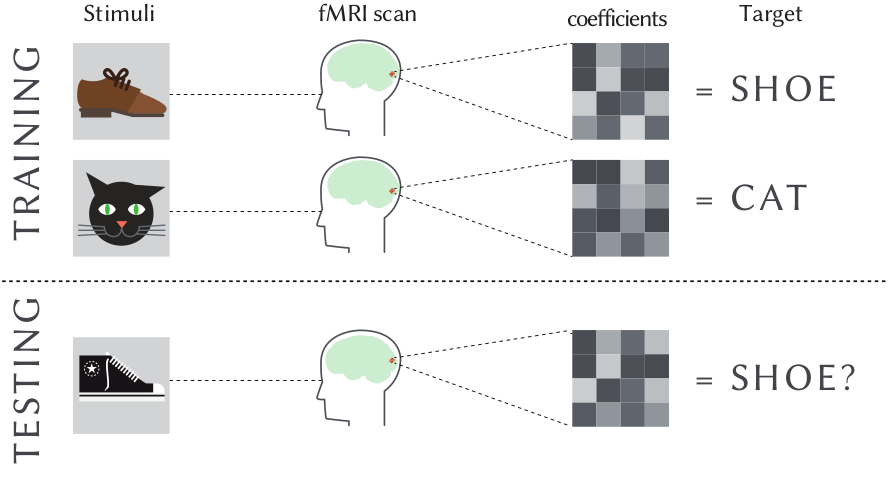
\includegraphics[width=1\linewidth]{figures/decoding.png}
  \caption{\textbf{Decoding} models mine
patterns of activity to discriminate
between cognitive states. Different
activation patterns reflect different mental states. For example,
those associated with different images viewed by the subject.
In a training phase, the classifier will
learn to discriminate between brain activity measured under different
cognitive states. In the testing phase the generalization performance of the trained model is
quantified by evaluating the classifier on the testing set and comparing
the output of the classifier with the true labels associated with
the stimuli. One can map the accuracy of the decoder to ...~\citep{dehaene1998}. Adapted from [Smith, 2013]}
\end{pagefigure}

\paragraph{Inference inference (or ``brain reading'').}
An alternative approach called \textit{inverse inference} (or ``brain-reading'')~\citep{dehaene1998,cox2003}, has been proposed in order to cope with the limitations of the afore-mentioned classical inference. Inverse inference relies on a pattern recognition, and aims at decoding the neural code by using machine-learning methods. Based on a set of brain activation maps, inverse inference builds a predictive model that can be used for predicting a behavioral target (age, sex, IQ, etc.) for a new set of images. The prediction accuracy of the model is used as a measure of the quantity of information about the cognitive task shared by the voxels. By construction, this approach is multivariate, and can provide more sensitive analysis than standard statistical parametric mapping procedure [Kamitani 05, Haynes 06]. Several methods have been tested for classification or regression of activation images (Linear Discriminant Analysis -- LDA, Support Vector Machines -- SVM, Lasso, Elastic net regression, and many others), but, in this problem, the major bottleneck remains the localization of predictive regions within the brain volume. Additionally, we have to deal with the curse of dimensionality, as the number of features (voxels, regions) is much larger ($\sim 10^5-10^6$ ) than the numbers of sample (images) ($\sim 10^2 - 10^3$ ), the latter being limited by the cost of acquisition. Thus the prediction method may overfit the training set and thus not generalize well to new samples.

\paragraph{Towards intepretable multi-variate models.}
To cope with the high dimensionality of the data, the learning method has to be
regularized. However, the spatial structure of the image is not
taken into account in standard regularization methods, so that the
extracted features are often hard to interpret.

\section{Sparsity and structure-inducing priors}
Sparsity and smoothness inducing priors can used to
perform jointly the prediction of a target variable and region
segmentation in multivariate analysis settings. Sparsity can be enforced by
penalizing the (sum of) absolute values of the regression coefficients, leading to the
so-called Lasso model. Smoothness can achieved in penalizing the spatial gradient of
the regression coefficients, to enforce smooth regions (``blobs'').
The Total-variation (TV)~\citep{rudin1992nonlinear} penalty has
proven to be particularly powerful for realizing such effects. Laplacian regularization
is an easier means to this end (because in leads to a differentiable problem),
but has weaker mini-max rates, and the visual effect is less appealing.

\begin{figure}[!htbp]
  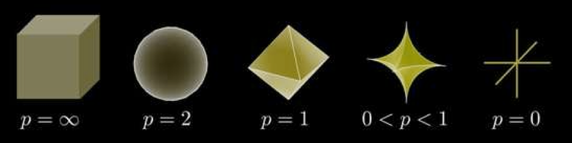
\includegraphics[width=1\linewidth]{figures/balls.png}
  \caption{$\ell_p$ unit ball for various values of $p$. The kinks
    in the cases $0 \le p \le 1$ impose sparsity. One notes however that, the
  cases $0 \le p < 1$ lead to non-convex intractable optimization problems.}
\end{figure}

\begin{marginfigure}[4cm]
  \centering
  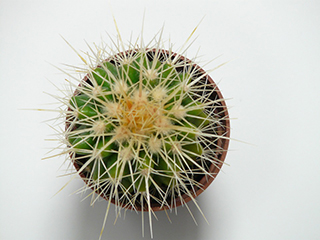
\includegraphics[width=1\linewidth]{figures/ball.jpg}
  \caption{$\ell_p$ ball with $0 < p \ll 1$.}
  \label{fig:flower}
\end{marginfigure}

In the context of neuro-imaging, sparsity and smoothness have been compiled to yield
regression coefficients which are faithful to known neurobiological organization of the brain,
while alleviating the risk of over-fitting due to inherently small-sample settings.
Specifically, it has been shown that one can employ priors like TV-$\ell_1$
~\citep{baldassarre2012,gramfort2013}, TV-ElasticNet~\citep{dubois2014predictive},
and GraphNet ~\citep{grosenick2013}
(aka Smooth-Lasso~\citep{hebiri2011})
%\footnote{Henceforth, we will use GraphNet and S-Lasso
%interchangeably.}
to regularize regression and classification
problems in brain imaging.

\paragraph{Notation.} We denote by ${\y} \in \mathbb{R}^{n}$ the targets to
be predicted (age, sex, IQ, etc.); the \textit{design matrix}
${\X}\in\mathbb{R}^{n \times p}$ are the masked (see Fig. \ref{fig:masking})
brain images related to the presentation of different
stimuli, or other brain acquisition (e.g gray-matter concentration
maps from anatomy, etc.). The integer $p$ is the number of voxels,
and $n$ the number of samples (images). In brain imaging, $n \ll p$;
typically, $p \sim 10^3-10^6$ (in full-brain analysis),
while $n \sim 10-10^3$ ($n$ being limited by the cost of acquisition,
etc.). $\nabla_x$ will denote the discrete spatial gradient operator
along the $x$-axis, $\nabla_y$ along the $y$-axis, etc.
Thus, at a voxel $j$, the spatial gradient of an image $\B{w}$ is a vector ${\nabla} {\w}(j) := [\nabla_{x} {\w}(j), \nabla_{y} {\w}(j), \nabla_{z} {\w}(j)]$, $\forall \w \in \mathbb R^p$.
This defines a linear operator $\nabla \in \mathbb R^{3p \times p}$ (the discrete 3D spatial gradient operator) from $\mathbb R^p$ to $\mathbb R^{3p}$. For a mixing constant $\rho \in [0, 1]$, $\nabla_\rho \in \mathbb R^{4p \times p}$ will denote the identity-augmented version of $\nabla$, defined by ${\nabla_\rho} {\w} := [(1-\rho)\nabla \w, \rho \w] \in \mathbb R^{4p}$.

%% Let $\mathcal P \subset \mathbb{R}^3$ be
%% the 3D image domain representing the region occupied by the brain --or
%% ROI (region of interest) thereof-- under  study, discretized regularly
%% on a finite grid.

  \begin{figure}[!htb] 
  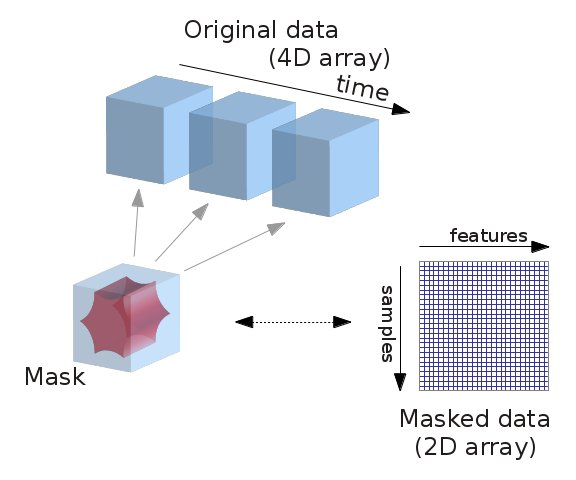
\includegraphics[width=1\linewidth]{figures/masking.jpg}
  \caption{\textbf{Masking} of volumic brain data (4D = 3D space + 1 \textbf{time} or \textbf{samples})
    to produce a design matrix required in standard machine learning (clustering, classification, regression, etc.). Each 3D volume considered is a sample point. The values of the voxels in this volume that lie in the mask are collected into a \textbf{feature vector}. All these vectors are vertically stacked to produce an $n$-by-$p$ design matrix $\X$, where $p$ is the number of voxels in the mask. The mask can be just the region of the 3D cube occupied by the brain, or a subset of such. In the latter case, this typically corresponds to Region-of-Interests (ROIs) deemed to be interesting for an experiment. The former case is referred to as ``full brain'', and the mask typically contains up to $p = $ millions of voxels. See ~\citep{abraham2014machine} for more details.}
  \label{fig:masking}
\end{figure}

\section{SpaceNet: sparse structured models for brain data}
Over time, a number of spatially regularized linear models have been proposed. These are mainly: Total-Variation (TV)~\citep{michel2011tv}, TV-$\ell_1$~\citep{baldassarre2012,gramfort2013}, GraphNet  ~\citep{grosenick2013,hebiri2011},
  TV-ElasticNet~\citep{dubois2014predictive}, Sparse Variation~\citep{eickenberg2015total}, and social-sparsity~\citep{kowalski2013social,varoquaux2016social}. These can all be synthesized into a general framework, referred to as \textit{SpaceNet}~\citep{spacenetohbm}, as follows
\begin{equation}
  \underset{\w \in \mathbb R^p}{\text{minimize }}E(\w) := \ell(\y,\X\w) + \alpha \mathcal P(\w).
    \label{eq:opt_pb}
\end{equation}
The coefficients ${\w}$ define a spatial map in over the brain (one value per voxel).
The term {$\ell(\y,\X\w)$} is the
  {loss / data-fit term}. Popular choices include:
  $$
  \ell(\y,\X\w) = \frac{1}{n}\sum_{i=1}^n\begin{cases}\frac{1}{2}(\B{X}^T_i\w - y_i)^2,
    &\mbox{ \text{ for least-squares regression}}\\
    \log(1+\exp(-y_i\X_i^T\w)),
    &\mbox{ \text{ for logistic regression}},\\
    (1 - y_i\X^T_i\w)_+,&\mbox{\text{ for hinge loss (used in SVMs)}}\\
      \vdots\end{cases}
    $$
$\mathcal P(\w)$ is the penalty term, which simultaneously imposes both sparsity and structure (blobs). The different spatial regularization
methods that have appeared in neuro-imaging literature can be cast into this
correspond to different choices of the convex penalty $\mathcal P$ acting on the extended gradient of the coefficients $\w$. Viz,

\begin{equation}
  \begin{split}
  \mathcal P(\w) = \begin{cases}
    \rho\|\w\|_1 + \frac{1}{2}(1-\rho)\|\nabla \w\|_{\text{Fro}}^2 = \sum_{j \in [\![p]\!]}\rho|w_j| + \frac{1}{2}(1-\rho)\|(\nabla \w)_j\|_2^2, &\mbox{ for GraphNet
      %~\citep{grosenick2013,hebiri2011}
    },\\
    \|\nabla_\rho \w\|_{1+2,1} = \rho\|\w\|_1 + \|\nabla \w\|_{2,1} = \sum_{j  \in [\![p]\!]}\rho|w_j| + (1-\rho)\|(\nabla \w)_j\|_2, &\mbox{ for isotropic TV-$\ell_1$
      %~\citep{baldassarre2012,gramfort2013}
    },\\
    \|\nabla_\rho \w\|_{1,1} = \rho\|\w\|_1 + (1-\rho)\|\nabla \w\|_{1,1} = \sum_{j  \in [\![p]\!]}\rho|w_j| + (1-\rho)\|(\nabla \w)_j\|_1, &\mbox{ for anisotropic TV-$\ell_1$
    },\\
    \|\nabla_\rho \w\|_{2,1} = \sum_{j  \in [\![p]\!]}\|(\nabla_\rho \w)_j\|_2, &\mbox{ for Sparse Variation
      %~\citep{eickenberg2015total}
    },\\
      \vdots
    \end{cases}
  \end{split}
  \label{eq:penalty}
\end{equation}
where
\begin{itemize}
  \item $\alpha > 0$ is a regularization parameter controls the total amount of regularization;
\item $\rho$ ($0 < \rho \le 1$) is a mixing constant between
  the {sparsity-inducing} $\ell_1$ part and the
  {cluster-promoting} part of the penalty term.
  The particular case {$\rho = 1$} corresponds to the usual Lasso. Vanilla TV  ~\citep{michel2011tv} corresponds to TV-$\ell_1$ with $\rho = 0$.
\item The matrix $\nabla_\rho$ is the extended discrete gradient operator defined in the table of notations.
\end{itemize}
\begin{shaded}
\paragraph{Bayesian interpretation.} The penalties $\mathcal P(\w)$ in \eqref{eq:opt_pb} admit a Bayesian interpretation as a prior on the distribution of the coefficients $\w$
\begin{equation}
  \label{eq:bayesian}
  p_{\alpha,\rho}(\w) \propto \exp(-\mathcal P(\w)).
\end{equation}
For example, the GraphNet~\citep{grosenick2013,hebiri2011}, the penalties $\mathcal P(\w)$ penalty corresponds to
\begin{equation}
p_{\alpha,\rho}(\w) \propto    \prod_{j=1}^p\exp(-\alpha\rho |w_j|)\prod_{j=1}^p\exp\left(-\alpha(1-\rho)\sum_{l \sim \text{neigh}(j)}w_j\Delta_{j,l}w_l\right).
\end{equation}
\end{shaded}

\begin{marginfigure}
  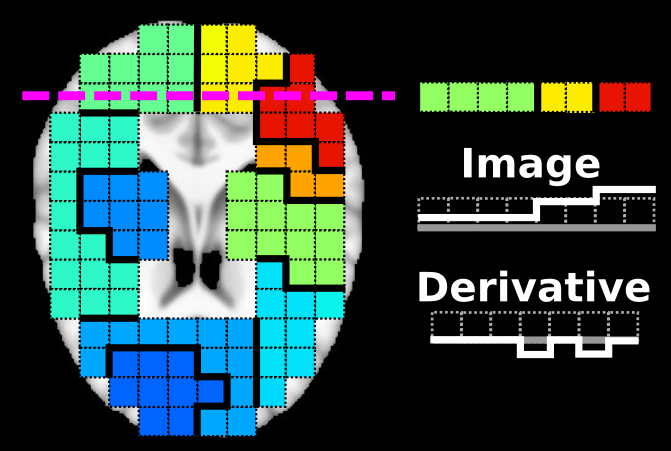
\includegraphics[width=1\linewidth]{figures/tv_cartoon_horizontal.png}
  \caption{A cartoon showing a sparse and blobby (step-wise constant / cartoon-like) brain map,
  as would be sought for by Total-Variation regularization \eqref{eq:ss}...}
  \label{fig:roi}
\end{marginfigure}

SpaceNet models \eqref{eq:main_pb} result brain maps which are both
sparse (i.e regression coefficients $\w$ are zero everywhere, except at
predictive voxels) and structured (blobby). See Fig. \ref{fig:roi}. The superiority of such
methods over methods without structured priors like the Lasso, ANOVA,
Ridge, SVM, etc. for yielding more intepretable maps and improved
prediction scores is now well established. See for example
 ~\citep{baldassarre2012,gramfort2013}. These priors are fast becoming
popular for brain decoding and segmentation. Indeed, they leverage a
feature-selection function
(since they limit the number of active voxels),
and also a structuring function
(since they penalize local
differences in the values of the brain map). For example, see Fig.
\ref{fig:spacenet_maps}.
Also, such priors produce state-of-the-art methods for automatic
extraction of functional brain atlases  ~\citep{abraham2013}.

\begin{shaded}
  \paragraph{Submodular interpretation of TV.} We note that anisotropic TV penalty \eqref{eq:penalty} on
  an arbitrary (undirected) graph $G = (V,E)$ is the \textit{Lovasz extension} of the \textit{cut-function}
  $F : 2^V \rightarrow \mathbb N$, $S \mapsto "\text{number of edges between } S \text{ and }V\setminus S"$,
defined by $F^L(x) := \mathbb E_{\lambda \sim \mathcal U([0,1])}[F(\{v \in V|x_v \ge \lambda\})]$, for all $x \in [0,1]^{\#V}$.
\end{shaded}

\begin{figure}[!htbp]
  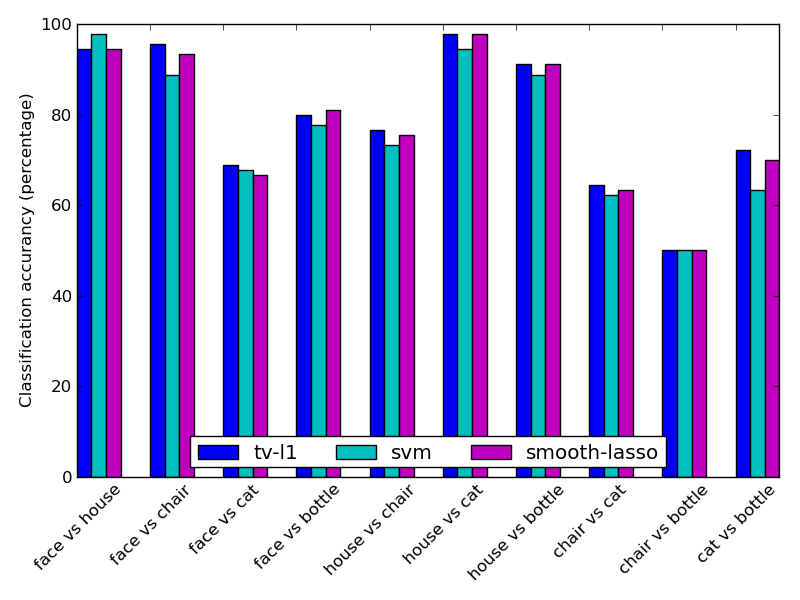
\includegraphics[width=1\linewidth]{figures/haxby_barchart.png}
  \caption{Bar chart showing percentage classification on leftout, for one-vrs-one classification on the visual recognition dataset~\citep{haxby2001}.
  }
  \label{fig:spacenet_bars}
\end{figure}

\section{Methods}
The SpaceNet model leads to difficult non-smooth mathematical optimization problems making their implementation and practical usability challenging.~\citep{dohmatob2014benchmarking} benchmarked a rich variety of cutting-edge solvers for such problems, and gave crucial recommendations on how to effectively implement these algorithms in practice. In these benchmarks, the FISTA algorithm emerged as the go-to algorithm for the TV-L1 problem~\citep{dohmatob2015speeding}. These hints have been carefully used in implementing SpaceNet. Also as a preprocessing step, we use univariate feature-screening (ANOVA) to eliminate voxels which are irrelevant to the learning problem, thus reducing the size of the problem. As a result the implementation of SpaceNet is fast, robust, and automatically sets its parameters (internal cross-validation). All these technical details will be properly presented in the next few chapters.

\subsection{Cross-validation}
Cross-validation (e.g see ~\citep{stone74}) is a technique used to protect against overfitting in a predictive model, particularly in a case where the amount of data may be limited. In cross-validation, you make a fixed number of folds (or partitions) of the data, run the analysis on each fold, and then average the overall error estimate. This gives an (asymptotically) unbiased estimate of the true generalization error of the model. 
Two major types of cross-validation are K-Fold and Leave-One-Out (LOO).

\paragraph{K-Fold cross-validation.}
One iteration of the K-fold cross-validation is performed in the following way: First, a random permutation of the sample set is generated and partitioned into K subsets ("folds") of about equal size. Of the K subsets, a single subset is retained as the validation data for testing the model (this subset is called the "testset"), and the remaining K - 1 subsets together are used as training data ("trainset"). Then a model is trained on the trainset and its accuracy is evaluated on the testset. Model training and evaluation is repeated K times, with each of the K subsets used exactly once as the testset.
The case of a 5-fold cross-validation with 30 samples is illustrated in Fig. \ref{fig:cv}.

\paragraph{Leave-One-Out cross-validation.}
As the name suggests, leave-one-out cross-validation involves using a single sample from the original sample set as the validation data, and the remaining samples as the training data. This is repeated such that each sample in the sample set is used exactly once as the validation data. This is the same as K-fold cross-validation where K is equal to the number of samples in the sample set.
In LOO, there is no need in generating random permutations and in repeating it, because the training and validation datasets for each of the folds are always the same, and therefore the result of the accuracy estimation is determined.

\begin{figure}
  \subfloat[1 iteration of 5-Fold cross-validation]{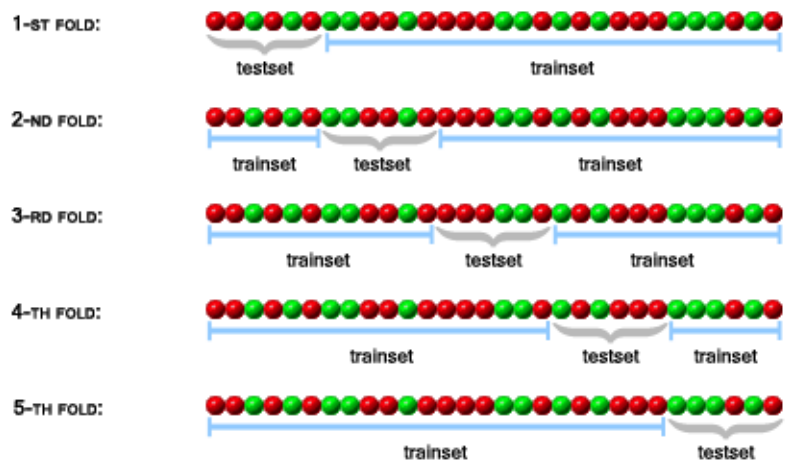
\includegraphics[width=1\linewidth]{figures/cv_folds.png}}\\
  \subfloat[Parameter grid]{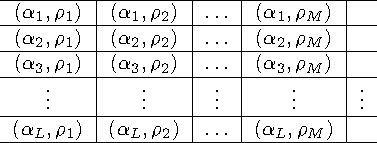
\includegraphics[width=1\linewidth]{figures/cv_grid.pdf}}
  \caption{\textbf{Model-selection} via cross-validation.
\textbf{\textit{(a)}} K-Fold cross-validation, illustrated
here for the case $K = 5$, involves
taking the available data and partitioning it into $K$ groups. Then
$K - 1$ groups are used to train a set of models that are then
evaluated on the remaining group. Adapted from \url{http://genome.tugraz.at/proclassify/help/pages/XV.html}.
\textbf{\textit{(b)}} $L \times M$ grid over which to search for optimal configuration in
a model with two hyper-parameters $\alpha$ and $\rho$. For a model like SpaceNet \eqref{eq:main_pb}, the grid is is constrained to verify $0 \le\alpha_L < \ldots < \alpha_1 = \alpha_{\text{max}}$ and $0 \le \rho_M < \ldots < \rho_1 \le 1$, with $L = 10$ and $M = 3$ typically, given a total of $LM = 30$ models to compare. In chapter \ref{chap:speeding}, we show how \textit{early-stopping} and other heuristics can be used to make the total cost much more effective than just fitting $LM$ models in a CV loop. }
  \label{fig:cv}
\end{figure}

\paragraph{Model-selection via cross-validation.}
One can instrument cross-validation to tune the hyper-parameters of a model like SpaceNet \eqref{eq:main_pb}, by selected the configuration of model parameters with least cross-validation error. The number of models fitted is proportional to the size of the parameter grid --i.e exponential in the number of parameters to tune-- and therefor can become prohibitive in case there are many free hyper-parameters in the model. Also, since some of the data has to be set aside for validation, cross-validation in very small sample settings (e.g e few tenths, as is the in some neuroimaging experiments) may be troublesome as the error estimates then have very high variance. A reasonable alternative in such situations are SURE (short for \textit{Stein's Unbiased Risk Estimator}~\citep{stein1981})-based methods,
which are applicable whenever a procedure for obtaining (an unbiased estimate of) the number of degrees of freedom of the model is available. This is the case with the models like the ElasticNet and
GraphNet~\citep{hebiri2011}. Recently, ~\citep{sugar} has proposed a STEIN-based technique for structured models with many hyper-parameters.


\subsection{How SpaceNet compares against classical unstructured models}
\paragraph{Classification.}
We compared SpaceNet (TV-L1 and GraphNet / Smooth-Lasso priors) with an SVM (Support Vector Machine) on the visual-recognition dataset~\citep{haxby2001}. This dataset consists of 6 subjects with 12 runs per subject. In each run, the subjects passively viewed images of eight object categories, grouped in 24-second blocks separated by intermittent rest periods. This experiment is a classification task: predicting the object category. The design matrix is made of time-series from the full-brain mask of $p=23,707$ voxels over 216 TRs (Repetition Times), of a single subject (subj1). 126 TRs were used for training all the models, whilst testing was done on 90 left-out TRs. The results are depicted in Figures 1 (bar chat) and 2 (brain maps).

\begin{pagefigure}%[!htb] 
  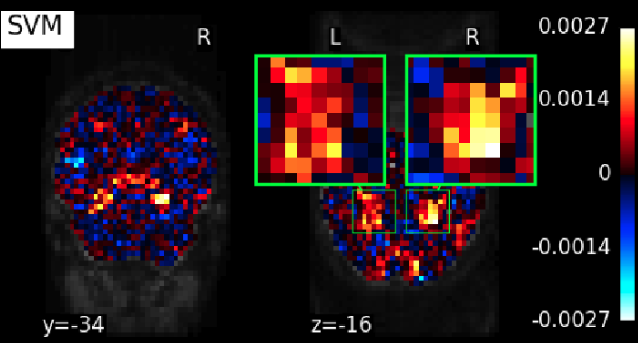
\includegraphics[width=.32\linewidth]{figures/svm.png}
  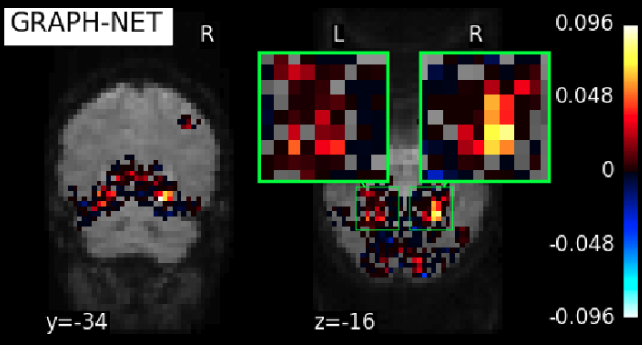
\includegraphics[width=.32\linewidth]{figures/graphnet.png}
  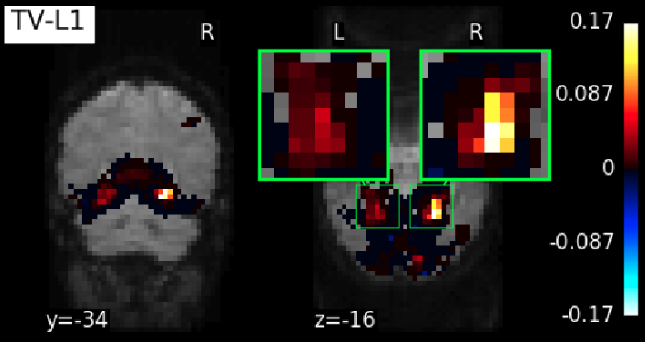
\includegraphics[width=.32\linewidth]{figures/tvl1.png}  
  \caption{The figure shows results of comparing the SpaceNet  models TV-$\ell_1$ and
    Graph-Net against an SVM (Support Vector Machine) classifier on
    the visual-recognition dataset  ~\citep{haxby2001}
    As can be seen from the figure, SpaceNet priors (TV-$\ell_1$, GraphNet, etc.)
    yield stable and more intepretable maps by enforcing smoothness on the coefficients while segmenting predictive regions (blobs) from noisy background.}
  \label{fig:spacenet_maps}
\end{pagefigure}

\paragraph{Regression.}
In ~\citep{gramfort2013}, the authors compared several models on a dataset in which subjects were presented with mixed (gain/loss) gambles, and decided whether they would accept each gamble~\citep{jimura2012}. No outcomes of these gambles were presented during scanning, but after the scan three gambles were selected at random and played for real money. The prediction task here is to predict the magnitude of the gain and thus a regression on a continuous variable. The full dataset of 16
subjects with 48 3D scans each, making up for a total of $n=768$ samples with approximately $p=3.3 \times 10^4$ voxels. The prediction here is inter-subject: the estimator
learns on some subjects and predicts on left out subjects.
The results are shown in Fig. \ref{fig:tvl1_regression}.

\begin{figure}[!htbp] 
  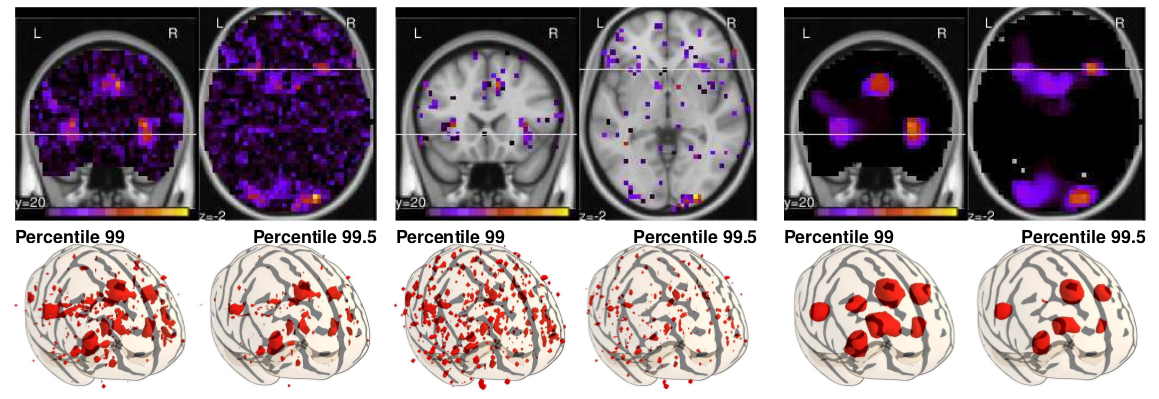
\includegraphics[width=1\linewidth]{figures/gramfort_tvl1.png}
  \caption{Results on fMRI data from [4] (from left to right F-test, ElasticNet and TV-L1). The TV-L1 regularized model segments neuroscientifically
    meaningful predictive regions in agreement with univariate statistics while the ElasticNet yields sparse although very scattered non-zero weights. Source: adapted from ~\citep{gramfort2013}.}
  \label{fig:tvl1_regression}
\end{figure}

\section{Conclusion}
We have presented SpaceNet, a family of priors for brain decoding that enforce both sparsity and structure, leading to better prediction scores and intepretable brain maps. We believe that such priors will become commonplace in future.
In the next few chapters, we open the ``black-box'' and develop from ground-up, the details of such models, including their practical implementation on a computer.

% \clearpage
\bibliographystyle{plainnat}
\bibliography{bib_all}
 % SpaceNet model
\begin{fullwidth}
\chapter{Structured priors for analyzing brain data: the models and algorithms}\label{chap:hrf_estimation}
\end{fullwidth}

\markright{{~{\rm \ref{chap:hrf_estimation}}. Data-driven HRF estimation}\hfill}{}

% \newthought{We have seen} in Chapter~\ref{chap:stats_fmri} that%  encoding and decoding models take 
% as input  brain activation coefficients (also known as activation patterns or beta-maps). These are usually computed by means of the general linear model (GLM), which
% relies on a \mbox{data-independent} \emph{canonical} form of the hemodynamic response function
% (HRF).


% In this chapter we describe a novel method for the simultaneous estimation of HRF and activation coefficients based on low-rank modeling, forcing the estimated HRF to be equal across events or experimental conditions,
%  yet permitting it to differ across voxels. The estimation of this model leads to
% an optimization problem that we propose to solve with using a
% \mbox{quasi-Newton} method, exploiting fast gradient computations. 
% We compare 10 different HRF modeling methods in terms of encoding and decoding
% score on two different datasets. These results show that the \mbox{R1-GLM} model
% outperforms competing methods in both encoding and decoding
% settings, positioning it as an attractive method both from the points of view
% of accuracy and computational efficiency.

% \hspace{20pt}
% \begin{shaded}
% The contributions developed in this chapter have been published in:
% \begin{itemize}
% \item F. Pedregosa, M. Eickenberg, P. Ciuciu, and B. Thirion, \emph{``Data-driven HRF estimation for encoding and decoding models''} NeuroImage, Volume 104, 1 January 2015, Pages 209-220.

% \item F. Pedregosa, M. Eickenberg, B. Thirion, and A. Gramfort, \emph{“HRF estimation improves sensitivity of fMRI encoding and decoding models”} Proc. 3nd Int. Work. Pattern Recognit. NeuroImaging, 2013.
% \end{itemize}
% \end{shaded}

% \newpage
% \vspace*{\fill}
% \minitoc
% \vspace*{\fill}
% \newpage


\section{Sparsity and smoothness priors for improved estimation in high dimensions}
\newthought{Michel et al. 2011, Baldasarre et al. 2012, Gramfort et al. 2013, Abraham et al. 2013, Dohmatob et al. 2014(5), Varoquaux et al. 2016}, ...

\section{Efficient optimization of sparsity and smoothness regularized models}
\newthought{In our PRNI 2014 (``Benchmarking ...'') and 2015 (``Speeding-up ...'') papers}, ...

% \begin{marginfigure}[4cm]
% \hspace{-20pt}\includegraphics[width=1.2\linewidth]{chapter_3/hrfs_age.pdf}
% \caption{
% 	The HRF can vary substantially between subjects, brain regions and age. In \citet{colonnese2007development}, the authors studied the evolution of the HRF across age in rats. By comparing fMRI measurements with electrophysiological recordings, they observed two significant trends as age increased: growing amplitude and decreasing time to peak. In the figure, estimated HRF for three groups of rats (with age P13-15 < P20-30< Adult). Source: \citep{colonnese2007development}. A comparison of the HRF in human subjects was performed in~\citep{badillo2014multi}.
% }
% \end{marginfigure}


% fMRI acquisitions consist of successive brain scans, given in intervals ranging from 1 to 4 seconds. The extraction of time-independent \gls{activation coefficient} from the BOLD time course is commonly done with a model known as Linear General Model
% (GLM)~\citep{Friston1995}. While
% this approach has been successfully used in a wide range of studies, it does
% suffer from limitations~\citep{Poline2012}. For instance, the GLM commonly
% relies on a \mbox{data-independent} \emph{reference} form of the hemodynamic response function
% (HRF) to estimate the activation coefficient (also known as \emph{canonical HRF}). However it is
% known~\citep{Handwerker2004,Badillo2013} that the shape of this response function
% can vary substantially across subjects, age and brain regions. This suggests that an adaptive modeling of this
%  response function should improve the accuracy of subsequent analysis.

% % \emph{feature-extraction} model that extracts 

% % In this section we describe a method that allows to estimate time-independent \gls{activation coefficient} given the BOLD time course. {\blue Feature extraction}. This model is known as the \emph{general linear model}~\citep{Friston1995}. In this chapter we describe the main assumptions behind this model: a known form of the hemodynamic response function and the linear-time-invariant property between the BOLD signal and the neural response. 

% % We have seen in Chapter 2 that both encoding and decoding models take as input voxel-wise activation coefficients. These are commonly are computed by means of the General Linear Model
% % (GLM)~\citep{Friston1995}. While
% % this approach has been successfully used in a wide range of studies, it does
% % suffer from limitations~\citep{Poline2012}. For instance, the GLM commonly
% % relies on a \mbox{data-independent} \emph{reference} form of the hemodynamic response function
% % (HRF) to estimate the activation coefficient (also known as \emph{canonical HRF}). However it is
% % known~\citep{Handwerker2004,Badillo2013} that the shape of this response function
% % can vary substantially across subjects, age and brain regions. This suggests that an adaptive modeling of this
% %  response function should improve the accuracy of subsequent analysis.

% To overcome the aforementioned limitation, Finite Impulse Response (FIR) models have been
% proposed within the GLM framework~\citep{Dale1999,Glover1999}.
% These models do not assume any particular shape for the HRF and amount to
% estimating a large number of parameters in order to identify it. 
% While the FIR-based modeling makes it possible to estimate the
% activation coefficient and the HRF simultaneously, the increased flexibility
% has a cost. The estimator is less robust and prone to overfitting, i.e. to generalize poorly to unseen data. 
% In general, FIR
% models are most appropriate for studies focused on the characterization of the
% shape of the hemodynamic response, and not for studies that are primarily
% focused on detecting activation~\cite[Chapter~5]{Poldrack}.

% Several strategies aiming at reducing the number of degrees of freedom of the
% FIR model - and thus at limiting the risk of overfitting - have been proposed.
% One possibility is to constrain the shape of the HRF to be a linear
% combination of a small number of basis functions. A common choice of basis is 
% formed by three elements consisting of a reference HRF as well as its time and dispersion
% derivatives~\citep{friston1998nonlinear}, although it is also possible to compute a
% basis set that spans a desired function
% space~\citep{Woolrich2004}. More generally, one can also define a parametric
% model of the HRF and estimate the parameters that best fit this
% function~\citep{Lindquist2007}. However, in this case the estimated HRF may no longer be a linear function of the input parameters. 

% Sensitivity to noise and overfitting can also be reduced through
% regularization. For example, temporal regularization has been used in the
% smooth FIR ~\citep{Goutte2000,Ciuciu2003,Casanova2008} to favor solutions with
% small second order time derivative. These approaches require the setting of
% one or several hyperparameters, at the voxel or potentially at the parcel
% level (if several voxels in a pre-defined parcel are assumed to share some aspects of the HRF time course). Even if efficient techniques such as generalized   
% \mbox{cross-validation}~\citep{golub1979generalized} can be used to choose the
% regularization parameters, these methods are inherently more costly than 
% \mbox{basis-constrained} methods. \mbox{Basis-constrained} methods also require
% setting the number of basis elements; however, this parameter is not
% continuous (as in the case of regularized methods), and in practice only few
% values are explored: for example the 3-element basis set formed by a reference HRF
% plus derivatives and the FIR model.  This paper focuses on basis-constrained
% regularization of the HRF to avoid dealing with hyperparameter selection with
% the goal of remaining computationally attractive.  A different approach to
% increase robustness of the estimates consists in linking the estimated HRFs
% across a predefined brain parcel, taking advantage of the spatially dependent nature of
% fMRI~\citep{Wang2013}. However, \mbox{hemodynamically-informed}
% parcellations~\citep{Chaari2012,Badillo2013a} rely on the computation of 
% a large number of estimations at the voxel or \mbox{sub-parcel} level.
% In this setting, the development of voxel-wise estimation procedures is complementary to the
% development of parcellation methods in that more robust estimation
% methods at the voxel level would naturally translate into more 
% robust parcellation methods. In this thesis we focus on voxel-wise
% estimation methods.


% \paragraph{Contribution}

% In this chapter we have described a method for the simultaneous estimation of HRF and activation coefficients based on low-rank modeling. While the assumptions of this model are not novel (cf.~\citep{Makni2008,vincent2010spatially,Degras2014}), the formulation of this model as a least squares problem with a rank-one constraint is a novel contribution. This formulation allows to efficiently solve the problem using gradient-based methods.
% Finally, we evaluate the proposed model on three publicly available datasets. 

% % {\blue With respect to the work published in ~\citep{Pedregosa2015209}, we have included in this chapter the results on a new datasets and examined the gain obtained by this model across different regions of the brain}.

\section{A small result on the rate of convergence of the ADMM algorithm}
\newthought{In our ICASSP 2016 paper}, ...

% In this section we describe different methods for extracting the HRF and
% activation coefficients from BOLD signals. We will refer to each different
% stimulus as {\it condition} and we will call {\it trial} a unique presentation
% of a given stimulus. We will denote by $k$ the total number of stimuli, $\B{y} \in \RR^n$
% the BOLD signal at a single voxel and $n$ the total number of images acquired.

\section{Generalized online dictionary learning: richer penalties on the components}
\newthought{In our NIPS 2017 paper}, ...




% The reference HRF models a general response function that has been proven successful under a wide range of circumstances. However, a number of studies have shown that the shape of the hemodynamic response differ substantially among subjects~\citep{Aguirre1998360} and brain regions~\citep{Schacter1997259}. One popular approach to model small offsets in the time to peak and dispersion is to consider that the HRF is modeled from a basis set consisting of the reference HRF plus its derivative with respect to time and dispersion (see Figure~\ref{fig:hrf_basis}). The rationale for considering this basis set comes from the fact that it corresponds to the first-order approximation to the Taylor expansion of the reference HRF. Given the reference HRF, $h(t)$, a time-shifted version of the hemodynamic response can be described as $h(t + \delta)$. A Taylor series expansion of $h(t + \delta)$ with respect to $\delta$ gives the approximation $h(t) + \delta h'(t) + \ldots$~, implying that small offsets can be modeled by considering a linear combination of the reference HRF plus its time derivative. In similar fashion we can model small perturbations in dispersion (the width of the response) by considering the reference HRF plus its dispersion derivative. 


% \begin{figure*}
% \includegraphics[width=.5\linewidth]{figures/chapter_1/canonical_hrf_basis.pdf}
% \includegraphics[width=.5\linewidth]{figures/chapter_1/canonical_hrf_generated.pdf}
% \caption{A popular basis set to generate a family of HRF functions is the ``reference HRF plus derivatives''. In the left plot, we show a reference HRF together with its time and dispersion derivatives. This basis set can model small variations in temporal shifts and dispersion with respect to the reference HRF. In the right plot we show a sample set of HRFs generated by this basis. The weights of these response functions are Gaussian random vectors centered around the reference HRF.}\label{fig:hrf_basis} 
% \end{figure*}

% A popular example of basis set is presented in Figure~\ref{fig:hrf_basis} and consists of the reference HRF plus its time and dispersion (width) derivatives. While in the GLM with fixed HRF each regressor of the design matrix consisted of the convolution of the reference HRF with the stimulus function, in this case each regressor consist in the convolution of a basis element with the stimulus function. This results in a  design matrix of size $n \times d k$ instead of $n \times k$, where $d$ is the number of basis elements. If $d=1$ and the basis element is the reference HRF, then this setting coincides with the standard GLM. A least squares estimate of the activation coefficients $\hat{\bfbeta} = \argmin_{\bfbeta}\|\B{y} - \B{X}\bfbeta \|^2$ will result in a vector of $d$ elements for each condition. 


% The design matrix of a GLM using the basis set of the ``refence HRF plus derivatives'' is shown in Figure~\ref{fig:glm1}. The columns in this design matrix are each one of the basis elements convolved with the stimulus function for the different conditions.




% \section{Basis and rank-constrained GLM}

% In the basis-constrained GLM, the HRF estimation is performed 
% independently for each condition. This method works reliably whenever
% the number of conditions is small, but in experimental designs with a large
% number of conditions it performs poorly due to the increased variance of the estimates.
% % put ref?

% % In this model we promote a common HRF
% % across the various stimuli, which should result in more robust estimates~\citep{Makni2008,vincent2010spatially}.
% In this work we consider a model in which a common HRF is shared
% across the different stimuli. Besides the estimation of the HRF,
% a unique coefficient is obtained per column of our event
% matrix. This amounts to the estimation of $k + d$ free parameters
% instead of $k \times d$ as in the standard basis-constrained GLM setting.

% The novelty of our method stems from the observation that the formulation of the GLM with a
% common HRF across conditions translates to a rank constraint on the vector of estimates. 
% This assumption amounts to enforcing the vector of
% estimates to be of the form $\bfbeta_{\B{B}} = [\mathbf{h} {\beta}_1, \mathbf{h} \beta_2, \cdots, \mathbf{h}
% \beta_k]$ for some HRF $\mathbf{h} \in \RR^d$ and a vector of coefficients $\bfbeta \in \RR^k$. More compactly, this can be written as $\bfbeta_{\B{B}} = \vecop(\B{h}
% \bfbeta^T)$. This can be
% seen as a constraint on the vector of coefficients to be the vectorization of a rank-one
% matrix, hence the name {\it Rank-1 GLM (R1-GLM)}.


% \begin{figure*}[t]
% \centering \includegraphics[width=0.8\linewidth]{figures/chapter_1/glm_3hrf.pdf}
% \caption{A basis-constrained GLM design matrix. The basis set consists of the reference HRF plus its time and dispersion derivative. As in the GLM introduced in Chapter~\ref{chap:intro_fmri} (Fig.~\ref{fig:glm1}), each column is the convolution of one basis function with the stimulus function. Here, the usage of 3 basis functions (instead of one) results in a design matrix with $3 k$ regressors}\label{fig:glm_3hrf}
% \end{figure*}


% In this model, the coefficients have no longer a closed form expression,
% but can be estimated by minimizing the following loss function. Given $\B{X}_{\B{B}}$ and $\B{y}$ as before, $\B{Z} \in \RR^{n \times q}$ a matrix of nuisance parameters such as drift regressors, we define $F_{\text{R1}}(\B{h}, \bfbeta, \bfomega, \B{X}_{\B{B}}, \B{y}, \B{Z}) = \frac{1}{2}\|\mathbf{y} - \mathbf{X}_{\B{B}} \vecop(\B{h} \bfbeta^T) - \B{Z} {\bfomega}\| ^2$ to be the objective function to be minimized. The optimization problem reads:
% %
% \begin{eqnarray}
% \label{eq:r1}
% \begin{aligned}
% \hat{\B{h}}, ~\hat{\bfbeta},~ \hat{\bfomega} ~=~& \argmin_{\B{h}, \bfbeta, {\bfomega}} ~ F_{\text{R1}}(\B{h}, \bfbeta, \bfomega, \B{X}_{\B{B}}, \B{y}, \B{Z})\\
% &\text{subject to } \|\B{B} \B{h}\|_{\infty} = 1 \text{ and } \langle \B{B} \B{h}, \B{h}_{\text{ref}}\rangle > 0 \enspace ,
% \end{aligned}
% \end{eqnarray}
% %
% The norm constraint is added to avoid the scale ambiguity between $\B{h}$ and $\bfbeta$
% and the sign is chosen so that the estimated HRF correlates
% positively with a given reference HRF $\B{h}_{\text{ref}}$.
% Otherwise the signs of the HRF and $\bfbeta$ can be simultaneously flipped without changing
% the value of the cost function. Within its feasible set, the optimization problem
% is {\it smooth} and is convex with respect to $\B{h}$, $\bfbeta$ and $\bfomega$,
%  however it is not {\it jointly convex} in variables $\B{h}$, $\bfbeta$ and $\bfomega$.

% From a practical point of view this formulation has a number of advantages.
% First, in contrast with the GLM without rank-1 constraint the estimated
% coefficients are already factored into the estimated HRF and the activation
% coefficients. That is, once the estimation of the model parameters
% from Eq.~\eqref{eq:r1} is obtained, $\hat{\bfbeta}$ is a vector of size $k$ and $\hat{\B{h}}$ is a
% vector of size $d$ that can be both used in subsequent analysis, while in models
% without rank-1 constraint only the vector of coefficients (equivalent to 
% $\text{vec}(\B{h} \bfbeta^T)$ in rank-1 constrained models) of size $k
% \times d$ is estimated. In the latter case, the estimated HRF and the beta-maps
% still have to be extracted from this vector by methods such as normalization by the peak of the HRF,
% averaging or projecting to the set of Rank-1 matrices.

% Second, it is readily adapted to prediction on unseen trials. While for
% classical (non rank-1 models) the HRF estimation is performed per condition with no HRF associated with unseen conditions, in this setting, because the
% estimated HRF is linked and equal across conditions it is natural to use this
% estimate on unseen conditions. This setting occurs often in encoding models 
% where prediction on unseen trials is part of the cross-validation procedure.

% This model can also be extended to a parametric HRF model. That is,
% given the hemodynamic response defined as a function $h: \RR^{d_1} \to \RR^d$ of some parameters
% $\bfalpha$, we can formulate the analogous model of Eq.~\eqref{eq:r1} as an
% optimization over the parameters $\bfalpha$ and $\bfbeta$ with the design matrix
% $\B{X}_{\text{FIR}}$ given by the convolution of the event matrix with the FIR basis:
% %
% \begin{eqnarray}
% \label{eq:r1_parametric}
% \begin{aligned}
% \hat{\bfalpha}, ~\hat{\bfbeta}, ~\hat{\bfomega} ~=~&\argmin_{\bfalpha, \bfbeta, \bfomega} 
% F_{\text{R1}}(h(\bfalpha), \bfbeta, \bfomega, \B{X}_{\text{FIR}}, \B{y}, \B{Z}) \\
% &\text{subject to } \| h(\bfalpha)\|_{\infty} = 1  \text{ and } \langle h(\bfalpha), \B{h}_{\text{ref}} \rangle > 0
% \end{aligned}
% \end{eqnarray}

% In section \ref{sub:optim} we will discuss optimization strategies for both
% models.

% % \section{Alternative formulations}

% % We present two alternative formulations

% \section{Extension to separate designs}

% \begin{marginfigure}[8cm]
% \center \includegraphics[width=.6\linewidth]{chapter_3/ls-s.pdf}
% \caption{In the GLM with separate designs model of~\citet{Mumford2012}, the design matrix contains two regressors. The first one is the
% regressor associated with a given condition and the second one is the sum of all
% other regressors. Source: \citep{Turner2012}}
% \end{marginfigure}

% An extension to the classical GLM that improves the estimation with correlated
% designs was proposed in~\citep{Mumford2012}.
% In this setting, each voxel is modeled as a linear combination of two
% regressors in a design matrix $\B{X}_\text{GLM}$. The first one is the
% regressor associated with a given condition and the second one is the sum of all
% other regressors. This results in $k$ design matrices, one for each condition.
% The estimate for a given condition is given by the first element in the two-dimensional
% array ${\B{X}_{\text{S}i}}^{\dagger} \B{y}$, 
% where $\B{X}_{\text{S}i}$ is the design matrix for
% condition $i$. We will 
% denote this model GLM with separate designs (GLMS). It has been reported to find
% a better estimate in rapid event designs leading to a boost in accuracy for
% decoding tasks~\citep{Mumford2012, Schoenmakers2013, Lei2013}.

% This approach was further extended in~\citep{Turner2012} to
% include FIR basis instead of the predefined canonical function. Here we employ it 
% in the more general setting of a  
% predefined basis set. Given a set of basis
% functions we construct the design matrix for condition $i$ as the columnwise
% concatenation of two matrices $\B{X}^0_{\text{BS}i}$ and $\B{X}^1_{\text{BS}i}$.
% $\B{X}^0_{\text{BS}i}$ is given by the columns associated
% with the current condition in the GLM matrix and $\B{X}^1_{\text{BS}i}$ is
% the sum of all other columns.
% In this case, the vector of estimates is given by the first $d$ vectors of
% $\B{X}_{\text{BS}i}^{\dagger} \B{y}$. See~\citep{Turner2012} for a more complete description of the matrices $\B{X}^0_{\text{BS}i}$ and $\B{X}^1_{\text{BS}i}$.

% It is possible to use the same rank-1
% constraint as before in the setting of separate designs, linking the HRF 
% across conditions. We will refer to this model as \emph{Rank-1 GLM with separate designs (R1-GLMS)}. In this case the objective function has the form
% $F_{\text{R1-S}}(\B{h}, \bfbeta, \bfomega, \B{r}, \B{X}_{\B{B}}, \B{y}, \B{Z}) = \frac{1}{2}\sum_i^k \|\B{y} - \beta_i \B{X}^0_{\text{BS}i} \B{h} - r_i \B{X}^1_{\text{BS}i} \B{h} - \B{Z} \bfomega\| ^2 $, where $\B{r} \in \RR^d$ is a vector representing the activation of all events except the event of interest and 
% will not be used in subsequent analyses. We can 
% compute the vector of estimates $\hat{{\bfbeta}}$ as the solution to the optimization
% problem
% %
% \begin{eqnarray}
% \label{eq:r1_separate}
% \begin{aligned}
% \hat{\bfbeta}, ~\hat{\bfomega},~\hat{\B{h}},~\hat{\bf{r}} ~= ~&\argmin_{\B{h}, \bfbeta, \bfomega, \B{r}} F_{\text{R1-S}}(\B{h}, \bfbeta, \bfomega, \B{r}, \B{X}_{\B{B}}, \B{y}, \B{Z}) \\
% &\text{subject to } \|\B{B} \B{h}\|_{\infty} = 1 \text{ and } \langle \B{B} \B{h}, \B{h}_{\text{ref}} \rangle > 0
% \end{aligned}
% \end{eqnarray}
% %


% \section{Optimization}
% \label{sub:optim}


% For the estimation of rank-1 models on a full brain volume, a  model is estimated at each voxel separately. Since a typical brain volume contains more than 40,000 voxels, the efficiency of the estimation at a single voxel is of great importance. In this section we will detail an efficient procedure based on quasi-Newton methods for the estimation of R1-GLM and R1-GLMS models on a given voxel.


% One approach to minimize \eqref{eq:r1} is to alternate the minimization
% with respect to the variables $\bfbeta$, $\B{h}$ and $\bfomega$. By recalling the Kronecker product identities~\cite[Chapter 4.3]{horn1991topics}, and using the identity \(\vecop(\B{h}\bfbeta^T) = \bfbeta\otimes \B{h}\)
% we can rewrite the objective function~\eqref{eq:r1} to be minimized as:
% %
% \begin{gather}
% \label{eq:kron}
% \frac{1}{2}\|\B{y} - \B{X}_{\B{B}} (\bfbeta \otimes \B{h}) - \B{Z} \bfomega\| ^2 = \\ \frac{1}{2}\|\B{y} - \B{X}_{\B{B}} (\B{I} \otimes \B{h}) \bfbeta - \B{Z} \bfomega\| ^2 = \\ \frac{1}{2}\|\B{y} - \B{X}_{\B{B}} (\bfbeta \otimes \B{I}) \B{h} - \B{Z} \bfomega\|^2 \enspace.
% \end{gather}
% %
% Updating $\B{h}$, $\bfbeta$ or $\bfomega$ sequentially thus amounts to solving a (constrained) least squares
% problem at each iteration. A similar procedure is detailed in~\citep{Degras2014}. However, this approach requires computing the
% matrices $\B{X}_{\B{B}} (\bfbeta \otimes \B{I})$ and $\B{X}_{\B{B}} (\B{I} \otimes \B{h})$ at each iteration, which are typically dense,
% resulting in a high computational cost per iteration. Note also that the optimization problem is not jointly convex in variables $\B{h}, \bfbeta, \bfomega$, therefore we cannot apply convergence guarantees from convex analysis.

% We rather propose a more efficient approach by optimizing both variables jointly. We define a 
% global variable $\B{z}$ as the concatenation of $(\B{h}, \bfbeta, \bfomega)$ into a single vector, $\B{z} = \vecop([\B{h}, \bfbeta, \bfomega])$,
%  and cast the problem as an optimization with respect to this new variable.
% Generic solvers for numerical
% optimization~\citep{nocedal2006numerical} can then be used. The solvers that we will consider take as
% input an objective function and its gradient. In this case, the partial derivatives with respect to variable $\B{z}$ can be written as 
% $\partial F_{\text{R1}} / \partial \B{z} = \vecop([\partial F_{\text{R1}} / \partial \B{h}, \partial F_{\text{R1}} / \partial{\bfbeta}, \partial F_{\text{R1}} / \partial {\bfomega}])$, whose expression can be
% easily derived using the aforementioned Kronecker product identities:
% %
% \begin{equation*}
%     \left\{
%     \begin{aligned}
%         \frac{\partial F_{\text{R1}}}{\partial \B{h}}=& - (\bfbeta^T \otimes \B{I}) \B{X}^T (\B{y} - \B{X} \vecop(\B{h} \bfbeta^T) - \B{Z} \bfomega) \\
%         \frac{\partial F_{\text{R1}}}{\partial \bfbeta}=& - (\B{I} \otimes \B{h}^T) \B{X}^T (\B{y} - \B{X} \vecop(\B{h} \bfbeta^T) - \B{Z} \bfomega) \\
%         \frac{\partial F_{\text{R1}}}{\partial \bfomega}=& - \B{Z}^T (\B{y} - \B{X} \vecop(\B{h} \bfbeta^T) - \B{Z} \bfomega)
%     \end{aligned}
%     \right.
% \end{equation*}



% If instead a parametric model of the HRF is used as in Eq.~\eqref{eq:r1_parametric}, the equivalent partial derivatives can be easily computed by the chain rule.


% For the sake of efficiency, it is essential to avoid evaluating the Kronecker products naively,
%  but rather reformulate them using the above mentioned Kronecker identities. For example, the matrix $\B{M} = \B{X} (\B{I} \otimes \B{h})$ should not be computed explicitly but should rather be stored as a linear operator such that when applied to a vector $\B{a} \in \RR^k$ it computes $M(\B{a}) = \B{X} (\B{a} \otimes \B{h})$, avoiding thus the explicit computation of $\B{I} \otimes \bfbeta$. 


% Similar equations can be derived for the rank-1 model with separate designs of Eq.~\eqref{eq:r1_separate} (\mbox{R1-GLMS}), in which
% case the variable $\B{z}$ is defined as the concatenation of $(\B{h}, \bfbeta, \bfomega, \B{r})$, i.e. $\B{z} = \vecop([\B{h}, \bfbeta, \bfomega, \B{r}])$. The gradient of $F_{\text{R1-S}}$ with respect to $\B{z}$ can be computed as $\partial F_{\text{R1-S}} / \partial \B{z}$ = $\vecop([\partial F_{\text{R1-S}} / \partial \B{h},$ $\partial F_{\text{R1-S}} / \partial{\bfbeta}, \partial F_{\text{R1-S}} / \partial {\bfomega}, F_{\text{R1-S}} / \partial {\B{r}}])$. The partial derivatives read:
% %
% \begin{equation*}
%     \left\{
%     \begin{array}{lcl}
%         \frac{\partial F}{\partial \B{h}} &=& \sum_i^k - (\B{X}^0_{\text{BS}_i}\bfbeta_i - \B{X}^1_{\text{BS}_i} r_i)^T (\B{y} - \bfbeta_i \B{X}^0_{\text{BS}_i} h - w_i \B{X}^1_{\text{BS}_i} \B{h}) \\
%         \frac{\partial F}{\partial \beta_i} &=& -(\B{X}^0_{\text{BS}_i} \B{h})^T (\B{y} - \bfbeta_i \B{X}^0_{\text{BS}_i} \B{h} - w_i \B{X}^1_{\text{BS}_i} \B{h}) \\
%         \frac{\partial F}{\partial \omega_i} &=& -\B{Z}^T (\B{y} - \bfbeta_i \B{X}^0_{\text{BS}_i} \B{h} - w_i \B{X}^1_{\text{BS}_i} \B{h}) \\
%         \frac{\partial F}{\partial r_i} &=& -(\B{X}^1_{\text{BS}_i} \B{h})^T (\B{y} - \bfbeta_i \B{X}^0_{\text{BS}_i} \B{h} - w_i \B{X}^1_{\text{BS}_i} \B{h}) \\
%     \end{array}
%     \right.
% \end{equation*}

% \begin{marginfigure}
% \hspace{-10pt}\includegraphics[width=1.1\linewidth]{chapter_3/bench_r1.pdf}
% \caption{Convergence of different first-order and quasi-newton optimization algorithms for the R1-GLM model on a single voxel. ``TNC'' and ``Newton-CG'' are two different implementations of the truncated Newton~\citep{nash1984newton} method (the first one in C and the second one in Python), ``L-BFGS-B'' is the Limited-memory BFGS algorithm with box constraints as implemented in~\citep{zhu1997algorithm}, ``trust-ncg'' is the Newton conjugate gradient trust-region 
% algorithm and ``CG'' is the conjugate gradient algorithm, both of them described in~\citep{nocedal2006numerical}. We found that in general the L-BFGS-B gives the best performance among these methods.}
% \end{marginfigure}

% % \todo[color=blue!60, inline]{Used an eqnarray*, because this was awfully "align*"ed. It still isn't perfect though. Maybe we need to bind the left hand sides to the left? The same theoretically goes for the equations just above}

% A good initialization plays a crucial role in the convergence of any iterative
% algorithm. We have used as initialization for the R1-GLM and R1-GLMS models the solution given by the GLM with
% separate designs (GLMS). Since the GLM with separate designs scales linearly in the number of voxels, this significantly reduces computation time whenever
% an important number of voxels is considered.

% Whenever the design matrix $\B{X}_{\B{B}}$ has more rows than columns (as is
% the case in both datasets we consider with $\B{B}$ the 3HRF basis), it is possible to
% find an orthogonal transformation that significantly speeds up the computation
% of the Rank-1 model. Let $\B{Q}, \B{R}$ be the ``thin'' QR decomposition of
% $\B{X}_{\B{B}} \in \RR^{n \times d k}$, that is, $\B{Q} \B{R} = \B{X}_{\B{B}}$ with $\B{Q}
% \in \RR^{n \times d k}$ an orthogonal matrix and $\B{R} \in \RR^{d k \times d k}$ 
% a triangular matrix. Because of the invariance of the Euclidean norm to orthogonal
% transformations, the change of variable $\B{X}_{\B{B}} \leftarrow \B{Q}^T
% \B{X}_{\B{B}}$, $\B{y} \leftarrow \B{Q}^T \B{y}$ yields a Rank-1 model in Eq.~\eqref{eq:r1}
% with equivalent solutions. This reduces the size of the design matrix to a square triangular matrix of size $d k \times d k$ (instead of $n \times d k$) and reduces the explained variable $\B{y}$ to a vector of size $k d$ (instead of $n$). After this change of variable, the convergence of the Rank-1 model is significantly faster due to the faster computation of the objective function and its partial derivatives.  We have observed that the total running time of the algorithm can be
% reduced by 30\% using this transformation.


% Some numerical solvers such as L-BFGS-B~\citep{liu1989limited}
% require the constraints to be given as box constraints. While our original
% problem includes an equality constraint we can easily
% adapt it to use convex box constraints instead.
% We replace the equality constraint $\|\B{B h}\|_{\infty} = 1$ by
% the convex inequality constraint $\|\B{B h}\|_{\infty} \leq 1$, which is equivalent
% to the box constraint $-1 \leq (\B{B h})_i \leq 1$ supported by the above solver. 
% However, this change of constraint
% allows solutions in which $\B{h}$ can be arbitrarily close to zero. To avoid such
% degenerate cases we add the smooth term $-\|\B{B}(:, 1) h_1\|^2 _2$ to the cost function. Since
% there is a free scale parameter between $\B{h}$
% and $\bfbeta$, this does not bias the problem, but forces $\B{B h}$ to lie as far as possible from the origin (thus saturating the box constraints). Once a descent
% direction has been found by the \mbox{L-BFGS-B} method we perform a line search
% procedure to determine the step length. The line-search
% procedure was implemented to satisfy the strong Wolfe conditions~\citep{nocedal2006numerical}.
% Finally, when the optimization algorithm has converged to a stationary point, 
% we rescale the solution setting to ensure that the equality constraint. This still leaves a sign ambiguity between the estimated HRF and the associated beta-maps. To make these parameters identifiable, the sign of the estimated HRF will be chosen so that these correlate positively with the reference HRF.

% We have compared several first-order (Conjugate Gradient), \mbox{quasi-Newton}
% (L-BFGS) and Newton methods on this problems and found that in general \mbox{quasi-Newton} methods performed best in terms of computation time. In our
% implementation, we adopt the L-BFGS-B as the default solver. 

% In Algorithm~\ref{alg1} we describe an algorithm based on L-BFGS that can be used to optimize R1-GLM and R1-GLMS models (a reference implementation for the Python language is described in subsection Software). Variable $\B{r}$ is only used for the R1-GLMS method and its use is denoted within parenthesis, i.e. $(, \B{r})$, so that for the R1-GLM it can simply be ignored.
% %
% \begin{algorithm}
% \caption{Optimization of R1-GLM and R1-GLMS models}
% \label{alg1}
% \begin{algorithmic}[1]
% \REQUIRE Given initial points $\bfbeta_0 \in \RR^k, \B{h}_0 \in \RR^d, {\bfomega}_0 \in \RR^q ~(, \mathbf{r}_0 \in \RR^k)$, convergence tolerance $\epsilon > 0$, inverse Hessian approximation $\B{H}_0$. 
% \ENSURE $\bfbeta_m, \B{h}_m$
% \STATE {(Optional)}: Compute the QR decomposition of $\B{X}_{\B{B}}$, $\B{Q} \B{R} = \B{X}_{\B{B}}$, and replace $\B{X}_{\B{B}} \leftarrow \B{Q}^T \B{X}_{\B{B}}, \B{y} \leftarrow \B{Q}^T \B{y}$
% \STATE Initialization. Set $m \leftarrow 0$, $\B{z} \leftarrow \vecop([\B{h}_0, \bfbeta_0, \bfomega_0 (, \B{r}_0)])$
% \WHILE{$\|\nabla f\| > \epsilon$}
% \STATE Compute search direction.  Set $\B{p}_m \leftarrow - \B{H}_m \nabla f(\B{h}_m, \bfbeta_m, \bfomega_m (, \B{r}_m))$
% by means of the L-BFGS algorithm.
% \STATE {Set $\B{z}_{m+1} = \B{z}_m + \gamma_m \B{p}_m$, where $\gamma_m$ is computed from a line search procedure subject to the box constraints $\|\B{h}_m\|_{\infty} \leq 1$}.
% \STATE $m \leftarrow m+1$
% \ENDWHILE 
% \STATE Extract R1-GLM(S) parameters from $\B{z}_m$. Set $\B{h}_m \leftarrow \B{z}_m(1:d), \bfbeta_m \leftarrow \B{z}_m(d+1:m+d)$
% \STATE Normalize and set sign so that the estimated HRF is positively correlated with a reference HRF: $q_m \leftarrow \|\B{h}_m\|_{\infty} \text{sign}(\B{h}_m^T \B{h}_{\text{ref}}),~ \B{h}_m \leftarrow \B{h}_m / q_m, ~\bfbeta_m \leftarrow \bfbeta_m q_m$
% \end{algorithmic} 
% \end{algorithm}

% The full estimation of the R1-GLM with 3HRF basis for one subject of the
% dataset described in section {\it Dataset 2: decoding of potential gain
% levels} ($16 \times 3$ conditions, $720$ time points, $41,622$ voxels) took 14
% minutes in a 8-cores Intel Xeon 2.67GHz machine. The total running time for
% the 17 subjects was less than four hours.


% \section{Software}

% We provide a software implementation of all the models discussed in this section
% in the freely available (BSD licensed) pure-Python package \textsf{hrf\_estimation}
% available at {\href{https://pypi.python.org/pypi/hrf\_estimation}{https://pypi.python.org/pypi/hrf\_estimation}}~. This software is further described in Section~\ref{subsec:hrf_estimation}.

% \section{Smooth Sparse Online Dictionary Learning}

% With the aim of making the results easily reproducible, we have
% chosen two freely available datasets to validate our approach and to compare
% different HRF modeling techniques.


% \section{Dataset 1: encoding of visual information}\label{subsec:encoding_dataset}

% The first dataset we will consider is 
% described in~\citep{Kay2008,naselaris2009bayesian,kay2011data}. It contains 
% BOLD fMRI responses in human subjects viewing natural images.
% As in~\citep{Kay2008}, we performed
% prediction of BOLD signal following the visual presentation of natural images
% and compared it against the measured fMRI BOLD signal.
% As the procedure consists of predicting the fMRI data
% from stimuli descriptors, it is an {\it encoding} model.
% This dataset is publicly available from \url{http://crcns.org}

% Two subjects viewed 1750 training images, each presented twice,
% and 120 validation images, each presented 10 times, while fixating a
% central cross. Images were flashed 3 times per second (200 ms
% on-off-on-off-on) for one second every 4 seconds, leading to a rapid
% event-related design. The data were acquired in 5 scanner sessions on 5 different days,
% each comprising 5 runs of 70 training images --each image  being presented twice
% within the run-- and 2 runs of validation images showing 12 images,
% 10 times each. The images were recorded from the occipital cortex at a spatial resolution of 2mm$\times$2mm$\times$2.5mm
% and a temporal resolution of 1 second. Every brain volume for each subject has been aligned to the first volume of the first run of the 
% first session for that subject. Across-session alignment was performed manually. Additionally, 
% data were temporally interpolated to account for slice-timing differences. See~\citep{Kay2008} for further preprocessing details. 



% We performed local detrending using a Savitzky-Golay
% filter~\citep{savitzky1964smoothing} with a polynomial of degree 4 and a window
% length of 91 TR. The activation coefficients (beta-map) and HRF were extracted from
% the training set by means of the different methods we would like to compare. The
% training set consisted of 80\% of the original session (4 out of 5 runs). This
% resulted in estimated coefficients (beta-map) for each of the $70 \times 4$
% images in the training set.



% We proceed to train the encoding model. The stimuli are handled as local image contrasts,  that are represented by spatially
% smoothed Gabor pyramid transform modulus with 2 orientations and 4 scales. 
% Ridge regression (regularization parameter chosen by Generalized Cross-Validation~\citep{golub1979generalized}) was then used to learn a
% predictor of voxel activity on the training set. By using this encoding model
% and the estimated HRF it is possible to predict the BOLD signal for the 70
% images in the test set (20 \% of the original session). We emphasize that learning the HRF on the training set instead of on the full
% dataset is necessary to avoid overfitting while assessing the quality of the estimated HRF by any
% HRF-learning method: otherwise, the estimation of the HRF may incorporate specificities of the test set leading to artificially higher scores.

% \begin{figure*}
% \center\includegraphics[width=\linewidth]{chapter_3/nature_kay.pdf}
% \caption{
% \label{fig:kay_encoding}
% 	The original analysis performed in~\citep{Kay2008} allowed to identify natural images from human brain activity. The analysis consisted of two stages. In the first stage, model estimation, fMRI data were recorded while each subject viewed a large collection of natural images. These data were used to estimate an encoding model for each voxel. In the second stage, image identification, fMRI data were recorded while each subject viewed a collection of novel natural images. For each measurement of brain activity, they attempted to identify which specific image had been seen. This was accomplished by using the estimated encoding models to predict brain activity for a set of potential images and then selecting the image whose predicted activity correlates best with the measured activity. Source: Adapted from~\citep{Kay2008}.
% }
% \end{figure*}


% In a first step, we perform the image identification task from~\citep{Kay2008} (Fig.~\ref{fig:kay_encoding}). From the training set we estimate the activation coefficients that will be used to compute the activation maps. We use an encoding model using Gabor filters that predicts the activation coefficient from the training stimuli. From the stimuli in the validation set we predict the activation coefficients that we then use to identify the correct image. The predicted image is the one yielding the highest correlation with the measured activity. This procedure mimics the one presented in~\citep[Supplementary material]{Kay2008}.



% In a second step, we report score as the Pearson correlation between the measurements and the  predicted BOLD signal on left out data. The prediction of BOLD signal on the test set is performed from conditions that
% were not present in the train set. In order to do this, an HRF for these conditions is necessary. As highlighted in the methods section, the
% construction of an HRF for these conditions is ambiguous for non Rank-1
% methods that perform HRF estimation on the different stimuli. In these cases
% we chose to use the mean HRF across conditions as the HRF for unseen
% conditions. Finally, linear predictions on the left out fold were compared to
% the measured BOLD signals.

% \section{Dataset 2: decoding of potential gain levels}

% The second dataset described in~\citep{Tom2007} is a gambling task where each
% of the 17 subjects was asked to accept or reject gambles that offered a 50/50
% chance of gaining or losing money. The magnitude of the potential gain and
% loss was independently varied across 16 levels between trials. Each gamble has
% an amount of potential gains and potential losses that can be used as class label. In
% this experiment, we only considered gain levels. This leads to the challenge of
% predicting or \emph{decoding} the gain level from brain images. The dataset
% is publicly available from \mbox{\url{http://openfmri.org}} under the name 
% \emph {mixed-gambles task} dataset.

% The data preprocessing included slice timing, motion correction, coregistration to the
% anatomical images, tissue segmentation, normalization to MNI space and was
% performed using the SPM 8 software through the
% Pypreprocess\footnote{\url{https://github.com/neurospin/pypreprocess}}
% interface.

% For all subjects three runs were recorded, each consisting of 240 images with
% a repetition time (TR) of 2 seconds and a stimulus presentation at every 4
% seconds. In order to perform HRF estimation on more data than what is
% available on a single run, we performed the estimation on the three runs
% simultaneously. This assumes HRF consistency across runs, which was obtained by
% concatenating the data from the three runs and creating a block-diagonal design matrix correspondingly (each block is the design of one run).


% After training a regression model on 90\% of the data, we predict the gain level on the
% remaining 10\%. As a performance measure we use Kendall tau rank correlation
% coefficient~\citep{kendall1938new} between the true gain levels and the
% predicted levels, which is a measure for the orderings of the data.  We argue
% that this evaluation metric is better suited than a regression loss for this
% task because of the discrete and ordered nature of the labels. Also, this loss
% is less sensible to shrinkage of the prediction that might occur when penalizing a
% regression model~\citep{bekhti:hal-01032909}. The Kendall tau coefficient always lies within the interval
% $[-1, 1]$, with $1$ being perfect agreement between the two rankings and $-1$
% perfect disagreement. Chance level lies at zero. This metric is equivalent to minimizing the number of the pairwise inversions, which was was previously
% proposed for fMRI decoding with ordered labels in~\citep{pedregosa:hal-00717990}.


% %\chapter{Results}

% In order to compare the different methods discussed previously, we ran
% the same encoding and decoding studies while varying the
% estimation method for the activation coefficients (beta-maps). The
% methods we considered are standard GLM (denoted \gls{GLM}), GLM with separate
% designs (GLMS), Rank-1 GLM (R1-GLM) and Rank-1 GLM with separate designs
% (R1-GLMS). For all these models we consider different basis sets for
% estimating the HRF: a set of three elements formed by the reference HRF and
% its time and dispersion derivative, a FIR basis set (of size 20 in the
% first dataset and of size 10 in the second dataset) formed by the canonical vectors
% and the single basis set formed by the reference HRF (denoted ``fixed HRF''), which
% in this case is the HRF used by the SPM 8 software.

% It should be reminded that the focus of this study is not the study of the HRF
% in itself (such as variability across subjects, tasks or regions) but instead
% its possible impact on the accuracy of encoding and decoding paradigms. For
% this reason we report encoding and decoding scores but we do not investigate
% any of the possible HRF variability factors.

% \section{Dataset 1: encoding of visual information}

% In the original study, 500 voxels were used to perform image identification. These voxels were selected as the voxels with the highest correlation with the true BOLD signal on left-out data using a (classical) GLM with the reference HRF. These voxels are therefore not the ones naturally benefiting the most from HRF estimation. 


% We first present the scores obtained in the image identification task for different variants of the GLM. This can be seen in Figure~\ref{fig:identification_scores}. The displayed score is the count of correctly identified images over the total number of images (chance level is therefore at 1/120). The identification algorithm here only uses the beta-maps obtained from the train and validation set. This makes the estimation of the HRF an intermediate result in this model. However, we expect that a correct estimation of the HRF directly translates into a better estimation of the activation coefficients in the sense of being able to acheive higher predictive accuracy. Our results are consistent with this hypothesis and in this task the rank-one (R1) and glm-separate (GLMS) models outperform the classical \gls{GLM} model. The benefits range from 0.9\% for R1-GLM in subject 2 to 8.2\% for the same method and subject 1. It is worth noticing that methods with FIR basis obtain a higher score than methods using the 3HRF basis.

% In order to test whether this increase is statistically significant we performed the following statistical test. The success of recovering the correct image can be modeled as a binomial distribution, with $p_A$ being be the probability of recovering the correct image with method A and $p_{{B}}$ being be the probability of recovering the correct image with method B. We define the null hypothesis $H_0$ as the statement that both probabilities are equal, $H_0: p_A = p_{{B}}$, and the alternate hypothesis that both probabilities and not equal, $H_1: p_1 \neq p_2$ (this test is sometimes known as the binomial proportion test~\citep{rohmel1999unconditional}). The score test statistic for the one-tailed test is $T = {(p_A - p_{{B}})} / {\sqrt{p (1 - p)\frac{2}{n}}}$, where $p = (p_A + p_{{B}}) / 2$ and $n$ is the number of repetitions, in this case $n=120$. This statistic is normally distributed for large $n$. The p-value associated with this statistical test when comparing every model (by order of performance) with the model ``GLM with with fixed HRF'' is $(0.10, 0.10, 0.15, 0.19, 0.21, 0.26, 0.5, 0.5, 0.82, 0.81)$ for the first subject and $(0.18, 0.18, 0.25, 0.34, 0.34, 0.44, 0.5, 0.5, 0.86, 0.93)$ for the second.
% %

% \begin{figure} \centering
% \includegraphics[width=.9\linewidth]{chapter_3/scores_recovery_1.pdf}
% \includegraphics[width=.9\linewidth]{chapter_3/scores_recovery_2.pdf}
% \caption{\label{fig:identification_scores} Image identification score (higher is better) on two different subjects from the first dataset. The metric counts the number of correctly identified images over the total number of images (chance level is 1/120 $\approx 0.008$). This metric is less sensitive to the shape of the HRF than the voxel-wise encoding score. The benefits range from 0.9\% points to 8.2\% points across R1-constrained methods and subjects. The highest score is achieved by a R1-GLM method with a FIR basis set for subject 1 and by a R1-GLMS with FIR basis for subject 2.
% }
% \end{figure}


% \begin{figure} \centering
% \includegraphics[width=.9\linewidth]{chapter_3/scores_encoding_1.pdf}
% \includegraphics[width=.9\linewidth]{chapter_3/scores_encoding_2.pdf}
% \caption{\label{fig:encoding_scores} Average correlation score (higher is better) on two different subjects from the first dataset. The average correlation score is the Pearson correlation between the predicted BOLD and the true BOLD signal on left-out session, averaged across voxels and sessions. Methods that perform constrained HRF estimation significantly outperform 
% methods that use a fixed reference HRF. As for the image identification performance,
% the best performing method for subject 1 is the R1-GLM, while for subject 2 it is the R1-GLMS model, both with FIR basis. 
% In underlined typography is the GLM with a fixed HRF which is the method
% used by default in most software distributions.
% A Wilcoxon signed-rank test is performed
% between each method and the next one in the ordered result list by considering the leave-one-session out cross-validation scores for each method.
% We report p-values to assess whether the score differences
% are statistically significant.
% }
% \end{figure}

% We will now use a different metric for evaluating the performance of the encoding model. This metric is the Pearson correlation between the BOLD predicted by the encoding model and the true BOLD signal, averaged across voxels. We will compute this metric on a left-out session, which results in five scores for each method, corresponding to each of the cross-validation folds. Given two methods, a Wilcoxon signed-rank test can be used on these cross-validation scores to assess whether the score obtained by the two methods are significantly different. This way, irrespective of the  variance across voxels, which is inherent to the study, we can reliably  assess the relative ranking of the different models. In Figure~\ref{fig:encoding_scores} we show the scores for each method (averaged across sessions) and the p-value corresponding the Wilcoxon test between a given method and the previous one by order of performance.


% We observed in Figure~\ref{fig:encoding_scores} that methods that learn the HRF
% together with some sort of regularization (be it Rank-1 constraint or induced
% by separate designs) perform noticeably better than methods that perform
% unconstrained HRF estimation, highlighting the importance of a robust
% estimation of the HRF as opposed to a free estimation as performed by the
% standard GLM with FIR basis. This suggests that R1 and GLMS methods permit
%  including FIR basis sets while minimizing the risk of overfitting inherent to the classical GLM.

% We also observed that models using the GLM
% with separate designs from~\citep{Mumford2012} perform significantly better on
% this dataset than the standard design, which is consistent with the purpose of
% these models. It improves estimation in highly correlated designs. The best
% performing model for both subjects in this task is the R1-GLMS with FIR basis, followed by
% the R1-GLM with FIR basis model for subject 1 and GLMS with FIR basis for
% subject 2. The difference between both models (Wilcoxon signed-rank test) was
% significant with a p-value $< 10^{-6}$. Since the results for both
% subjects are similar, we will only use subject 1 for the rest of the figures.

% \begin{figure}
% \centering
% \includegraphics[width=1.\linewidth]{chapter_3/hrf_scores}
% \caption{\label{fig:r1_vs_can}
% Top: HRF estimated by the R1-GLMS method on voxels for which the encoding score was
% above the mean encoding score (first dataset), color coded according to the time to peak 
% of the estimated HRFs. 
% The difference in the estimated HRFs suggests a substantial variability at the voxel level 
% within a single subject and a single task. Bottom: voxel-wise encoding score 
% for the best
% performing method (R1-GLMS with FIR basis) versus a standard GLM (GLM with fixed HRF)
% across voxels. The metric is Pearson correlation. Points 
% above the black diagonal correspond to voxels that exhibit a higher score with the R1-GLMS
% method than with a standard GLM.
% }
% \end{figure}


% To further inspect the results, we investigated the estimation and
% encoding scores at the voxel level. This provides some valuable information.
% For example, parameters such as time-to-peak, width and undershoot of the
% estimated HRF can be used to characterize the mis-modeling of a reference HRF
% for the current study. Also, a voxel-wise comparison of the different methods
% can be used to identify which voxels exhibit a greater improvement for a given
% method. In the upper part of Figure~\ref{fig:r1_vs_can} we show the HRF
% estimated on the first subject by our best performing method (the Rank-1 with separate designs and
% FIR basis). For comparison we also present two commonly used
% reference HRFs: one used in the software SPM and one defined in~\cite[auditory
% study]{Glover1999} and used by software such as
% NiPy\footnote{\href{http://nipy.org}{http://nipy.org}}  and
% fmristat (\sidenote{\href{http://www.math.mcgill.ca/keith/fmristat/}{http://www.math.mcgill.ca/keith/fmristat/}}). Because the HRF
% estimation will fail on voxels for which there is not enough signal, we only
% show the estimated HRF for voxels for which the encoding score is above the
% mean encoding score. In this plot the time-to-peak of the estimated HRF is
% color coded. One can observe a substantial variability in the time to peak,
% confirming the existence of a non-negligeable variability
% of the estimated HRFs, even within a single subject and a single task. In
% particular, we found that only 50\% of the estimated HRFs on the full brain volume 
% peaked between 4.5 and 5.5 seconds.

% In the lower part of Figure~\ref{fig:r1_vs_can} we can see a scatter plot in which the
% coordinates of each point are the encoding scores with two
% different methods. The first coordinate (X-axis) is given by the score using a
% canonical GLM whilst the second coordinate (Y-axis) corresponds to the Rank-1 separate
% with FIR basis. Points above the black diagonal
% exhibit a higher score with our method than with a canonical GLM. As
% previously, the color represents the time to peak of the estimated HRF.
% From this plot we can see that voxels that have a low correlation
% score using a canonical GLM do not gain significant
% improvement by using a Rank-1 Separate FIR model instead. However, voxels that
% already exhibit a sufficiently high correlation score using a canonical
% GLM ($> 0.05$) see a significant increase in performance when estimated using
% our method.



% These results suggest as a strategy to limit the computational cost of learning the HRF
% on an encoding study to perform first a standard GLM (or GLMS) on the full
% volume and then perform HRF estimation only on the best performing voxels.


% \begin{figure}[t] \centering
% \includegraphics[width=1.\linewidth]{chapter_3/scatter_3.pdf}
% \caption{\label{fig:scatter2} Voxel-wise encoding score for different models
% that perform HRF estimation (first dataset). As in figure~\ref{fig:r1_vs_can},
% color codes for the time to peak of the estimated HRF at the given voxel.
% Top: two Rank-1 separate design models with different basis functions: FIR with 
% 20 elements in the Y-axis and the reference HRF with its time and dispersion derivatives
% (3HRF) in the X-axis. The color trend in this plot suggests that the score improvement 
% of the FIR basis with respect to the 3HRF
% becomes more pronounced as the time-to-peak of the estimated HRF 
% deviates from the reference HRF (peak at 5s). This can be explained by taking into account that the 3HRF
% basis is a local model of the HRF around the peak time of the canonical HRF.
% Bottom: voxel-wise encoding score for two Rank-1 models with FIR basis and 
% different design matrices: separate design on the Y-axis and classical
% design on the X-axis. Although both models give similar results, a Wilcoxon
% signed-rank test on the leave-one-session-out cross-validation score (averaged across voxels) confirmed the superiority of the separate designs model
% in this dataset with p-value $<10^{-3}$.}
% \end{figure}

% The methods that we have considered for HRF estimation can be subdivided according
% to the design matrices they use (standard or separate) and the basis they use
% to generate the estimated HRF (3HRF and FIR). We now focus on the performance
% gains of each of these individual components.
% In the upper part of
% Figure~\ref{fig:scatter2} we consider the top-performing model, the Rank-1
% GLMS, and compare the performance of two different basis sets: FIR with 
% 20 elements in the Y-axis and the reference HRF plus its time and dispersion derivatives
% (3HRF) in the X-axis. The abundance of points above the diagonal 
% demonstrates the superiority of the FIR basis on this dataset.
% The color trend in this plot suggests that the score improvement of the FIR basis
% with respect to the 3HRF basis
% becomes more pronounced as the time-to-peak of the estimated HRF 
% deviates from the reference HRF (peak at 5s), which can be explained by observing that 
% the 3HRF basis corresponds to a local model around the time-to-peak. 
% In the bottom part of this figure 
% we compare the different design matrices (standard or separate). Here
% we can see the voxel-wise encoding score for two Rank-1 models with FIR basis and 
% different design matrices: separate design on the Y-axis and classical
% design on the X-axis. Although both models give similar results, a Wilcoxon
% signed-rank test on the leave-one-session-out cross-validation score confirmed the superiority of the separate designs model
% in this dataset with p-value $<10^{-3}$.


% \begin{figure}
% \centering
% \includegraphics[width=\linewidth]{chapter_3/full_brain_score_06.pdf}
% \caption{\label{fig:brain_img}
% Voxel-wise encoding scores on a single acquisition slice for different estimation methods (first dataset).
% The metric is Pearson correlation.  
% In the upper column, the voxel-wise score is thresholded at a value of 
% 0.045 (p-value $< 0.05$), 
% while in the bottom row the 0.055 contour (p-value $< 0.001$) for the same data is shown as a green line. 
% Despite lacking proper segmentations of visual areas,
% the estimation methods produce results that highlight 
% meaningful regions of interest around the calcarine fissure.
% This is particularly visible in the third 
% column where our method R1-GLMS produces results with higher
% sensitivity
% than the standard GLM method. In the bottom row it can be seen how the top performing voxels
% follow well the folding of the gray matter.
% }
% \end{figure}

% In Figure~\ref{fig:brain_img} we can see the voxel-wise encoding score on a single
% acquisition slice. In the upper column, the score is plotted on each voxel and
% thresholded at a value of 0.045, which would correspond to a p-value $< 0.05$
% for testing non-correlation assuming each signal is normally distributed,
% while in the bottom row the 0.055 contour (p-value $< 0.001$) for the same
% data is shown as a green line. Here it can be seen how the top performing
% voxels follow the gray matter. A possible hypothesis to explain the increase of the encoding score
% between the method R1-GLMS with FIR basis and the same method with 3HRF basis
% could be related either to the shape of the HRF deviating more from a canonical
% shape in lateral visual areas or to the higher signal-to-noise ratio often found in the visual cortex when compared to lateral visual areas.

% \section{Dataset 2: decoding of potential gain levels}

% The mean decoding score was computed over 50 random splittings of the data,
% with a test set of size 10\%. The decoding regression model consisted of
% univariate feature selection (ANOVA) followed by a Ridge regression
% classifier as implemented in scikit-learn. Both
% parameters, number of voxels and amount of $\ell_2$ regularization in Ridge regression,
% were chosen by cross-validation. 

% The mean score for the 10 models considered can be seen in
% Figure~\ref{fig:decoding_scores}. Similarly to how we assessed superiority of
% a given method in encoding, we will say that a given method outperforms
% another if the paired difference of both scores (this time across folds) is
% significantly greater than zero. This is computed by performing a Wilcoxon
% signed rank test across voxels. For this reason we report p-values
% together with the mean score in Figure~\ref{fig:decoding_scores}.

% As was the case in encoding, Rank-1 constrained methods obtain the highest
% scores. In this case however, methods with 3HRF basis outperform methods using
% FIR basis. This can be explained by factors such as smaller sample size of
% each of the runs, smaller number of trials in the dataset and experimental design.

% % An alternative approach, that has proven to increase robustness of the
% % estimates, consists in performing a parcel-wise estimation of the
% % HRF~\citep{Badillo2013}. While it would be possible to combine a rank-1
% % constraint across conditions with a parcel model of the HRF, this lies
% % outside the scope of this paper and is left for future work.



% % \chapter{Discussion}

% We have compared different HRF modeling techniques and examined their
% generalization score on two different datasets: one in which the main task was
% an \emph{encoding} task and one in which it was a \emph{decoding} task. We
% compared 10 different methods that share a common formulation within the
% context of the General Linear Model. This includes models with canonical and
% separate designs, with and without HRF estimation constrained by a basis set,
% and with and without rank-1 constraint. We have focused on voxel-independent
% models of the HRF, possibly constrained by a basis set, and have omitted for
% efficiency reasons other possible models such as Bayesian
% models~\citep{marrelec2003robust,Ciuciu2003,Makni2005} and regularized
% methods~\citep{Goutte2000,Casanova2008}.

% Other models such as spatial models~\citep{vincent2010spatially}, and 
% \mbox{multi-subject}
% methods~\citep{Zhang2012,Zhang2013} that adaptively learn the HRF
% across several subjects are outside the scope of this work.  The latter models
% are more relevant in the case of standard group studies and second level
% analysis.

% Our first dataset was investigated using an encoding model and
% revealed that it is possible to boost the encoding score
% by appropriately modeling the HRF. We used two different metrics to assess the quality of our estimates. The first metric is the fraction of correctly identified images by an encoding model. For this we computed the activation coefficients on both the training and validation dataset. We then learned a predictive model of the activation coefficients from the stimuli. This was used to identify a novel image from a set of 120 potential images from which the activation coefficients were previously computed. The benefits range from 0.9\% points to 8.2\% points across R1-constrained methods and subjects. The best-performing model in this task is the R1-GLM with FIR basis. The second metric is the Pearson correlation.
% By considering the voxel-wise score on a
% full brain volume we observed that the increase in performance obtained by
% estimating the HRF was not homogeneous across voxels and more important for
% voxels that already exhibited a good score with a classical design (GLM) and a
% fixed HRF. The results were obtained for both subjects within the dataset, but since the results were similar for both subjects, we only show the results for the first subject. The best-performing method is the Rank-1 with separate designs
% (R1-GLMS) and FIR basis model, providing a significant improvement over the
% second best-performing model. We also found substantial variability of
% the shape in the estimated HRF within a single subject and a single task. 

% \begin{figure}[t]
% \centering
% \includegraphics[width=\linewidth]{chapter_3/scores_decoding_smaller.pdf}
% \caption{\label{fig:decoding_scores}
% Averaged decoding score across subjects for the different method considered 
% (higher is better) on the second dataset. The metric is Kendall tau. Methods that perform constrained HRF estimation significantly outperform 
% methods that use a fixed (reference) HRF. In particular,
% the best performing method is the R1-GLM with 3HRF basis, followed by the R1-GLMS with 3HRF basis. 
% In underlined typography is the GLM with a fixed HRF which is the method
% used by default in most software distributions.
% As in Figure~\ref{fig:encoding_scores}, a Wilcoxon signed-rank test is performed and the p-value reported between a given method and the next method in the ordered result list
% to assess whether the difference in score is significant.
% }
% \end{figure}


% % This important spatial variability of the estimated HRFs justifies a
% % voxelwise estimation of the HRF without any spatial regularization. 

% The second dataset is investigated using a decoding task and the results confirmed that
% constrained (rank-1) estimation of the HRF also increased the decoding score
% of a classifier. The metric here is Kendall tau. However, in this case the
% best performing basis was no longer FIR basis consisting of ten elements but
% the three elements 3HRF basis (HRF and derivatives) instead, which can be
% explained by factors such as differences in acquisition parameters,
% \mbox{signal-to-noise} ratio or by the regions involved in the task.

% A higher performance increase was observed when considering the correlation score within the encoding model. This 
% higher sensitivity to a correct (or incorrect) estimation of the HRF
% can be explained by the fact that the
% estimation of the HRF is used to generate the BOLD signal on the test set. The metric
% is the correlation between the generated signal and the BOLD signal.
% It is thus natural to expect that a correct estimation of the HRF has a higher
% impact on the results. 

%  In the decoding setup, activation coefficients 
% (beta-map) are computed but the evaluation metric is the accuracy at predicting the
% stimulus type. The validation metric used for decoding is less sensitive to the HRF estimation procedure than the correlation metric from the encoding study, although it
% allowed us to observe a statistically significant improvement.



% % The rank-constrained model described in this paper assumes that the HRF is the
% % same across conditions. This can be considered a limitation. It however
% % applies naturally to experimental paradigms whenever the different stimuli are
% % similar. A possible extension to this model would be to consider a setting in
% % which  the conditions are divided into different groups (for example visual
% % and  auditory) and only the conditions within a single group are linked
% % together with a rank 1 constraint. This would result in as many HRFs estimated
% % as the number of groups.


% % A possible extension to this work would consist in determining the optimal
% % ammount of basis functions to use for a given dataset. Indeed, we have observed
% % that smaller basis sets obtain a better score 

\begin{fullwidth}
\bibliographystyle{plainnat}
\bibliography{chapter_3/biblio3}
\end{fullwidth}
 % SpaceNet algos
\chapter{On the equivalence of TV-L1 and iteratively-reweighted
  GraphNet}\label{chap:igraphnet}
\markright{{~{\rm \ref{chap:igraphnet}}. On the equivalence of TV-L1 and iteratively-reweighted
  GraphNet}\hfill}{}

\minitoc

We present a result that shows that TV-L1 regularized regression problems \eqref{eq:opt_pb} can also be solved through an iteratively reweighted GraphNet problem. 
%
Among other things, this provides a long-awaited statistical interpretation of the TV-L1 penalty. The method dubbed iGraphNet, solves TV-L1 penalized model by considering modified GraphNet sub-problems corresponding to the minimization of the energy
$E_{\text{GraphNet}}^{\boldsymbol{\gamma}}(\w)$ defined in \eqref{eq:rgn}. These sub-problems  are very well-conditioned and are quadratically easier to solve than TV-L1 itself, and can be solved by
a fast first-order method like FISTA or LARS. The limit of this sub-problems is solve the exact TV-L1 penalized problem.

This work follows the spirit of \citep{candes2007enhancing} which proposed an enhanced Lasso problem built iteratively from surrogate Ridge regression problems with inhomogeneous feature penalty parameters. However, unlike \citep{candes2007enhancing}, we leave the Lasso part of the TV-L1 penalty untouched and instead derive a surrogate on the TV part, which turns out to be a GraphNet problem with inhomogeneous penalty parameters.
See Figure \ref{fig:igraphnet}. Pending figures comparing (maps, scores, and
runtime) GraphNet, iGraphNet, and the baseline TV-L1 implementation via double-FISTA implementations~\citep{dohmatob2014benchmarking,varoquaux2015faasta}.

\section{Derivation}
Invoking the following
well-known elementary result\footnote{To prove it, one simply uses the fact
  that $w^2u^2 + 1 - 2wu = (wu - 1)^2 \ge 0$, with equality iff $wu =
  1$.}
\begin{equation}
\label{eq:rabbit}
\forall u,w > 0, u \le \frac{wu^2 + w^{-1}}{2},\text{ with equality iff
} w = u^{-1},
\end{equation}
we can rewrite the TV semi-norm as follows,
\begin{eqnarray}
\begin{split}
 \|\B{w}\|_{\text{TV}} := \sum_{j \in [\![p]\!],\|(\nabla\w)_j\|_2 > 0}\|(\nabla
 \B{w})_j\|_2 \le \frac{1}{2}
\sum_{j \in [\![p]\!],\|(\nabla\w)_j\|_2 > 0} \gamma_j\|(\nabla \B{w})_j\|_2^2 + \gamma_j^{-1},
%% &= \frac{1}{2}\sum_{j \in \mathcal P}\|(\text{diag}(r)\nabla
%% \B{w})_j\|_2^2 + \gamma_j^{-1},
\forall \boldsymbol{\gamma} \in \mathbb R_{++}^p,
\end{split}
\end{eqnarray}
with equality  iff
\begin{eqnarray}
\gamma_j = \|(\nabla \B{w})_j\|_2^{-1},\;\forall j \in [\![p]\!]\text{ s.t }\|(\nabla\w)_j\|_2 > 0.
\label{eq:weights}
\end{eqnarray}
Thus,
\begin{eqnarray}
\|\B{w}\|_{\text{TV}} = \min_{\boldsymbol{\gamma} \in
  \mathbb R_{++}^p}
\frac{1}{2}\sum_{j \in [\![p]\!],\|(\nabla\w)_j\|_2 > 0} \gamma_j\|(\nabla \B{w})_j\|_2^2 + \gamma_j^{-1}
%% \sum_{j \in \mathcal P}\|(\text{diag}(r)\nabla
%% \B{w})_j\|_2^2 + \gamma_j^{-1}
,
\end{eqnarray}
with the optimal scaling vector $\boldsymbol{\gamma} \in \mathbb R_{++}^p$ given by
\eqref{eq:weights}. Whence, the minimizers of the TV-L1 energy
$E_{\text{TV-L1}}(\B{w}) := \ell(\y,\X\w) + \alpha \mathcal P_{\text{TV-L1}}(\B{w})$ coincide with the minimizers of
the rescaled GraphNet energy
\begin{equation}
E_{\text{GraphNet}}^{\boldsymbol{\gamma}}(\B{w}) = \ell(\y,\X\w) +
\alpha\rho\|\B{w}\|_1
+ \frac{1}{2}\alpha(1 - \rho)
\sum_{j \in [\![p]\!],\|(\nabla w)_j\|_2 > 0} \gamma_j\|(\nabla \B{w})_j\|_2^2
+ \gamma_j^{-1},
\label{eq:rgn}
\end{equation}
where the minimization is done both over regression coefficients $\B{w}$ and the scaling parameters
$\gamma_1,\ldots,\gamma_p > 0$.

\begin{algorithm}
\caption{iGraphNet: iteratively-reweighted GraphNet solver for the
  TV-L1 model}
\label{Tab:igraphnet}
\begin{algorithmic}[1]
\Require Values for the model-tuning parameters
  $\lambda > 0$, and $0 \le \rho \le 1$; initial brain-map $\B{w}^{(0)}
  \in \mathbb R^p$ (e.g, the zero vector); tolerance threshold
  $\epsilon > 0$ (say $10^{-5}$); maximum number of outer iterations
  $K$.
\Ensure An optimal vector $\hat{\B{w}}_{TV}$ of regressor coefficients (an approximation of)
for the TV-L1 model.
\State  \textbf{Initialize:} $k \leftarrow 0$; $\mu \leftarrow 10^{-4}$
\While{$\|\B{w}^{(k + 1)} - \B{w}^{(k)}\|_\infty \ge \epsilon$}
\State \textbf{Recompute scaling:} $\gamma_j^{(k)} \leftarrow (\|(\nabla
\B{w}^{(k)})_j\|_2^2 + {\mu}^2)^{-\frac{1}{2}}$, for every voxel $j$
\State  \textbf{Recompute coefficients:} $\B{w}^{(k + 1)}
  \leftarrow \argmin_{\B{w} \in \mathbb R^p}
  E_{\text{GraphNet}}^{\boldsymbol{\gamma}^{(k)}}(\B{w})$, with energy
  tolerance $\sim \mu$. The solver for this sub-problem
  is warm-started with $\B{w} = \B{w}^{(k)}$.
% \State \textbf{Decrease smoothing parameter:} $\mu^{(k + 1)}
% \leftarrow \max(\epsilon, 10^{-1}\mu^{(k)})$
\State \textbf{Goto next iteration:} $k \leftarrow k + 1$
\EndWhile
\end{algorithmic}
\end{algorithm}

As a function of the regressor coefficients $\B{w}$, the energy in
\eqref{eq:rgn} corresponds to a modified
GraphNet model in which per-voxel weights $\alpha(1 - \rho)\gamma_j$ given
by \eqref{eq:weights} replace the constant $\alpha(1 - \rho)$ factor
in the pure GraphNet model \eqref{eq:opt_pb}, or
equivalently the $\nabla$ is pre-\textit{whitened} by the diagonal
matrix $\boldsymbol{\Gamma} := \mathrm{diag}(\sqrt{\gamma_1},\ldots,\sqrt{\gamma_p})$. This energy
is optimized by an alternating scheme cyclically switching between
optimizing w.r.t the regressor coefficients $\B{w}$ and then w.r.t
then rescales the coefficients $\w$ (via formula \eqref{eq:weights}). The algorithm
so-obtained (detailed in section \ref{sec:algo}) alternates between minimization over the scaling parameters $\boldsymbol{\gamma}$ and minimization over the coefficients $\w$.
% \textbf{XXX: Elvis to Elvis: cite some recent work by Pesquet \& Chouzenoux
%   on proximal methods with conjugate gradient schemes (or something like that)}
\section{The algorithm: iGraphNet}
\label{sec:algo}
We now present iGraphNet, an iteratively-reweighted scheme for
solving the TV-L1 model, based on modified GraphNet \eqref{eq:opt_pb}
sub-problems corresponding to the minimization of the energy
$E_{\text{GraphNet}}^{\boldsymbol{\gamma}}(\B{w})$ defined in
\eqref{eq:rgn}. These sub-problems  are very well-conditioned and are
quadratically easier to solve than TV-L1 itself, and can be solved by
a fast first-order method like FISTA or LARS. The algorithm is presented in
Alg. \ref{Tab:igraphnet}.

% \paragraph*{Complexity of iGraphNet.}
Overall, for a
tolerance $\epsilon > 0$, Alg. \ref{Tab:igraphnet} converges
in $\mathcal O(1/\epsilon)$ basic
iterations (i.e counting all the iterations run in a first-order
method for solving the GraphNet sub-problem), though its observed
runtime is in the order of about $K$ times the time taken by a run of
a solver for the GraphNet sub-problem.
Practical details (like handling a brain mask, automatic model
parameter selection via cross-validation and bagging, early-stopping,
etc.) that go in the implementation of the optimization algorithms like the
one just presented can be found in
~\citep{dohmatob2014benchmarking}.

\paragraph*{Generalization to other complex non-smooth models.}
Similarly, one can show that Sparse-Variation
\citep{eickenberg2015total} can be solved via an IRLS
(iteratively-reweighted Least Squares) scheme, where the weights are
computed via \eqref{eq:weights}, with the $\nabla$ operator replaced
with an identity-augmented version. Indeed, thanks to the inequality
\eqref{eq:rabbit}, it turns out that most
complex rich non-smooth $\ell_p$-norm-based models are just
iteratively-reweighted versions of much simpler counterparts like
Ordinary Least Squares, Lasso, ElasticNet, GraphNet, etc.


\section{Experimental results}
Preliminary experimental results are shown in Fig. \ref{fig:igraphnet}.
We run our procedure on data for the Face vs House condition of the visual
recognition dataset \citep{haxby2001}.
Model coefficients and accuracies on held-out data are shown. We monitor the evolution of the model as a function of the number of iGraphNet iterations $k = 0, 1, 2,\ldots$. The limit $k \rightarrow \infty$ would correspond to TV-L1 regularization.

\begin{marginfigure}
\includegraphics[width=1\linewidth]{figures/haxby_igraphnet_w_0_yz.png}
\includegraphics[width=1\linewidth]{figures/haxby_igraphnet_w_2_yz.png}
\includegraphics[width=1\linewidth]{figures/haxby_igraphnet_w_6_yz.png}
% \includegraphics[width=1\linewidth]{figures/haxby_igraphnet_w_10_yz.png}
\includegraphics[width=1\linewidth]{figures/haxby_igraphnet_w_18_yz.png}
\caption{Estimated coefficients $\hat{\B{w}}$ on the Face vs House condition
      of the visual recognition dataset \citep{haxby2001}.
Classification accuracies on held-out data are shown in the
legends. We monitor the evolution of the model as a function of the number of iGraphNet iterations $k = 0, 1, 2,\ldots$. The limit $k \rightarrow \infty$ would correspond to TV-L1 regularization...
}
\vspace{.5cm}
\label{fig:igraphnet}
\end{marginfigure}

\bibliographystyle{plainnat}
\bibliography{bib_all}
 % iGraphNet
\chapter{A result on the rate of convergence of the ADMM algorithm}
\label{chap:admm}
\markright{{~{\rm \ref{chap:admm}.A result on the convergence rate of ADMM}}\hfill}{}

\minitoc

\section{Introduction}
\newthought{The ADMM algorithm} \citep{glowinski1975approximation,gabay1976dual,eckstein1992douglas} is
an operator-splitting optimization method which is easy to implement and 
well-adapted for large-scale optimization problems
\citep{boyd2011distributed}. For penalized regression problems with
complicated composite penalties, such as for example analysis sparse
problems \citep{vaiter2013robust},  ADMM can provide a distinctive advantage
over proximal gradient methods such as FISTA \citep{beck09fista} 
when there is no closed-form expression for the 
proximal operator. Indeed, ADMM can
avoid this difficulty by introducing a ``split'' variable, for which the
proximal operator results in updates computable in closed-form.
This is typically the case in \emph{analysis sparsity} regularization,
that impose sparsity on a transformation of the optimization variable. 
However, the theory of the convergence rate of ADMM is
not complete \citep{boyd2011distributed}.

In our ICASSP 2016 paper  \citep{dohmatob2015local}, we studied the convergence of
the ADMM (Alternating Direction Method of Multipliers) algorithm on a broad range of penalized
regression problems including the Lasso, Group-Lasso and Graph-Lasso,(isotropic)
TV-L1, Sparse Variation, and others, that can be written in the form

\begin{equation}
  \underset{(\w,\z) \in \mathbb{R}^p \times
    \mathbb{R}^q}{\text{minimize}}\text{ }\frac{1}{2}\|\X\w-\y\|^2 +
  \lambda\Omega(\z) \text{ subject to }\K\w
    - \z = 0,
  \label{eq:main_pb}
\end{equation}
where $\X \in \mathbb{R}^{n \times  p}$ is the design matrix; $\y \in
\mathbb{R}^n$ is a vector of measurements or classification targets; 
$\K\in\mathbb{R}^{q \times p}$ is linear operator;  $\lambda > 0$ is the
regularization parameter;
and $\Omega: \mathbb{R}^p \rightarrow (-\infty, +\infty]$ is
    the penalty, which is assumed to be a \textit{closed proper
      convex} function.
    In signal processing literature, such a problem is referred to as synthesis problem: the penalty $\Omega$ is imposed not directly on the image, but on a the output of a dictionary, $\z = \K\w$. $\K$ is referred to the analysis operator. The case $\K = \Id$ corresponds to the \textit{synthesis}
    setting.

\subsection{The ADMM algorithms}
Consider the ADMM algorithm
~\citep{glowinski1975approximation,gabay1976dual,eckstein1992douglas,boyd2011distributed}
applied to problem \eqref{eq:main_pb}. Let $\boldsymbol{\mu}\in\mathbb{R}^q$ be
the dual variable %% \footnote{These are Lagrange multipliers.}
and $\nu > 0$ be the penalty parameter on the splitting residual.
%% $\frac{1}{2}\|Kw -\B{z}\|^2$ in the augmented Lagrangian
The augmented Lagrangian is:
\[
\mathcal{L}_{\nu}(\w, \z, \boldsymbol{\mu}) = \frac{1}{2}\|\X\w-\B{y}\|^2 +
  \lambda\Omega(\B{z}) + \boldsymbol{\mu}^T(\B{Kw} -\B{z}) + \frac{1}{2}\nu\|\B{Kw}-\B{z}\|^2.
\]
Further, introducing the scaled dual variable $\u := \nu^{-1}\boldsymbol{\mu}$, which
we will use instead of \(\boldsymbol{\mu}\) from here on, the ADMM iterates for
problem  \eqref{eq:main_pb} are given by the following equations:
\begin{eqnarray}
    \begin{split}
      \B{w}^{(n+1)} &\leftarrow
      \underset{\w}{\argmin}\text{ }\mathcal{L}_{\nu}(\B{w}, \B{z}^{(n)},
      \B{u}^{(n)}) =\\
      &\hspace{.7em}(\nu \B{K}^T\K + \X^T\X)^{-1}(\nu \B{K}^T(\z^{(n)} -
      \B{u}^{(n)}) + \X^T\y)\\\z^{(n+1)} &\leftarrow
      \underset{\z}{\argmin}\text{ }\mathcal{L}_{\nu}(\B{w}^{(n+1)}, \z,
      \B{u}^{(n)}) = \\
      &\hspace{1.3em}\prox_{(\alpha/\nu)\Omega}(\B{Kw}^{(n+1)} + \B{u}^{(n)})\\
      \B{u}^{(n+1)} &\leftarrow \B{u}^{(n)} + \B{Kw}^{(n+1)} -\B{z}^{(n+1)}.
    \end{split}
\label{eq:admm}
\end{eqnarray}

\paragraph*{\textbf{\textit{Assumptions.}}}
We will assume that the matrix sum $\nu
\B{K}^T\K + \X^T\X$ is invertible. This assumption is equivalent to \(\ker
\K^T\K \cap \ker \X^T\X = \{0\}\) (see e.g \cite[Theorem 1]{piziak1999}),
which is  reasonable in the context of regularization. Indeed, the
idea behind this assumption is that, in high-dimensional problems ($n
\ll p$), $\X$ typically has a large kernel, and so one would naturally
choose $\K$ to act on it.

\subsection{Examples}
Problem \eqref{eq:main_pb} covers a broad spectrum of problems
encountered in pattern recognition and image processing. Here are a few:

\paragraph*{Classical examples.}
We have $\Omega = \frac{1}{2}\|.\|^2$ for Ridge regression;
$\Omega = \|.\|_1: z \mapsto \sum_{j \in [p]}|z_j|$
for Lasso and Fused-Lasso ~\citep{Tibshirani05}. For all but the last of
these examples, we have $\K = \Id$. For Group-Lasso, we have $\K=\Id$,
$\Omega = $ the \textit{mixed-norm} $\ell_{2,1}= \|.\|_{2,1}:z
\mapsto \sum_{j \in [\![d]\!]}\|z_{j:j+c-1}\|$, where there are $d \ge
1$ blocks $z_{j:j+c-1}:=(z_j, z_{j+1}, ..., z_{j+c-1})$ each of size $c \ge
1$. %% , giving a total of $d \times c =
%% q$ coordinates).
\label{sec:examples}

\paragraph*{Isotropic TV-L1 and Sparse Variation.}
The different extensions of the TV penalty presented in chapter \ref{chap:structured_priors} can be posed in the form of the problem above.
For example, Sparse Variation~\citep{eickenberg2015total} corresponds to taking
$\K = [\rho\Id,\hspace{.5em}(1-\rho)\textbf{Diff }]^T \in
\mathbb{R}^{4p \times p}$, where $\textbf{Diff }$ is the discrete
(multi-dimensional) spatial gradient operator
and $\rho \in [0, 1]$ is a mixing parameter.
For TV-L1 ~\citep{baldassarre2012,gramfort2013}, the penalty is
given by $\Omega(\B{z}) = \sum_{j \in [\![p]\!]}|z_{j,1}| + \sum_{j \in
  [p]}\|z_{j,2:4}\|$ (i.e an $\ell_1$ norm on the first $p$
coordinates of $z$ and an $\ell_{2,1}$ mixed-norm on the last $3p$
coordinates). In particular, the case $\rho = 1$
corresponds to the usual $\ell_1$ norm, while $\rho = 0$ corresponds to
the isotropic TV semi-norm.
% \begin{wrapfigure}{L}{.27\textwidth}
%   \centering
%   \includegraphics[width=.6\linewidth]{cartoon.pdf}
%   \caption{Structured and sparse weights $w$}
%   \label{fig:roi}
% \end{wrapfigure}

In Sparse Variation ~\citep{eickenberg2015total}, 
the penalty is modified to simply be an $\ell_{2,1}$
mixed-norm on $d = p$ blocks of size $c = 4$ each, i.e
$\Omega(\B{z}) = \sum_{j \in [p]}\|z_{j,1:4}\|$. 
TV-L1 and Sparse Variation combine sparsity (due to the
the $\ell_1$-norm) and structure (due to the isotropic TV term) to
extract local concentrations of spatially correlated features
from the data.%  Fig. \ref{fig:roi} is a good illustration of the
% kinds of patterns one can learn using TV-L1 and Sparse Variation
% models.

% We then showed that this nonlinear operator is
% Fr\'echet-differentiable almost everywhere and that around each fixed
% point, Q-linear convergence is guaranteed, provided the spectral
% radius of the Jacobian of the operator at the fixed point is less than
% 1 (a classical result on stability). Moreover, this spectral radius is
% then a rate of convergence for the ADMM algorithm. Also, we showed that
% the support of the split variable can be identified after finitely
% many iterations. In the anisotropic cases, we show that for
% sufficiently large values of the tuning parameter, we recover the
% optimal rates in terms of Friedrichs angles, that have appeared
% recently in the literature.

\section{Our contributions}
\subsection{Preliminaries}
In the spirit of \citep{ghadimi2013optimal},
let us start with a simple lemma (proof omitted) which
rewrites the ADMM iterates \eqref{eq:admm} as a Picard fixed-point
process in terms of the $(\z, \u)$ pair of variables.%%  This follows from
%% the fixed-point expression of Douglas-Rachford schemes, to which ADMM
%% belongs.

\begin{lemma}
  Define the following objects:
  \begin{eqnarray*}
    \begin{aligned}
      %% Q := \B{X}^T\X \in \mathbb{R}^{p \times p},\hspace{.5em}\Delta :=
      %% \K^T\K \in \mathbb{R}^{p \times p},\hspace{.5em}
      &\G_{\nu} :=
      \K(\K^T\K + \nu^{-1}\B{X}^T\X)^{-1}\K^T,\hspace{.5em}
      \A_{\nu}:=[\G_{\nu}\hspace{.5em}\Id-\G_{\nu}],\\
      &\b_{\nu} := \nu^{-1}\K(\K^T\K +
      \nu^{-1}\B{X}^T\X)^{-1}\B{X}^T\y,\hspace{.2em}\tilde{\A}_{\nu} :=
      \A_{\nu}(.) +  \b_{\nu},\\
      &\Lambda_{\nu} :=
        \left(\prox_{(\alpha/\nu)\varphi}\circ\tilde{\A}_{\nu},
        (\Id-\prox_{(\alpha/\nu)\varphi})\circ\tilde{\A}_{\nu}\right).
    \end{aligned}
    \label{eq:factorize}
  \end{eqnarray*}
 Then the $z$ and $u$ updates in the ADMM iterates
\eqref{eq:admm} can be jointly written as a Picard fixed-point
iteration for the operator $\Lambda_{\nu}$, i.e
\begin{equation}
  (\z^{(n+1)}, \B{u}^{(n+1)}) \leftarrow
  \Lambda_{\nu}(\z^{(n)}, \u^{(n)}).
      \label{eq:fixed_point}
\end{equation}
\label{thm:fixed_point}
\end{lemma}
 In the special case where
$\prox_{(\alpha/\nu)\varphi}$ is a linear transformation --as
in Ridge regression or the nonnegative
Lasso, for example-- the operator $\Lambda_{\nu}$ is linear so that the
fixed-point iteration
\eqref{eq:fixed_point} is a linear dynamical system. Moreover,
in such cases one can derive closed-form formulae for the spectral radius
$r(\Lambda_{\nu})$ of $\Lambda_{\nu}$ as function of $\nu$, and thus recover
the results of \citep{ghadimi2013optimal} and \citep{boley2013}. In the
latter simple situations, a strategy for speeding up the ADMM
algorithm is then to choose the parameter $\nu$ so that the spectral
radius of the linear part of the then affine transformation $\Lambda_\nu$
is minimized. The following Corollary is immediate. Due to lack of
space, we omit the proof, which is obtainable via the \textit{Spectral
  Mapping Theorem}.
\begin{corollary}
  Let $\G_{\nu}$, $\A_{\nu}$, $\tilde{\A}_{\nu}$, and $\Lambda_\nu$ be
  defined as in Lemma \ref{thm:fixed_point}. 
  Then the following hold:
  \begin{itemize}
    \item[\textit{(a)}] $\max(\|\G_\nu\|,
      \|\Id-\G_{\nu}\|) \le 1$,
      $\nu_{\min^*}(\A_\nu) \ge 1/\sqrt{2}$, and $\|\A_{\nu}\| \le 1$
      with equality in the last inequality iff at least one of $\G_\nu$
      and $\Id-\G_\nu$ is singular.
\item[\textit{(b)}] $\Lambda_\nu$ is $\|\A_\nu\|$-Lipschitz. That is,
  $\forall (\x_1, \x_2) \in \mathbb{R}^{q+q} \times \mathbb{R}^{q+q}$,
\begin{eqnarray}
  \|\Lambda_{\nu}(\x_1) - \Lambda_\nu(\x_2)\| \le
  \|\A_\nu\|\|\x_1 - \x_2\|.
  \label{eq:tight}
\end{eqnarray}
 In particular, if $\|\A_\nu\| < 1$,
  then $\Lambda_\nu$ is a contraction and the ADMM
  iterates \eqref{eq:admm} converge globally Q-linearly to a
  solution of \eqref{eq:main_pb}. Moreover, this solution is unique.
  \end{itemize}
\label{thm:fixed_point_corr}
\end{corollary}

According to Corollary \ref{thm:fixed_point_corr}, $\Lambda_\nu$ is an
$\|\A_\nu\|$-contraction in case $\|\A_\nu\| < 1$, and so we have
global Q-linear convergence of the ADMM iterates \eqref{eq:admm} at the
rate $\|\A_\nu\|$. This particular case is analogous to the results
obtained in \citep{nishihara2015general} when the loss function or the
penalty is strongly convex.
But what if $\|\G_\nu\| = \|\Id-\G_\nu\| =
\|\A_\nu\| = 1$ ? Can we still have Q-linear convergence, --at
least locally ? These questions are answered in the sequel.

\subsection{Behavior of ADMM around fixed-points}
\begin{marginfigure}[4cm]
  \label{fig:rates}  
  \includegraphics[width=1.2\linewidth]{figures/lasso_rates.pdf}%
\caption{Rate of convergence $r(\Lambda'_\nu(\x^*))$ as a function of $\nu$
  for a Lasso problem with column-rank deficient design
  matrix $\X$. Taking $\nu$ too small leads
  to badly conditioned problem (as  $\Id + (1/\nu)\B{X}^T\X$ is then almost
  singular), and thus a slow rate of convergence (near 1). On the
  other hand, the figure suggests that taking $\nu$ ``too large''
  is also detrimental. Most remarkable, one notices that the basin of
  ``good'' $\nu$ values is rather tight, and so care must be taken in
  choosing the $\nu$ parameter.
}
\end{marginfigure} %-----------------------------------------------------------

Henceforth, we consider problem \eqref{eq:main_pb} in situations
where the penalty $\varphi$ is an $\ell_{2,1}$
mixed-norm. Note that the $\ell_1$-norm is a special case of the
$\ell_{2,1}$ mixed-norm with $c=1$ feature per block, and corresponds
to the anisotropic case. The results presented in Theorem
\eqref{thm:frechet} carry over effortlessly to the case where the
$\varphi$ is the
  concatenation of $\ell_{2,1}$ norms, for example as in the the TV-L1
  semi-norm.%%  $\varphi(K\cdot)$, where $\B{Kw} \equiv ((1-\rho)
  %%   \textbf{Diff }(w),\hspace{.5em}\rho w)$ and $\varphi = (\ell_{2,1},
  %% \ell_1)$.
  %% Also, part \textit{(b)} of \ref{thm:frechet} can be
  %% extended to even more general instances of problem
  %% \eqref{eq:main_pb} for which the proximal operator of the penalty
  %% function $\varphi$ is is differentiable everywhere except some
  %% ``degenerate'' points.
The following theorem --inspired by a careful synthesis of
the arguments in \citep{holmes1973} and \citep{bayram2010subband}--
is our main result.

Our main results are summarized in Theorem 1 of the aforementioned paper, which we now state.
\begin{theorem} Consider the ADMM algorithm \eqref{eq:admm} on problem
  \eqref{eq:main_pb}, where $\Omega$ is an $\ell_{2,1}$ mixed-norm on
  $d \ge 1$ blocks each of size $c \ge 1$, for a total of $q = d
  \times c$ features. Let the operators $\B{A}$, $\tilde{\B{A}}$, and $\Lambda$ be
  defined as defined above, with the $\nu$ subscript
  dropped for ease of notation. Let For $\B{x} = (\B{z}, \B{u}) \in\mathbb{R}^{q+q}$, let $\Lambda_1(\B{x}) \in \mathbb R^q$ denote the first $q$ coordinates of $\Lambda(\B{x})$, i.e its $z$-part. Define
  \begin{itemize}
    \item $\supp(\B{z}) := \{j\in[\![d]\!]\text{ }|\text{ }z_{j:j+c-1} \ne
      0\}$;
      \item $\mathcal{A}_1(\B{z}) := \{\B{z}' \in \mathbb{R}^{q} |
    \supp(\B{z}') = \supp(\B{z})\}$, and $\mathcal A(\B{x}) := \mathcal A_1(\B{z}) \oplus \mathbb R^q$;
   \item $\tilde{\B{x}} := (\tilde{\B{x}}_j)_{j \in [\![d]\!]} := \tilde{\A}\B{x}$, $\kappa :=
    \alpha / \nu$, $\epsilon(\B{x}) :=
      \underset{j \in [\![d]\!]}{\min}\text{}|\|\tilde{\B{x}}_j\|-\kappa| \ge 0$.
    \end{itemize}
Then the following hold:
\begin{itemize}
\item[\textit{(a)}] \textbf{Attractivity of supports.} For all $\B{x} \in
  \mathbb{R}^{q+q}$, we have
  \[\Lambda(\bar{\mathbb{B}}_{2q}(\B{x},\epsilon(\B{x})/\|\A\|)) \subseteq
  \bar{\mathbb{B}}_{2q}(\Lambda(\B{x}),\epsilon(\B{x})) \cap
  \mathcal{A}(\Lambda(\B{x})).\] In
  particular, if $\B{x}^*$ is a fixed-point of the operator $\Gamma$, then
  \[
  \Lambda(\bar{\mathbb{B}}_{2q}(\B{x}^*,\epsilon(\B{x}^*)/\|\A\|))
  \subseteq
  \bar{\mathbb{B}}_{2q}(\B{x}^*,\epsilon(\B{x}^*)) \cap \mathcal{A}(\B{x}^*).
  \]
\item[\textit{(b)}] \textbf{Fr\'echet-differentiability.} If $\B{x} \in
  \mathbb{R}^{q+q}$ with
  $\epsilon(\B{x}) > 0$, then $\Lambda$ is Fr\'echet-differentiable at $\B{x}$ with
  derivative
\begin{eqnarray}
  \Lambda'(\B{x}) = \B{F}_{\B{x}}\A \in \mathbb{R}^{2q \times 2q},
\label{eq:linear}
\end{eqnarray}
where $\B{F}_{\B{x}} := [\B{D}_{\B{x}} \hspace{.6em} \Id - \B{D}_{\B{x}}]^T$ and  $\B{D}_{\B{x}} \in
\mathbb{R}^{q \times q}$ is a block-diagonal matrix
with block $\B{D}_{\B{x},j} \in \mathbb{R}^{c \times c}$
given by
\begin{eqnarray}
\B{D}_{\B{x},j} = \begin{cases}\Id -
  \frac{\kappa}{\|\tilde{\B{x}}_j\|}P_{\langle
        \tilde{\B{x}}_j \rangle^\perp}, &\mbox{ if } j \in
  \supp(\Lambda_1(\B{x})),\\ 0, &\mbox{ otherwise.}\end{cases}
\label{eq:d}
\end{eqnarray}
In particular,  when $c=1$,  each $\B{D}_{\B{x}^,j}$ reduces to a
bit $\in \{0,1\}$ which indicates whether the $j$th feature is
active, and $\B{D}_{\B{x}}$ reduces to a diagonal projector matrix with only
0s and 1s.

\item[\textit{(c)}] Let $\B{x}^* = (\B{z}^*, \B{u}^*)\in \mathbb{R}^{q+q}$ be any fixed-point of $\Gamma$.
\begin{itemize}
\item[\textit{(1)}] \textbf{Finite-time identification of
    active set.} If the closed ball $\bar{\mathbb{B}}_{2q}(\B{x}^*, \epsilon(\B{x}^*)/\|\A\|)$
    contains any point of the sequence of iterates $x^{(n)}$, then the
    active set $\mathcal{A}(\B{x}^*)$ is
    identified after finitely many iterations, i.e
    \begin{eqnarray}
      \label{eq:id}
      \exists N_{\B{x}^*} \ge 0 \text{ s.t }\B{x}^{(n)} \in \mathcal{A}(\B{x}^*)
      \forall n \ge N_{\B{x}^*}.
    \end{eqnarray}
      In particular, \eqref{eq:id} holds if $\B{x}^{(n)}$ converges to $\B{x}^*$.

\item[\textit{(2)}] \textbf{Local Q-linear convergence.}
If $\epsilon(\B{x}^*) > 0$ and $r(\Lambda'(\B{x}^*)) < 1$, then the iterates
$x^{(n)}$ converge locally Q-linearly to $\B{x}^*$
at the rate $r(\Lambda'(\B{x}^*))$.

\label{thm:frechet}
\item[\textit{(3)}] \textbf{Optimal rates in the anisotropic case.}
If $c=1$ (as in anisotropic TV deconvolution) and $\nu$ is large, then the optimal rate of convergence
rate is the cosine of the Friedrichs angle between
$\mathrm{Im}\;\K$ and $\mathrm{Im}\;\B{D}_{\B{x}^*} \simeq \mathcal A_1(\B{z}^*)$. If in addition
$K = \Id$ (as in synthesis inverse problems like the Lasso, sparse  Spike-deconvolution, etc.), then
the whole algorithm converges in a finite number of iterations.
\end{itemize}
\end{itemize}
\end{theorem}

\begin{proof}
  See our ICASSP paper ~\citep{dohmatob2015local}.
\end{proof}

\section{Relation to prior work}
\label{sec:lit}
Recently, there have been a number of results on the local
linear convergence of ADMM on particular classes of problems. Below,
we outline the corresponding major works.

\subsection{{Ridge, QP, and nonnegative Lasso}} On problems like
Ridge regression, quadratic programming (QP), and
nonnegative Lasso, \citep{ghadimi2013optimal} demonstrated local linear
convergence of ADMM under certain rank conditions which
are equivalent to requiring that the p.s.d matrix $\G_\nu$ (defined in
\eqref{eq:fixed_point}) be invertible. The same paper
prescribed explicit formulae for optimally selecting the tuning
parameter $\nu$ for ADMM on these problems. %% It shows the
We note that these results can be recovered from our Lemma
\ref{thm:fixed_point} and Corollary \ref{thm:fixed_point_corr} as they
correspond to the case where
$\prox_{(\alpha/\nu)\varphi}$ is a linear operator. Using
similar spectral arguments, \citep{boley2013} demonstrated similar
local convergence results for quadratic and linear QP problems.

\subsection{{Fr\'echet-differentiable nonlinear systems}} In the SISTA
algorithm \citep{bayram2010subband},
the authors linked the rate of convergence of their multi-band
ISTA (refer to \citep{daubechies2004} and the references therein,
for the original ISTA algorithm)
 scheme to the spectral radius of a certain Jacobian matrix related to
 the problem data and dependent on the fixed-point \cite[Propositions
   6 and  7]{bayram2010subband}, provided this spectral radius is less
 than 1.
Most importantly, the authors show \cite[Proposition
   8]{bayram2010subband} how their algorithm can be made as fast as
 possible by choosing the shrinkage parameter per sub-band to be ``as
 large as possible''. Finally, analogous to our Theorem
\ref{thm:frechet}\textit{(a)}, Lemma 2 of \citep{bayram2010subband}
shows that the SISTA iteration projects points sufficiently close to
fixed-points onto the support of these fixed-points. 

\subsection{{Partly-smooth functions and Friedrichs angles}} In the
recent work \citep{liang2014activity} which focuses on
Douglas-Rachford/ADMM, and \citep{liang2015activity} which
uses the same ideas as in \citep{liang2014activity} but with a
forward-backward scheme \citep{combettes2005signal},
the authors consider a subclass PSS (refer to definition 2.2 of
  \citep{liang2015activity}) of the class of so-called partly-smooth
  (PS) penalties
% (these include the $\ell_1$,
% $\ell_{2,1}$, and $\ell_\infty$ norms)
and general $\mathcal C^2$ loss functions with Lipschitz
gradient. Under nonlinear complementarity requirements analogous to
the non-degeneracy assumption ``$\epsilon(\x^*) > 0$'' of Theorem
\ref{thm:frechet}\textit{(b)}, and rank constraints analogous to the
requirement that the Jacobian matrix $\Lambda'(\x^*)$
have spectral radius less than 1 (in Theorem
\ref{thm:frechet}\textit{(c2)}), the authors of
\citep{liang2014activity,liang2015activity} prove finite-time activity
identification and local Q-linear convergence at a rate given in terms of
\textit{Friedrichs angles}, via direct application of \cite[Theorem
3.10]{bauschke2014optimal}.
The authors show that their
arguments are valid for a broad variety of problems, for example the
\textit{anisotropic} TV penalty. %% More on this comparison in
%% \ref{sec:longterm}.
Still in the
framework of partly-smooth penalties, \citep{demanet2013eveventual}
showed local Q-linear convergence of the Douglas-Rachford algorithm on
the Basis Pursuit problem.

\paragraph*{Detailed comparison with
  \citep{liang2014activity,liang2015activity}.} The
works which are most comparable to ours are \citep{liang2014activity}
and \citep{liang2015activity}, already presented above. Let us point
out some similarities and differences between these papers and
ours. First, though our constructions are entirely different from the
techniques developed in
\citep{liang2014activity,liang2015activity}, one notes that both
approaches are ultimately rooted in
the same idea, namely
the work of B. Holmes \citep{holmes1973} on the smoothness of the euclidean
projection onto convex sets, and other related functionals (Minkowski
gauges, etc.). Indeed, Theorem \ref{thm:frechet} builds
directly upon \citep{holmes1973}, whilst, \citep{liang2015activity} and
\citep{liang2014activity} are linked to \citep{holmes1973} via
\citep{wright93}, which builds on \citep{phelps82}, and the latter builds
on \citep{holmes1973}.

Second, part \textit{(c1)} of Theorem \ref{thm:frechet} (finite-time
identification of active set) of the theorem can be recovered as a
consequence of the results established in
\citep{liang2014activity,liang2015activity}. However, the rest of our
results, notably part \textit{(c2)} (Q-linear convergence) cannot be
recovered from the aforementioned works, at least on models like
isotropic TV-L1, Sparse Variation, etc., since these models are not
PSS. Indeed, the convergence rates in
\citep{liang2014activity,liang2015activity} do not extend from
anisotropic to isotropic TV, for example. Success in the former case
is due to the fact that the anisotropic TV semi-norm is polyhedral
and therefore is of class PSS at each point. By contrast, our framework
can handle isotropic TV and similar ``entangled'' penalty types like
isotropic TV-L1, Sparse Variation, etc., but suffers complementary
limitations; for example, 
we were unable to generalize it
beyond the squared-loss setting and we can only handle penalties which
are a composition of a $\ell_{2,1}$ mixed-norm (or a concatenation of
such)  and a linear operator. The recent work ~\citep{vaiter2016degrees} on counting the degrees of freedom of general partly-smooth penalties is worth mentioning and may contain some key ideas to help bridge the ``isotropicity gap `` in the methods developed in \citep{liang2014activity,liang2015activity}, concerning rates of convergence.

Lastly, the convergence rates in
\citep{liang2014activity,liang2015activity}
are tight and given in terms of Friedrichs angles
\citep{bauschke2014optimal}, whilst our rates
are given in terms of spectral radii, and will be
suboptimal in certain cases. An exception are the anisotropic cases,
where we proved in part \textit{(c3)} of Theorem \ref{thm:frechet} that
we recover the optimal rates obtained in
\citep{liang2014activity,liang2015activity} in terms of Friedrichs
angles. Moreover, for the Lasso, we showed that the whole algorithm
converges after only finitely many iterations.

\section{Numerical experiments and results}
\label{sec:exp}
Here, we present results for a variety of experiments. Each experiment
is an instance of problem \eqref{eq:main_pb} with an
appropriate choice of the linear operators $\X$, $\K$,  and the penalty
function $\varphi$ which can be the $\ell_1$-norm the
$\ell_{2,1}$ mixed-norm, or a mixture of the two (as in TV-L1).

\paragraph{Setting.}
We use a grid of $20$ values of $\nu$, evenly spaced in
log-space from $10^{-3}$ to $10^6$. For each problem model (see below),
the iteration process \eqref{eq:fixed_point} is started with $\x^{(0)} = 0
\in \mathbb{R}^{q \times q}$, and iterated $N=1500$ times. The final
point $\x^{(N)}$ is approximately a fixed-point $\x^{(*)}$ of the operator
$\Lambda_\nu$. Now, the iteration process is run again (starting with the same
initial $\x^{(0)}$) and the distance $\|\x^{(k)} - \x^{(N)}\|$ is
recorded on each iteration $k$, producing a curve. This procedure is
run for each value of $\nu$ from the aforementioned grid.
Except otherwise stated, the $n$ rows of design matrix $X$ where drawn
from a $p$-dimensional standard Gaussian. The measurements variable
$\y$ is then computed as $\y = \X\w_0 + \textrm{noise}$, where
$\w_0$ is the true signal.

\paragraph{Simple models.}
As discussed in section \ref{sec:lit}, the local Q-linear convergence
of ADMM on a variety of particular problems has been studied in the
literature (for example
\citep{ghadimi2013optimal,nishihara2015general,liang2014activity,liang2015activity}).
We validated empirically our linear convergence
results (Theorem \ref{thm:frechet}) by reproducing experiments from
\citep{liang2014activity,liang2015activity}. For each of these experiments
the regularization parameter $\alpha$ was set to $1$. Viz,

\begin{itemize}
\item[\textit{(a)}] Lasso: Here the problem is an instance of
  \eqref{eq:main_pb} with $\K = \Id$ and $\varphi = \|\cdot\|_1$; $n =
  32$, $q=p=128$, and $w_0$ is 8-sparse.
\item[\textit{(b)}] Group-Lasso: Here $\K = \Id$ and $\varphi =
  \|\cdot\|_{2,1}$, $n = 48$, $p=128$, number of blocks $d=32$, block
  size = $c=4$, $q = d \times c = 128$, $w_0$ is has $2$ non-zero blocks.
\item[\textit{(c)}] Sparse spikes deconvolution: Here, $\K=\Id$, $\X$ is
  a projector  onto low Fourier frequencies (Dirichlet kernel) and the
  penalty $\varphi$ is the $\ell_1$-norm; $n=p=200$ (with $\rank \X =
  40$). The true signal $w_0$ is a 20-sparse vector (of length $p$),
  containing randomly distributed spikes with Gaussian values at a
  minimum pairwise distance of 5.
%% \item[\textit{(d)}] deblurring: ...
\end{itemize}

\begin{pagefigure}
  \includegraphics[width=1\linewidth]{figures/admm.png}
  \caption{{Experimental results from ICASSP paper}~\citep{dohmatob2015local}\textbf{.} showing local Q-linear convergence for ADMM
    on problem \eqref{eq:main_pb}. %% Results for
  %% all the other values of $\nu$ are provided in the supplementary matrials.
    The ``theoretical'' line is the exponential
    curve $t \mapsto \|\x^{(0)} - \x^*\|r(\Lambda'(\x^*))^t$. The red broken
    vertical line marks the instant the support of the fixed-point $\x^*$
  % = (\z^*,\u^*)$
    is identified.
  }
\end{pagefigure}

\section{Concluding remarks}
We have derived a fixed-point iteration which is equivalent to the
ADMM iterates for a broad class of penalized regression problems
\eqref{eq:main_pb}. Exploiting the formulation so obtained, we  have
established detailed qualitative properties of the algorithm around
solution points (Theorem \ref{thm:frechet}). Most importantly, under
mild conditions, local
Q-linear convergence is guaranteed and we have provided an explicit
formula for this rate of convergence. %% As can be seen in Fig. \ref{fig:rates},
Finally, Theorem \ref{thm:frechet} --implicitly--
opens the possibility of speeding up the ADMM algorithm on problem
\eqref{eq:main_pb} by selecting the tuning parameter $\nu$ so as to
minimize the spectral radius (an inverted mexican-hat-shaped curve, as
$\nu$ varies from $0$ to $+\infty$) of the Jacobian matrix
$T'_\nu(\x^*)$.

\bibliographystyle{plainnat}
\bibliography{bib_all}

 % ADMM

% \part{Registration}
\chapter{EPI-to-EPI inter-subject nonlinear registration}\label{chap:epi2epi}
\markright{{~{\rm \ref{chap:epi2epi}}. EPI-to-EPI inter-subject nonlinear registration}\hfill}{}
In this chapter, we turn our attention to the problem of registration of functional brain data from different subjects, and present a contribution of ours.
\section{Introduction}
\begin{figure*}[!htbp]
     \includegraphics[width=1\linewidth]{tikz1.pdf}
\caption{Nonlinear mismatch between EPI and T1 image of
  the same subject before and after distortion-correction.
% We see the Distortions in high-resolution EPI.
\textbf{Left:} Single-band high-resolution EPI (SBRef) image of the
same subject. Notice the large distortions along the Left-Right direction
(inside the highlighted patches). \textbf{Center:} Distortion-corrected
single-band EPI image. Here, the distortion-correction managed to undo
most --but not all-- of the distortions. Even after distortion
correction, there are minor shape (nonlinear) differences between the
EPI and the T1 image of the subject (\textbf{Right}). The same native-space
coordinates where used in all of the 3 plots.}
\label{fig:pb_fig}
\end{figure*}
Registering brain images from different subjects in a common space
(for example, the MNI space \citep{pmid8126267,pmid9343592}), is an
essential step in any multi-subject analysis pipeline \citep{FristonBook}. Indeed, a
voxel-to-voxel correspondence across subjects is needed for
group-level statistics on brain maps to make sense.

In addition, the use of a standard space opens the possibility to share
results in a consistent fashion, hence the comparison of experiments
and meta-analysis \citep{pmid18985131,pmid25914639}.
This is especially true in fMRI (functional Magnetic Resonance Imaging)
studies in which the activations might span just a few voxels in diameter.
Traditional indirect T1-based techniques for inter-subject
registration of EPI data assume that the mismatch between a subject's
T1 (i.e anatomical) image and associated EPI scan is only affine,
i.e. it includes only pose differences related to slice orientation
and field of view selection. Thus such methods intend to exploit the
fact that learning a deformation from the subject's T1 to a template
is easier, due to the relatively high anatomical contrast in T1
images, than learning a deformation from the subject's EPI image to the
template.

Thus the EPI and the T1 are affinely aligned in a primary step called
\textit{coregistration}, then one applies the transformation $\text{T1}
\rightarrow \text{template}$ to the EPI images to warp them from subject to
template space. %% This can be schematized as follows\footnote{The
%%   ``$\circ$'' symbol denotes composition of transformations.}
%% \begin{eqnarray}
%%   \text{EPI} \rightarrow \text{templ.} = (\text{T1}
%%   \rightarrow \text{templ.}) \circ  (\text{EPI} {\rightarrow} \text{T1}) 
%% \label{eq:classical_pl}
%% \end{eqnarray}

Such methods assume (explicity or implicitly) that the T1 and EPI images
of the same subject can be properly aligned to one another via a affine transformation.
Thus one assumes, for example, that distorsion correction is
good enough that the EPI image can be realigned to the T1 with a rigid or affine
transformation. However, high-resolution EPI sequences deviate from the
aforementioned underlying assumptions of classical T1-based indirect inter-subject
registration methods, namely the EPI sequences suffer from distortions
that push them nonlinearly out-of-match relative to the T1 image of
the same subject. 
%
As illustrated in Figure \ref{fig:pb_fig}, this is the case, for
example, with the HCP (Human Connectome Project)
\citep{VanEssen20122222} dataset, a reference dataset that contains
high-quality EPI data acquired using state-of-the-art sequences, yet
with severe distortions
\citep{pmid9178246,pmid12270226,zeng2002,anderson2003}.
%
%de Indeed, as noted in \citep{pmid25405472}, subject motion 
%and eddy current 
Indeed, as discussed in the literature (e.g \citep{pmid12071618}), EPI
distortions and signal loss related to B0 inhomogeneities cannot be
separated with registration based techniques, which are compensatory
operations.  Consequently, the set up of efficient distortion
correction method in EPI-based imaging is an open question.

Moreover, sophisticated anatomy-based methods like Freesurfer's
recon-all cannot scale to huge data sets like the 5,000 participants
of the initial release of the UKBioBank dataset \citep{Miller2016}, due
the long computation time 
%
that renders such approaches impractical.
% which could compromise the robustness of these methods.

The goal of this paper is to provide experimental evidence that the
indirect T1-based inter-subject EPI registration explained above is no
longer needed, if not sub-optimal in such settings. We also provide a
computationally cheap pipeline based on publicly available tools,
which bypasses the need for a T1 image, and do direct inter-subject
registration of the EPI images.

\section{Methods}
\subsection{An important note on normalization}
Let us begin by stressing that the \textit{normalization} problem (i.e
registration to a standard template) is not addressed in our work. We
concentrate on inter-subject (nonlinear) \textit{registration}, since
our goal is to show the benefits of using EPI images in place of
anatomical images in pipelines. 
%
We also note that there is an increasing concern in the literature
that in the future, normalization will be based on multi-modal atlases
(tissue probability maps, functional parcellation maps, etc.)
\citep{pmid24936682}.
\subsection{General preprocessing procedures}
\begin{figure}[!htpb]
     \includegraphics[width=1\linewidth]{flowchart.pdf}
\caption{\textbf{The pipelines.} The template-generation step is done using ANTS. It pools registered data from all subjects. \textbf{N.B.:} SBRef = single-band high-resolution 3D volume. As in \citep{glasser2013}, all the transformations are postponed and the original 4D EPI is resampled at the end by applying the composition of these transformations in a single step.}
\label{fig:pipelines}
\end{figure}

\label{sec:gen_proc}
\paragraph{Motion correction}
During acquisitions, subjects move their heads in the
scanner. This head movement induces an approximately affine mismatch
between different volumes acquired in the same acquisition
run. Motion correction is done to remove this source of intra-subject
variability.
We used FSL's \textit{flirt} tool \citep{smith2004} for motion correction.

\paragraph{Distortion correction}
\label{sec:dc}
Due to inhomogeneities in the ambient B0 field,
%% artefactual
%% distortions corrupt
the EPI images are distorted (i.e artifactually warped) along the \textit{phase-encoding
  directions} (Left-Right / Right-Left in the case of HCP dataset
\citep{VanEssen20122222}). See Figure \ref{fig:pb_fig}. In our
experiments, distortion correction \citep{pmid9178246,pmid12270226,zeng2002,anderson2003,jezzard1995correction,wan1997reduction} was
achieved using % a modification of
the methods described in \citep{VanEssen20122222}. %% In particular, we replace the costly
%% BBR \citep{greve2009accurate}
%% registration with an ordinary voxel-based rigid-body registration.
Both methods use  FSL's \textit{topup} tool \citep{smith2004} to
estimate the deformation field due to B0 inhomogeneities (the
distortions) \citep{glasser2013}.

\paragraph{Deformation model}
We used ANTs' \textit{Symmetric Normalization} (aka \textit{SyN})
deformation model \citep{avants2008,avants2011}, which has been shown
to be a state-of-the art method for nonlinear registration
\citep{pmid19195496}. As done usually, we initialize a nonlinear
registration algorithm with an affine (rigid-body) registration
algorithm.
%
The former is simply meant to estimate an alignment for the
bounding boxes of the images (thus ensuring a sufficiently large
region of overlap). Concretely, we stack a 2-level
pyramidal\footnote{\textit{Pyramidal} means multiple passes are
made by a registration algorithm on the input images, with finer
and finer resolution (aka \textit{pyramid}). In this speedup technique, each
pass of the pyramid is initialized with the solution of the
previous pass (this is known as \textit{warmstarting}).}  affine
transformation model (as initialization) with a 3-level pyramidal
SyN deformation model. \textit{Mattes mutual information}
\citep{mattes2003} is used as the loss function.

%% This model is triggered in ANTs \citep{avants2008,avants2011} using the following command-line options:
%% \begin{verbatim}
%% 	    --transform Affine[ 2.0 ]
%% 	    --metric Mattes[ ${fixed_img}.nii.gz, ${moving_img}.nii.gz, \
%%               1, 32, Random, 0.05 ]
%% 	    --convergence [ 1500x200, 1e-08, 20 ] --smoothing-sigmas \
%%               1.0x0.0vox
%% 	    --shrink-factors 2x1 --use-estimate-learning-rate-once 1
%% 	    --use-histogram-matching 1
%% \end{verbatim}

\subsection{The pipelines}
\label{sec:pipelines}
%% In the sequel, we will use the following acronyms to describe the
%% different pipelines: ``\textit{single-band highres}'': means the
%% pipeline uses the single-band high-resolution EPI volume.
We now present constructions for the pipelines whose benchmark is the
core of this work. All registration pipelines presented here were
scripted in using command-line tools from FSL version 5.0
\citep{smith2004} for affine registration, distortion correction,
motion correction, ANTs \citep{avants2009advanced}
antsRegistration, antsApplyTranforms, and some custom scripts
(for distortion correction) from the HCP scripts described in
\citep{glasser2013}, hosted on Github.
Except stated otherwise, all affine registrations (motion correction,
coregistration) were performed using FSL's \textit{flirt} tool
\citep{smith2004} with Normalized Mutual Information as cost the function (option: \textit{-cost
  normmi}).

\subsubsection{Classical indirect T1-based method}
\label{sec:classical}
The classical indirect T1-based pipeline for registration of EPI images can be schematized as
follows\footnote{The ``$\circ$'' symbol denotes composition of transformations.}:
\begin{eqnarray}
  \begin{split}
    \hspace{-1.8em}\text{EPI} \rightarrow \text{templ.} =
    \underbrace{(\text{T1} \rightarrow \text{templ.})}_{\text{nonlinear}} \circ \underbrace{(\text{EPI}_0
      \overset{\text{BBR}}{\rightarrow} \text{T1})}_{\text{linear}} \circ \text{DistCorr}
    \end{split}
  \label{eq:dct1_pl}
\end{eqnarray}
in which a deformation of the subject's T1 is
estimated and this deformation is then used to warp the same subject's
EPI data. We implemented the pipeline as follows. Here, $\text{EPI}_0$ is any single-volume EPI
image previously-coregistered with the 4D EPI sequence. Typical choices include: the middle
volume of the film or the mean volume after motion correction. In our implementations, we used the
former.

 For the template, a subject is fixed
and its T1 image is used as the template. For each other subject,
\textit{(a)} distortion correction is used to learn a nonlinear
    undistorting warpfield, in a procedure already described in
    subsection \ref{sec:gen_proc} above. Then,
\textit{(b)} motion correction is done to realign the the
subject's EPI data to the mean thereof.
    The subject's T1 image is then aligned to this
    mean EPI image via coregistration (an affine transformation).
We use BBR (boundary-based registration)
    \citep{greve2009accurate} for this coregistration step,
    for optimal results and fair comparison.
    BBR is a state-of-the-art functional-to-structural registration method driven by intensity
    difference across boundary (samples). It uses white-matter boundaries (via T1w segmentation).
    BBR need good structural images
    (with little contrast bias), and some anatomical contrast in the EPI image (which
    is the case of the single-band high-resolution reference images in the HCP dataset
    \citep{VanEssen20122222}). The implementation we use is \textit{epi\_reg} script of FSL
    \citep{smith2004}.
    However, since BBR is an affine correction method, it still suffers from the limitations explained in
    the introductory section. In particular, it is not resiliant to distortions in the input EPI
    image.
    
    % This method is supposed to be more robust to pathologies and artefacts in EPI

\textit{(c)} ANTs is used to learn a deformation of the T1
    image to the
    template (which is a fixed subject). This produces a warped
    version of the T1 image, together with the corresponding
    deformation (and its inverse too), for passing from the subject's
    space to the template space. Finally,
\textit{(d)} the deformation above (T1-based), and all the
    other postponed
    warpfields, affine transformations, etc., are then applied (in
    respective order) to all EPI data previously aligned (rigidly, via
    coregistration) with the T1 image of the subject; these may
    include EPI images acquired on the same subject during another task,
    for instance. This one-step resampling procedure (see subsection
    \ref{sec:gen_proc}) then produces a registered, motion-corrected,
    undistorted version of the input EPI data.
\label{sec:classical}

Then mean of all the registered T1 images is computed, and becomes the template henceforth. This procedure is iterated a couple of times.

%% \paragraph{A note on BBR}
%% \begin{itemize}
%% \item EPI to structural registration \citep{greve2009accurate}. See Fig. \ref{fig:bbr}.
%%   \begin{itemize}
%%   \item incorporates fieldmap correction (previously FUGUE)
%%   \item used in FEAT (B0 unwarping)
%%     \end{itemize}
%% \item Uses white-matter boundaries (via T1w segmentation)
%%   \begin{itemize}
%% \item Need good structurals (not too much bias field)
%% \item However, also requires anatomical contrast in the EPI!
%% \item Driven by intensity difference across boundary (samples)
%%   \end{itemize}
%% \item More robust to pathologies and artefacts in EPI
%% \end{itemize}


%% \begin{figure}[!h]
%%   \includegraphics[width=1\linewidth]{figs/bbr.png}
%%   \caption{\textbf{XXX: Supplements notes on BBR. Figure borrowed from FSL course without permission.
%%       We need to generate ours!!!}}
%%   \label{fig:bbr}
%% \end{figure}

\subsubsection{Our proposed \textit{direct} EPI-based non-linear  inter-subject
  registration method}
\label{sec:proposed}
Our proposed pipeline operates just as the
classical indirect T1-based pipeline described above in
\ref{sec:classical}, except that the anatomical image is replaced with
the single-band high-resolution EPI (the SBRef) image, which has more tissue contrast than the any volume of the 4D EPI film being registered
\citep{glasser2013}, and also does not suffer from multi-band artifacts. The anatomical image is not used anywhere in
this pipeline.  The pipeline can be schematized as follows:

\begin{eqnarray}
  \begin{split}
    \text{EPI} &\rightarrow \text{templ.}
    = \underbrace{(\text{EPI}_0 \rightarrow \text{templ.})}_{\text{nonlinear}} \circ  \text{DistCorr},
    \label{eq:dcsbref_pl}
    \end{split}
\end{eqnarray}
where we take $\text{EPI}_0 = $ Single-band high-resolution (SBRef) EPI image.
%% We implemented and experimented both of these variants of our method
%% and benchmarked them against the classical technique presented in
%% \ref{sec:classical} above.

\paragraph{A note on image interpolation (resampling)}
To avoid degrading the images as they travel through a pipeline, we
stack all intermediate transformations and postpone the resampling
operations to the end of the pipeline. The transformations are then
concatenated (i.e composed), and applied to the input image in a
one-step resampling procedure based on the \textit{ApplyTransforms}
tool of the ANTs software \citep{avants2008,avants2009advanced}. For
example,  affine transformations estimated during the
motion correction step are converted to warpfields using FSL's
\textit{convertwarp} tool \citep{smith2004}. FSL's \textit{applywarp}
tool \citep{smith2004} is then used to jointly apply this affine
transformation warpfields and the warpfields corresponding to the
deformations estimated by \textit{topup} \citep{smith2004}, which
are then stacked with subsequent transformations. We use this strategy in both pipelines.

\section{Relation to previous  works}
\subsection{Direct EPI-to-EPI non-linear inter-subject  registration}
% It should be noted that
The idea of EPI-to-EPI registration has already been suggested in the
literature. For example, the method in \citep{grabner2014} used
high-resolution EPI (1.1mm isotropic) data for different subjects
acquired at 7T to iteratively build a sequence of EPI-based
study-specific templates of increasing quality / resolution
\citep{pmid17354756}. The finest of these templates shows a great deal
of anatomical detail. Group-level activation patterns for a
finger-tapping task were also shown to be very accurately localized on
the posterior bank of the central sulcus. The authors concluded that
high-resolution (7T) EPI images contain enough anatomical information
for inter-subject registration, and so one can effectively by-pass the
anatomical image of subjects in pipeline. This would for example allow
one to avoid the classical coregistration step used to align the
subject's EPI images to their anatomy.  Our experiments confirm and
extend the findings of \citep{grabner2014}, but at an even lower
resolution: 2mm resolution, obtained from 3T MRI, and on a much larger
dataset. Indeed, using a much larger bail of 110 subjects, from Human
Connectom Project (HCP) dataset \citep{VanEssen20122222}, and a variety
of different task contrasts, we show that registration with our
pipeline increases the pairwise NMI of subjects, over the classical
pipeline; crucially, this leads to a decrease in residual
post-registration inter-subject misalignement.

%% We observe however that our EPI-based pipeline leads group-level GLM results
%% which are comparable to results using the classical T1-based
%% registration pipelines. 
%% %
%% The fact that these statistical estimation procedures (GLM, ICA, etc.)
%% are insensitive to improvements in inter-subject registration implies
%% that inter-subject variability is dominated by other factors: the
%% variability of the size of the effects and their exact anatomical
%% localization, beyond the variability of  brain shapes.

In comparison, the pipeline we propose (refer to \ref{sec:proposed})
is much lighter computationally as
we bypass the potentially expensive and challenging step of generating a good
template from EPI data \citep{pmid17354756}. Of course, this economy is
more of a compromise between complexity and accuracy, and might be potential
limitation of our
contribution.  Finally, we note that the work in \citep{grabner2014}
did not consider the distortion problem which are severe even at 3T
\citep{anderson2003}, as it is the case with the HCP data.

\subsection{Non-linear EPI-to-structural coregistration}
A recent work \citep{wang2017} has considered the possibility of replacing the classical
linear EPI-to-structural coregistration step with a non-linear counterpart,
and then running a non-linear structural-to-template registration as usual.
They show that their method outperforms the method based on distortion correction
and linear EPI-to-structural coregistration followed by structural-to-template
registration as usual (see \ref{sec:classical}). In contrast, our proposed
method (refer to \ref{sec:proposed}) does not use the structural image at all.


\section{Experiments}
\label{sec:exp_epi2epi}
We now describe benchmarks done to compare the pipelines presented in
this paper (subsection \ref{sec:pipelines}) on the task fMRI data of
110 subjects from the HCP dataset \citep{VanEssen20122222}. 
The task fMRI data were acquired in an attempt to assess major domains
that
% are thought to
sample the diversity of neural systems, including: 1) visual, motion,
somatosensory, and motor systems; 2) language processing (semantic and
phonological processing); 3) social cognition (Theory of Mind); and 4)
emotion processing.
Due to time constraints, our benchmarks were run only on these 4 (out
of a total of 7) tasks (i.e protocols). Also, only data for LR (left-right)
phase-encoding direction \citep{chang1992technique} runs were used. In all the non T1-based
pipelines, the single-band high-resolution (SBRef) image of the motor
task was used to learn deformations of the subject's brain into
template space (a fixed subject of the same dataset).

The estimated
deformations were then applied to warp EPI data (previously
coregistered to same subject's motor SBRef) acquired on the same
subject during different task conditions, into template space.
GLMs (General Linear Models) \citep{friston1994statistical} were run
using \textit{nipy} \citep{Gorgolewski2011}, open-source Python library for analysis of neuro-imaging data. For the purpose of reporting the results, the resulting maps were was co-registered to
MNI space a posteriori.

\subsection{Evaluation metrics}
The pipelines were evaluated using the following qualitative and quantitative
metrics.

%% \textbf{Here you really need to state :
%% * What your hypotheses are; how you check them
%% * what experiments you're going to carry out
%% * what your evaluation metrics are}.

\subsubsection{Normalized mutual information evaluation (NMI)}
NMI (see section \ref{sec:notations} for definition) is a
popular similarity metric used to assess the quality of
registration between two images, i.e how well aligned the images are to one another
(for example \citep{maes1997multimodality}). It is also the loss function minimized by many
optimization algorithms in image registration.
A detailed overview of
the use of the NMI metric in medical image registration can be found
in \citep{pluim2003}.
In our experiments, FSL's \textit{flirt} \footnote{With the
   ``\textit{-schedule}'' option.}
tool \citep{smith2004} was used to compute NMI. 

%%  In the
%% supplementary materials,
%% we have provided for each pipeline, an animated GIF file of the
%% concatenated registered EPI images. These GIF movies highlight
%% significant difference between the indirect and direct registration
%% models, differences which are in accordance with the statistical
%% results presented here.

\subsubsection{Inter-subject residual variance}
In a good registration method, the residual subject-to-subject
variance of the EPI image should be reduced. The aim of
inter-subject registration is indeed to put subjects into spatial
correspondence to facilitate later group analysis. To measure the quality of
the different registration methods in this regards, we computed the
coefficient of variation (CoV) across the different subjects after registration.
This is defined by

\begin{equation}
  \text{CoV} = \frac{\text{variance image across subjects}}{\text{mean image across subjects}}.
\end{equation}

High values in this 3D image would outline regions of the brain which are not well registered across subjects.

% \textbf{XXX Mention that you used CoV and give the corresponding formula.}

%% \begin{figure*}[!htbp]
%% \includegraphics[width=.161\linewidth]{figs/LH-RH_DC+T1.png}
%% \includegraphics[width=.161\linewidth]{figs/LH-RH_DC+SBRef.png}
%% \includegraphics[width=.161\linewidth]{figs/LF-RF_DC+T1.png}
%% \includegraphics[width=.161\linewidth]{figs/LF-RF_DC+SBRef.png}
%% \includegraphics[width=.161\linewidth]{figs/FACES-SHAPES_DC+T1.png}
%% \includegraphics[width=.161\linewidth]{figs/FACES-SHAPES_DC+SBRef.png}
%% \includegraphics[width=.32\linewidth]{figs/LH-RH_blobs.png}
%% \includegraphics[width=.32\linewidth]{figs/LF-RF_blobs.png}
%% \includegraphics[width=.32\linewidth]{figs/FACES-SHAPES_blobs.png}
%% %% \includegraphics[width=.32\linewidth]{figs/LH-RH_hist.png}
%% %% \includegraphics[width=.32\linewidth]{figs/LF-RF_hist.png}
%% %% \includegraphics[width=.32\linewidth]{figs/FACES-SHAPES_hist.png}

%% \includegraphics[width=.161\linewidth]{figs/T-AVG_DC+T1.png}
%% \includegraphics[width=.161\linewidth]{figs/T-AVG_DC+SBRef.png}
%% %% \includegraphics[width=.161\linewidth]{figs/0BK-2BK_DC+T1.png}
%% %% \includegraphics[width=.161\linewidth]{figs/0BK-2BK_DC+SBRef.png}
%% \includegraphics[width=.161\linewidth]{figs/TOOL-AVG_DC+T1.png}
%% \includegraphics[width=.161\linewidth]{figs/TOOL-AVG_DC+SBRef.png}
%% \includegraphics[width=.32\linewidth]{figs/T-AVG_blobs.png}
%% \includegraphics[width=.32\linewidth]{figs/0BK-2BK_blobs.png}
%% \includegraphics[width=.32\linewidth]{figs/TOOL-AVG_blobs.png}
%% %% \includegraphics[width=.32\linewidth]{figs/T-AVG_hist.png}
%% %% \includegraphics[width=.32\linewidth]{figs/0BK-2BK_hist.png}
%% %% \includegraphics[width=.32\linewidth]{figs/TOOL-AVG_hist.png}
%% \caption{
%%   Thresholded images GLM $Z$-scores for
%%  different task contrasts (LH-RH, FACES-SHAPES, etc.) averaged
%%  across subjects...}
%% \end{figure*}

\subsubsection{Group-level statistics and functional brain network patterns}
Finally, in a successful inter-subject registration procedure, we
expect the functional activation patterns to more localized in space
and to have higher peaks. Or could this effect could be
masked by inter-subject variability in activation magnitude ?
This will be discussed in detail in the discussion section \ref{sec:discussion}.

\subsection{How many (plausible) pipelines are there ?}
It is worth noting that potentially hundreds of pipelines which could
have considered for testing: should we do distortion correction ? And
if yes, how ? Should we use linear or nonlinear model for the
deformation field ?
%
What degree should we use for the interpolating splines ? In fact as
noted in \citep{Poldrack059188}, there are exponentially many pipelines
that can be considered, based on the answers to the above choices.
%
Of course some of these parameters have rule-of-thumb default values
(for example, there is no doubt distortion correction is a good thing
to do), but others are open to preferential choice. Thus our goal is
not to consider all possible pipelines, but to look at a more focal
question: does direct EPI-based inter-registration outperform the
traditional indirect T1-based pipeline ?


\section{Results}
\label{sec:results}
We now present results of experiments performed on the task fMRI
protocols of the HCP dataset \citep{VanEssen20122222}. Refer to
section \ref{sec:exp_epi2epi} for detailed information about the
experiments we did. The different pipelines discussed in section
\ref{sec:pipelines} were used to register the data (inter-subject
registration), and the quality of the registration was benchmarked
using the different evaluation metrics discussed in Section \ref{sec:exp_epi2epi}. 

\subsubsection{Normalized Mutual Information (NMI)}
The results comparing across-subject NMI for the pipelines are presented in Figure \ref{fig:nmi}. We see that MNI is in most cases higher through our approach, which implies that 
our proposed direct EPI-based pipeline mildly outperforms the classical indirect T1-based pipeline.

\begin{figure}[!htbp]
  \includegraphics[width=1\linewidth]{figures/nmi_new_DC+T1_new_DC+SBRef.png}
  % \includegraphics[width=1\linewidth]{figures/nmi_violin1.png}
\caption{Normalized Mutual Information -- NMI (higher values are
  better). % \textbf{Top:}
  %% Each color represents date from an HCP task.
  Each point
    $(x, y)$ on the
    plots such that $x$ is the NMI of a given pair of subjects
    registered using the pipeline on
    the abscissa and $y$ is the NMI of the same pair of subjects
    registered using the pipeline on the ordinate.
    % Different colors represent different tasks (i.e functional protocols).
    From the one-sided
    %% Wilcoxon rank-sum statistics ($W$) testing the one-sided
    %% hypothesis $\mathcal{H}: X \le Y$, where $(X, Y)$ is the (unknown)
    %% random vector of which each sample point $(x, y)$ is a realization.
    %% See figure legends for the numerical values and significance of
    %% the statistics.
    We see that our proposed direct EPI-based pipeline
    significantly outperforms the classical indirect T1-based
    pipeline.
    %% \textbf{Bottom:} Violin-plots of the same the same information as in
    %% the \textbf{Top} plot, presenting another view of the results.
    %% pipeline, indicating that EPI-to-EPI inter-subject registration is
    %% better than the classical indirect T1-based technique.
}
\label{fig:nmi}
\end{figure}

%% \begin{figure}
%% \includegraphics[width=1\linewidth]{figures/DC+T1_ica_atlas.png}
%% \includegraphics[width=1\linewidth]{figures/DC+SBRef_ica_atlas.png}
%% \caption{Atlas of 16 network patterns from Independent
%%   Component Analysis (ICA). Maps obtained using the \textit{nilearn}
%%   \citep{abraham2014machine} implementation of CanICA\citep{varoquaux2010group,varoquaux2010ica} after inter-subject registration, on multi-subject functional data
%%   registered using the different pipelines. We see that the geometry of the patterns are essentially the same across the different pipelines. The Default Mode Network \citep{raichle2001} has been labeled pink; a more detailed view of this network is presented in Figure \ref{fig:dmn} of the supplementary materials section.}
%%   \label{fig:atlas}
%% \end{figure}



\subsubsection{Quality of estimated EPI group template}
To compare the quality of the group template produced by either pipeline, a snapshot of the resulting mean image or template is displayed in
Figure \ref{fig:template}. Compared to the our proposed direct method,
the mean image (across all subjects) from the indirect T1-based
pipeline is blurry and has ``ripples'' on the cortical surface,
indicative of residual mismatch between subjects after
registration. The across-subject mean image post-registration with our
direct EPI-based pipeline is the sharpest, showing that the subjects
have been matched extremely well. Also, one notices that the mean image from
the indirect T1-based pipeline still has some residual distortion (here in the
left-to-right direction), even though distortion correction was done as part of both pipelines.

\begin{figure}[!htbp]
  \includegraphics[width=1\linewidth]{figures/template.png}
\caption{Mean EPI image
  across all subjects after registration (aka estimated population
  templates). Patches on the images have been zoomed to highlight
  details. The mean image from the indirect T1-based
  pipeline (\textbf{Left}) is more blurry (as seen here in the
  cerebellum), compared to
  our direct EPI-based pipeline post-registration across-subject mean
  image (\textbf{Right}) which is much sharper, indicative of a
  better inter-subject
  registration. Also the mean image from the T1-based pipeline has
  ripples on the cortical surface indicative of residual registration
  problems, which can be attributed residual EPI-distortions that
  could not be captured via coregistration.}
\label{fig:template}
\end{figure}

\subsubsection{Residual inter-subject spatial variability}
\begin{figure}[!htb]
\includegraphics[width=1\linewidth]{figures/cov.png}
 
             
\caption{\textbf{Coefficient-of-Variation (CoV)} after registration. \textbf{Top:} Log10 of ratio of across-subject Coefficient of Variation (CoV) for indirect T1-based pipeline / direct EPI-based. We see that the gain of our proposed method is most pronounced along the cortical surface.
\textbf{Bottom:} Histograms of CoV  for both
  pipelines. Again, we see clearly that our proposed method reduces the inter-subject variability by a much larger margin, indicative of improved subject-to-subject alignment.}
\label{fig:cv}
\end{figure}

In Figure \ref{fig:cv}, we show across-subject histograms of
across-subject per-voxel Coefficient of Variation (small is better).
We see that our proposed direct method outperforms the classical indirect T1-based method, as the former leads to relatively more mis-aligned voxels across subjects, most concentrated on the outer edge of the cortex (see Figure \ref{fig:cv} \textit{(a)}).


\subsubsection{Group-level statistics and Functional brain network patterns}
\begin{figure}[!htbp]
%% \includegraphics[width=.48\linewidth]{figures/0BK-2BK_DC+T1.png}
%% \includegraphics[width=.48\linewidth]{figures/0BK-2BK_DC+SBRef.png}
\includegraphics[width=.48\linewidth]{figures/MATH-STORY_DC+T1.png}
\includegraphics[width=.48\linewidth]{figures/MATH-STORY_DC+SBRef.png}
\includegraphics[width=1\linewidth]{figures/MATH-STORY_blobs.png}
\includegraphics[width=.48\linewidth]{figures/LH-RH_DC+T1.png}
\includegraphics[width=.48\linewidth]{figures/LH-RH_DC+SBRef.png}
\includegraphics[width=1\linewidth]{figures/LH-RH_blobs.png}

% \includegraphics[width=.48\linewidth]{figures/FACES-SHAPES_DC+T1.png}
% \includegraphics[width=.48\linewidth]{figures/FACES-SHAPES_DC+SBRef.png}
% \includegraphics[width=1\linewidth]{figures/FACES-SHAPES_blobs.png}
%% \includegraphics[width=.48\linewidth]{figures/REL-MATCH_DC+T1.png}
%% \includegraphics[width=.48\linewidth]{figures/REL-MATCH_DC+SBRef.png}
\includegraphics[width=.48\linewidth]{figures/LF-RF_DC+T1.png}
\includegraphics[width=.48\linewidth]{figures/LF-RF_DC+SBRef.png}
\includegraphics[width=1\linewidth]{figures/LF-RF_blobs.png}

%% \includegraphics[width=.48\linewidth]{figures/FACE-AVG_DC+T1.png}
%% \includegraphics[width=.48\linewidth]{figures/FACE-AVG_DC+SBRef.png}
%% \includegraphics[width=.48\linewidth]{figures/BODY-AVG_DC+T1.png}
%% \includegraphics[width=.48\linewidth]{figures/BODY-AVG_DC+SBRef.png}
% \includegraphics[width=.48\linewidth]{figures/TOM-RANDOM_DC+T1.png}
% \includegraphics[width=.48\linewidth]{figures/TOM-RANDOM_DC+SBRef.png}
% \includegraphics[width=1\linewidth]{figures/TOM-RANDOM_blobs.png}

\includegraphics[width=.48\linewidth]{figures/T-AVG_DC+T1.png}
\includegraphics[width=.48\linewidth]{figures/T-AVG_DC+SBRef.png}
\includegraphics[width=1\linewidth]{figures/T-AVG_blobs.png}

%% \includegraphics[width=.48\linewidth]{figures/REWARD-PUNISH_DC+T1.png}
%% \includegraphics[width=.48\linewidth]{figures/REWARD-PUNISH_DC+SBRef.png}
%% \includegraphics[width=.48\linewidth]{figures/TOOL-AVG_DC+T1.png}
%% \includegraphics[width=.48\linewidth]{figures/TOOL-AVG_DC+SBRef.png}
\caption{\textbf{Qualitative comparison} of pipelines via GLM results.
  Across-subject mean activation maps of $Z$-scores for different contrasts.
  Here we see that our proposed direct EPI-based registration scheme leads to slightly higher across-subject mean activation peaks.  For each contrast, a cut has been made around the location of the activation peak, to display curves of the activation profile and across-subject variability thereof, in a neighborhood of this peak location.
 %  \textbf{XXX: it'd be nice to give some names to the neuro-atomic landmarks visible in the above
 % activation maps (to add a neuroscientific flavour to the figure).}\textbf{XXX WDYM ? We can do that together whenever you want.}
}
\label{fig:zmaps}
\end{figure}

As regards group-level GLM scores, we see from Figure \ref{fig:zmaps}
that our proposed method does just as good as the classical indirect
T1-based pipeline. This is remarkable, as the former pipeline does not
use any anatomical data.
However, as noted in \citep{thirion2007analysis,pmid22425669}, the
inter-subject variability in GLM results is not due to
misregistration, but intrinsic subject differences with a more
physiological nature: the response of subjects to the same stimulus /
task is modulated differently, and is more dependent on effect size fluctuations than position. 

%
This
is confirmed in the curves in Figure \ref{fig:zmaps}, where we can see that the spatial across-subject activation profiles
are very similar between the compared registration methods, except for the already noted
slight improvement of the peak mean activation pattern obtained by our proposed method.

Finally, Figure \ref{fig:dmn} comparing the functional brain networks obtained by running
ICA on the images registered with each of the pipelines, shows essentially the same network
patterns. The absence of a difference between these maps can be explained by the fact that
resting state networks are less focal than task-based activation-patterns, and
so the former are less sensitive to the quality of the underlying registration procedure.

\section{Discussion and concluding remarks}
\label{sec:discussion}
Classical inter-subject registration pipelines use the T1 scan of a
subject to estimate the subject-to-template warp.
%
An obvious issue is that high-quality T1 scans are not always
available, but more generally, it is not always possible to completely
align the EPI images of a subject to their T1 image via
coregistration. Added to this is the possibility that such an intermediate registration step is
a potential source of interpolation artifacts, not to mention the added computational cost (which may exceed the rest of the computation time by many orders of magnitude, for example, in the case of surface-based methods). As shown by our experiments on the HCP dataset
\citep{VanEssen20122222} (Figure \ref{fig:pb_fig}), this is for example
the case in the presence of distortions
\citep{pmid9178246,pmid12270226,zeng2002,anderson2003} that persist
even after correction.  Further, as noted in \citep{pmid25405472},
distortions cannot be separated with registration based techniques,
which are compensatory operations. Consequently, the efficient
distortion correction method in EPI data remains an
open question. Our work proposes a direct EPI-based inter-subject
registration pipeline that to some extent evades these bottlenecks.

We have proposed a computationally cheap EPI-based pipeline for direct inter-subject nonlinear registration of functional data. Our method has been empirically validated on the HCP dataset \citep{VanEssen20122222}, where we have shown that we obtain registered subject images with less inter-subject variability. Such direct EPI-based methods should replace the well-accepted classical
T1-based strategy.
Results on the HCP dataset \citep{VanEssen20122222} show that the proposed pipeline outperforms the classical T1-based indirect registration strategy, according to a variety of different quality metrics: Normalized Mutual Information --NMI (Figure \ref{fig:nmi}), residual inter-subject
variance (Figure \ref{fig:cv}), and quality of estimated group template (Figure \ref{fig:template}), without compromising the quality of post-registration statistical analyses results (GLM, ICA, etc.).
These results replicate the findings of \citep{grabner2014} on a larger dataset (110 subjects, compared to 10 in the reference paper) and in a 3T setting.

\begin{marginfigure}
%   \includegraphics[width=.24\linewidth]{figures/DC+T1_AnteriormedialPFC.png}
% \includegraphics[width=.24\linewidth]{figures/DC+SBRef_AnteriormedialPFC.png}
% \includegraphics[width=.24\linewidth]{figures/DC+T1_Ventro-medialPFC.png}
% \includegraphics[width=.24\linewidth]{figures/DC+SBRef_Ventro-medialPFC.png}
% \includegraphics[width=.24\linewidth]{figures/DC+T1_Rightparahippocampalgyrus.png}
% \includegraphics[width=.24\linewidth]{figures/DC+SBRef_Rightparahippocampalgyrus.png}
% \includegraphics[width=.24\linewidth]{figures/DC+T1_PCC.png}
% \includegraphics[width=.24\linewidth]{figures/DC+SBRef_PCC.png}
\includegraphics[width=1\linewidth]{figures/DC+T1_Leftlateralparietal.png}
\includegraphics[width=1\linewidth]{figures/DC+SBRef_Leftlateralparietal.png}
\includegraphics[width=1\linewidth]{figures/DC+T1_Rightlateralparietal.png}
\includegraphics[width=1\linewidth]{figures/DC+SBRef_Rightlateralparietal.png}
% \includegraphics[width=.24\linewidth]{figures/DC+T1_Posteriorcingulate.png}
% \includegraphics[width=.24\linewidth]{figures/DC+SBRef_Posteriorcingulate.png}
\caption{Comparing functional brain networks from subject fMRI images registered with both pipelines, namely the classical indirect T1-based method, and our proposed direct EPI-based method). Shown here are group-level unthresholded sub-component maps of the Default Mode Network (DMN) \citep{raichle2001}, using MNI coordinates reported in Table 1 of \citep{Watanabe2013}.}
  \label{fig:dmn}
\end{marginfigure}

Remarkably, we observed that according to low-level QA metrics
like NMI (Figure \ref{fig:nmi}), residual inter-subject spatial
variability (Figure \ref{fig:cv}) and the  quality of across-subject mean
registered EPI image (Figure \ref{fig:template}), our proposes method
outperforms the classical indirect T1-based registration.
%
In terms of more high-level metrics like group-level GLM statistics, these gains though still present as not as pronounced (refer to Figure \ref{fig:zmaps}). Indeed, as noted in
\citep{thirion2007analysis,pmid22425669}, the inter-subject variability
in GLM results is not due to misregistration, but intrinsic subject
differences with a more physiological nature: the size of effects and
the anatomical localization are subject-specific. Also, \citep{tavor2016task} used
dual regression \citep{Filippini2009} to provide quantitative evidence that inter-subject
differences in task-based brain activations are largely physiological --in contrast to being driven
by subjects' brain
morphological differences-- and can be predicted from resting state fMRI data.
In a separate work \citep{dohmatob2016}, we have considered the possibility explicitly
modeling this physiology differences by estimating latent
factors of variability across-subjects in a data-driven way using
dictionary-learning. The motivation behind such a model
is be that, activation across-subjects is produced by the same
generative model (the latent model), and modulated on the subject-level by
subject-specific physiology.

%% FInally, the misconception according to which function and anatomy
%% (i.e that accordingly, a local morphological variability could lead to a corre
%% sponding functional variability) are supposed to go hand in hand was further
%% destroyed in \citep{p}. They indeed tested
%% this hypothesis by linking the variability of the cortical
%% folding pattern of 252 right-handed subjects to the local-
%% ization or the pattern of functional activations induced by
%% hand motion or silent reading. Three regions are selected:
%% the central sulcus, the precentral sulcus and the superior
%% temporal sulcus (STS). ‘‘Essential morphological vari-
%% ability traits’’ are identified using a method building upon
%% multidimensional scaling. The link between variability in
%% anatomy and function is confirmed by the perfect match
%% between the central sulcus morphological ‘‘hand knob’’
%% and the corresponding motor activation: as the location

% Until the advent in the 1920s of non-invasive neuroimaging modalities, most of the accumulated knowledge of the brain came from the study of lesions, post-mortem analysis and invasive experimentations. With the advent of modern, non-invasive imaging techniques, several aspects of the human brain are revealed in vivo with high degree of precision.

% Several brain imaging techniques are available today. These can be divided into \emph{structural} or \emph{anatomical} and \emph{functional} imaging techniques. While structural imaging provides details on morphology and structure of tissues, functional imaging reveals physiological activities such as changes in metabolism, blood flow, regional chemical composition, and absorption. In this section we will discuss briefly the main functional neuroimaging modalities available today.

% \begin{itemize}
% \item{\bf {Electroencephalography - EEG}}
% % \begin{marginfigure}[3cm]
% % \center \includegraphics[width=.8\linewidth]{figures/eeg2.jpg}
% % \caption{EEG Cap}
% % \end{marginfigure}
% is a widely used modality for functional brain
% imaging. \emph{EEG} measures electrical activity along the scalp. EEG activity  reflects the synchronous activity of a population of neurons that have similar spatial orientation. If the cells do not have similar spatial orientation, their ions do not line up and thus do not create detectable waves. Pyramidal neurons of the cortex are thought to produce most of the EEG signals because they are well-aligned and fire together. Because voltage fields fall off with the square of distance, activity from deep sources is more difficult to detect than currents near the skull. Due to the ill-posed problem of
% volumetric data reconstruction from surface measurements,
% \emph{EEG} has a poor spatial resolution compared to other modalities
% such as \emph{fMRI}.

% \item{\bf {Stereotactic electroencephalography - sEEG}} is an invasive version of
% \emph{EEG}, based on intra-cranial recording. It measures the electrical
% currents
% within some regions of the brain using deeply implanted electrodes, localized
% with a stereotactic technique.
% This approach has the good temporal resolution of \emph{EEG} and enjoys an
% excellent spatial resolution. However, \emph{sEEG}
% is very invasive and is only performed for medical purpose (\emph{e.g}
% localization of epilepsy foci) and has a limited coverage (only the regions with electrodes).
% A close approach is \emph{Electrocorticography -- ECog --} that uses
% electrodes placed directly on the exposed surface of the brain. Even in this case its usage is restricted to medical purposes.


% \begin{marginfigure}[5cm]
% \center \includegraphics[width=1.\linewidth]{chapter_1/meg.pdf}
% \caption{Magnetic field measured with MEG on a somato-sensory experiment. It is a 2D topography 20 ms after stimulation. Source: \citep{gramfort:09}}
% \end{marginfigure}
% \item{\bf{Magnetoencephalography - MEG}}
% measures the magnetic field induced by neural electrical activity.
% The synchronized currents in neurons create magnetic fields of a
% few hundreds of femto Tesla ($fT$) that can be detected using specific devices. 
% Although EEG and MEG signals originate from the same neurophysiological processes, there are important differences. Magnetic fields are less distorted than electric fields by the skull and scalp, which results in a better spatial resolution of the MEG. Whereas EEG is sensitive to both tangential and radial components of a current source in a spherical volume conductor, MEG detects only its tangential components. Because of this EEG can detect activity both in the sulci and at the top of the cortical gyri, whereas MEG is most sensitive to activity originating in sulci. EEG is, therefore, sensitive to activity in more brain areas, but activity that is visible in MEG can be localized with more accuracy. Note that EEG and MEG can be measured simultaneously.


% \item{\bf{Positron emission tomography - PET}}
%  is an imaging modality based on the
% detection of a radioactive tracers introduced in the body of the subject. The
% tracers (or \emph{radionuclide} decay) emit a positron which can in turn emit,
% after recombination with an electron, a pair of photons that are detected
% simultaneously. PET therefore provides a quantitative measurement of the physiological activity. It can also be used for functional imaging, by choosing a specific tracer.
% In particular, the \emph{fluorodeoxyglucose} (or \emph{FDG}), is used for
% imaging the metabolic activity of a tissue. This is based on the assumption that areas of high radioactivity are associated with brain activity.
% \emph{PET} has two major limitations: the tracers required for
% \emph{PET} are produced by cyclotrons (a type of particle accelerator),
% which implies an heavy logistic. Furthermore, the use of radio-tracers is not harmless
% for the
% health of the subjects so \emph{PET} is now used for medical purpose only.

% \begin{marginfigure}[0cm]
% \center \includegraphics[width=.8\linewidth]{chapter_1/212px-PET-image.jpg}
% \caption{PET scan of a human brain. 
% PET measures indirectly the flow of blood to different parts of the brain, which is, in general, believed to be correlated with neural activity.
% Souce: wikipedia.org}
% \end{marginfigure}


% \item{\bf{Single photon emission computed tomography - SPECT}} is an imaging modality based on the detection of a radioactive tracer. SPECT is similar
% to \emph{PET} in its use of radioactive tracer material. However, the
% measure in \emph{SPECT} is the direct consequence of the tracer (the tracer
% emits gamma radiation), where \emph{PET} is based on an indirect consequence of
% the tracer (positron then gamma radiation). The spatial resolution is slightly worse
% than \emph{PET}.
% %
% \emph{SPECT} can be used for functional brain imaging, by using a specific
% tracer which will be assimilated by the tissue in an amount proportional to
% the cerebral blood flow.


% \item{\bf{Near-infrared spectroscopy - nIRS}}
%  is a recent modality for
% medical imaging. \emph{nIRS} is based on the fact that the absorption of the
% light in the
% near-infrared domain contains information on the blood flow and blood
% oxygenation level. It is non-ionizing (harmless), and the instruments are
% not too expensive. However, the spectra obtained by \emph{nIRS} can be difficult
% to interpret, and this technique, which requires a complex calibration, measures
% signals only close to the outer layer of the cortex.

% \newglossaryentry{fMRI}{name=fMRI,description=Functional Magnetic Resonance Imaging}

% \item{\bf{Functional MRI} -- {\gls{fMRI}}} is
% a widely used method for functional brain imaging, because it is
% non-invasive, has a good spatial
% resolution ($1mm^3$), and provides access,
% albeit indirectly, to the neural activity.
% Moreover, in standard acquisitions, \emph{fMRI} yields a
% full-brain coverage, as it does not
% restrict the study to superficial layers or predefined regions of the cortex.

% \end{itemize}


% Different modalities have different trade offs in terms of spatial and temporal resolution. For example, EEG and MEG enjoy temporal resolutions of the order of few miliseconds and are thus well suited for studies of temporal dynamics of information processing but have limited spatial resolution. On the other hand, fMRI enjoys a better spatial resolution but the temporal resolution is around 1 second. Furthermore, as we will see in the next section, temporal resolution in fMRI is further limited by the slow spread of hemodynamic response, which lasts around 20 seconds after the stimuli presentation.




% \begin{figure}[h!tb]
% \center \includegraphics[width=0.8\linewidth]{chapter_1/chapter_1_methods.pdf}
% \caption[Spatial and temporal resolutions of the different modalities commonly
% used for functional imaging]{Spatial and temporal resolutions of different
% modalities commonly
% used for functional imaging. A typical fMRI acquisition (as of 2014) enjoys spatial resolution of the order of {$1-3mm^3$} and temporal resolution of the order of 1-3 seconds.}\label{fig:chapter1_methods}
% \end{figure}

% Certain imaging techniques are more adapted than other to answer certain neuroscientific questions. Due to its good spatial resolution and whole brain coverage, fMRI is particularly well adapted to \emph{localize} the effect of a certain experimental condition. This task is not reduced to the construction of brain maps, but also involves the understanding of the underlying brain connectivity~\citep{johansen2005functional,behrens2006consistent} and the effects regions exert on each other in a certain experimental context~\citep{pessiglione2007brain, behrens2007learning}. One of the main hopes in functional imagining is that it might be used as an objective diagnosis tool for several diseases. In particular, the aim is to find some \emph{biomarkers} for psychiatric diseases by comparing different population of patients: this is the case for autism, schizophrenia or Alzheimer's disease. 

% \clearpage
\bibliographystyle{plainnat}
\bibliography{bib_all}





  % EPI-to-EPI

% \part{Predicting individual functional differences using resting-state fMRI}

\chapter{Learning patterns of inter-subject functional variability from data}
\section{Brains are different in function}
\section{Introduction to brain decomposition and matrix factorization / dictionary-learning}
\section{Structured online dictionary-learning}

% \newglossaryentry{MRI}{name=MRI,description={{Magnetic Resonance Imaging}}}



% The primary form of fMRI measures the oxygen change in blood flow. This is known as the Blood-oxygen-level dependent (BOLD) contrast. Other increasingly popular functional MRI method is arterial spin labeling (ASL)~\citep{detre1994tissue, alsop1998multisection, williams1992magnetic}, which uses arterial water as tracer to measure cerebral blood flow. Compared to fMRI, ASL has a lower signal to noise ratio~\citep{detre2002technical}. However, ASL provides reliable absolute quantification of cerebral blood flow with higher spatial and temporal resolution than other techniques~\citep{borogovac2012arterial}. This thesis specifically considers BOLD functional MRI and through the manuscript we use the name functional MRI (fMRI) to denote functional MRI based on the BOLD signal.

% \newglossaryentry{bold}{name=BOLD,description={{fMRI contrast that measures oxygen change in blood flow}}}

% %
% The \emph{\gls{bold}} contrast can be explained by considering a protein present in
% the blood
% cells, called hemoglobin. Hemoglobin can bind with oxygen in order to bring it
% into the different cells of the organism, this link being reversible and
% unstable. Thus, it can be found in two different forms: \emph{oxyhemoglobin}
% ($Hb-O_{2}$ - giving a bright red color to the blood), its oxygenated form, and
% \emph{deoxyhemoglobin} ($Hb$ - giving a blue-purple color to the blood), its
% deoxygenated form.
% %
% %
% %
% %
% When the \emph{oxyhemoglobin} loses its oxygen atoms and
% becomes the \emph{deoxyhemoglobin}, it becomes more affected by an externally applied magnetic field (due to the iron
% oxides). The presence of
% \emph{deoxyhemoglobin} in the blood modifies the
% magnetic resonance signal of the protons of the water molecules surrounding the blood
% vessels. 

% \begin{figure}
% \centering
% \includegraphics[width=1.\linewidth]{chapter_1/chapter_1_bold.png}
% \caption[][-2.5cm]{
% Illustration of the effect of the $CO_2$ on the \emph{BOLD} contrast.
% Left - Coronal slice showing the \emph{BOLD} contrast of an anesthetized rat
% which has breathed pure $O_2$. Right - Coronal slice of the same rat, showing the \emph{BOLD} contrast after respiration of a mixture of $90\%$ of $O_2$ and $10\%$ of $CO_2$ (this mixture
% increases the oxygenation of the venous blood). The arrow shows 
% the sagittal sinus, which is one of the major veins of the brain. This picture shows a strong increase of intensity in this vein, that illustrates that the
% variation of blood oxygenation is visible in \emph{BOLD} contrast.
% Adapted from \citep{ogawa1990b}.}\label{fig:chapter_1_ogawa}
% \end{figure}


% The difference of magnetic
% susceptibility between the
% blood vessel and the surrounding tissues creates 
% inhomogeneities in the magnetic field \citep{thulborn1982,ogawa1990a} that are quantified by the magnetic resonance scanner. In the seminal paper \citep{ogawa1990b} studied the variations of
% \emph{BOLD} contrast in the brain of an anesthetized rat during the inhalation of a gas
%  that increases the \emph{cerebral blood flow} (\emph{CBF}), and thus blood
% oxygenation (see Figure
% \ref{fig:chapter_1_ogawa}).

% \newglossaryentry{voxel}{name={voxel},description={unity of measure in a volumetric space}}
% \newglossaryentry{TR}{name={TR},description={repetition time, sampling time in an fMRI scanner}}

% The spatial resolution is given by the size of a \emph{\gls{voxel}}, a three-dimensional rectangular cuboid given by a single measure of the scanner. Voxel sizes range from 4mm to 1mm. Smaller voxels contain fewer neurons on average, incorporate less blood flow and hence have less signal to noise ratio than larger voxels. Smaller voxel size also makes up for longer acquisition time since this is proportional to the number of voxels per slice and the number of slices to scan. 

% The time resolution of an fMRI scanner is given by the repetition time (\gls{TR}) of successive image acquisitions. A slice of the volume acquisition has an acquisition window that is about 20-30ms in duration. For example, in the study~\citep{borghesani:hal-00986606} we used voxel sizes of $1.5 \times 1.5 \times 1.5$mm, 82 slices and a repetition time (TR) of 2.3 seconds for a full-brain coverage. These number are for routine fMRI, however it is possible to change the tradeoff between spatial and temporal resolution. With the advent of compressed sensing techniques for faster acquisition times~\citep{MRM:MRM21391, Zong2014312, chauffertvariable} and the deployment of scanners with fields of 7-Tesla and beyond~\citep{hanke2014high} these numbers are likely to change in the near future.

% % The dynamics, location, and magnitude of the signal are highly influenced by the vasculature as it is sampled in each voxel. If a voxel happen to capture large vessel effects, the magnitude of the signal may be larger, the timing a bit more delayed than average (up to 4 s delayed from capillary effects)~\citep{bandettini2009functional}









\chapter{Predicting task activation maps from resting-state data}\label{chapter1_activation_maps}

\section{Functional connectivity modulates brain activation}
\section{predicting task activation maps from resting-state data: classical methods}
Tavor et al., Cole et al.,
\section{Proposed techniques}
Dohmatob et al. 2017

% In this section we present a model that allows to extract time-independent \gls{activation coefficient}s relative to a given task given the BOLD time course and an experimental design. This model is known as the \emph{general linear model}~\citep{Friston1995}. We start by describing the \emph{hemodynamic response function} (Section~\ref{subsec:hrf}) and then describe an assumption behind the general linear model, the linear-time-invariant property (Section~\ref{subsec:lti}) between the BOLD signal and the neural response. The general linear model is then presented in Section~\ref{chapter_1_GLM}.


% % fMRI acquisitions consist of successive brain scans, given in intervals ranging from 1 to 4 seconds. However, the methods that we consider in this thesis take as input time-independent \gls{activation coefficient}s relative to a given task. In this section we describe a method that allows to estimate time-independent \gls{activation coefficient} given the BOLD time course

% % . 


% The concepts presented in this section will form the basis of the contribution presented in Chapter~\ref{chap:hrf_estimation}, where we present an extension of the general linear model that performs the joint estimation of HRF and activation coefficients. 

% Because it will not be referenced in later chapters we do not mention several \emph{preprocessing} steps that can be applied to the BOLD signal in order to remove artifacts that might have occurred during acquisition or to enhance the signal to noise ratio. These include slice-timing correction, motion correction, spatial normalization and spatial smoothing.


% \section{Hemodynamic response function (HRF)}\label{subsec:hrf}
% \newglossaryentry{HRF}{name=HRF,description=Hemodynamic Response Function}

% One of the difficulties associated with fMRI studies is that BOLD signal does not increase instantaneously after the stimulus presentation nor does it return to baseline immediately after the stimulus ends. Instead, the BOLD signal peaks approximately 5 seconds after stimulation, and is followed by an undershoot that lasts as long as 30 seconds.

% The \emph{Hemodynamic Response Function} (\gls{HRF}) represents an ideal, noiseless response to an infinitesimally brief stimulus. Most software packages represent the HRF as a sum of two gamma probability density functions, where the first gamma probability density function models the shape of the initial stimulus response and the second gamma probability density functions models the undershoot. Its analytical form is
% \begin{equation}
% h(t) = \frac{t^{\alpha_1 - 1} \beta_1^{\alpha_1} e^{-\beta_1 t}}{\Gamma(\alpha_1)} - 
% c \frac{t^{\alpha_2 - 1} \beta_2^{\alpha_2} e^{-\beta_2 t}}{\Gamma(\alpha_2)}
% \end{equation}
% where $\Gamma$ is the gamma function and $\alpha_1, \alpha_2, \beta_1, \beta_2$ control the shape and scale, respectively, and $c$ determines the ratio of the response to undershoot.

% \begin{figure}
% \includegraphics[width=1.\linewidth]{figures/chapter_1/canonical_hrf.pdf}
% \hspace{-20pt}\caption{Hemodynamic Response Function (HRF) as implemented in different software packages. AFNI provides an HRF with no undershoot, i.e. modeled as a single gamma probability density function and where the peak is situated at 4.6 seconds. The software SPM provides an HRF that peaks at 5 seconds. \citet{Glover1999} proposes two models of the HRF, one based on a motor task and another based on an auditory task. Here we show the HRF corresponding to the auditory task since this is the one that is used in the software NiPy.}\label{fig:hrf_models}
% \end{figure}

% \newglossaryentry{reference HRF}{name=reference HRF,description=A particular HRF used in a software package.}



% All the packages that we have considered model the HRF as the different of two gamma probability density functions but other models are equally possible. For instance, ~\citep{lindquist2009modeling} proposes the use of a model based on the superposition of three inverse logit functions.


% \citet*{Glover1999} proposed two different sets of parameters based on the shape of the HRF on two different experiments. The parameters that are commonly used in statistical software such as \href{http://www.math.mcgill.ca/keith/fmristat/}{FMRISTAT}\footnote{\href{http://www.math.mcgill.ca/keith/fmristat/}{http://www.math.mcgill.ca/keith/fmristat/}} and \href{http://nipy.org}{NIPY}\footnote{\href{http://nipy.org}{http://nipy.org}} correspond to the HRF estimated in the auditory task. Its first gamma function peaks at 5.2 seconds, while the second gamma function (the undershoot) peaks at 12.2 seconds and has an amplitude of 35\% of the first gamma function. 

% % This model has widely been shown to be successful at detecting fMRI activations and has been used extensively {\blue CITATION NEEDED}.


% In the SPM\footnote{\href{http://www.fil.ion.ucl.ac.uk/spm/}{http://www.fil.ion.ucl.ac.uk/spm/}} software, the reference HRF has its peak at 6 seconds and the delay of undershoot has its minima at 16 seconds. AFNI\footnote{\href{http://afni.nimh.nih.gov/afni/}{http://afni.nimh.nih.gov/afni/} } on the other hands uses $c = 0$, that is, uses a model with a single gamma  distribution. A comparison of these different HRF models can be seen in Figure~\ref{fig:hrf_models}. Because of its widespread use, we will use the HRF present in SPM 8 unless otherwise specified.




% \newglossaryentry{activation coefficient}{name={activation coefficient},description={amplitude for a single voxel associated with a stimuli in an fMRI study}}


% \section{The linear-time-invariant assumption}\label{subsec:lti}

% \newglossaryentry{LTI}{name=LTI,description=Linear Time Invariant assumption}

% In this section we present the main assumption behind the general linear model, the \emph{linear time invariance} assumption.

% A number of studies
% have reported that in certain regimes the relationship between the neural response and the BOLD signal exhibits~\emph{linear time invariant} (\gls{LTI}) properties~\citep{Boynton1996,Cohen1997,Dale1997}. These property can be summarized as
% \begin{itemize}
% \item {\bf Multiplicative scaling}. If a neural response is scaled by a factor of $\alpha$, then the BOLD response is also scaled by a factor of $\alpha$.
% \item {\bf Additivity}. If the response to two separate events is known, the signal for those events if they were to occur close in time is the sum of the independent signals.
% \item {\bf Time invariant}. If the stimulus is shifted by $t$ seconds, the BOLD response will also be shifted by this same amount.
% \end{itemize}

% While the LTI assumption is commonplace in practice, there is evidence for non-linearity in the amplitude of the BOLD response. For example, it is known that there is a saturation effect for stimuli that occur less than 2 seconds apart~\citep{Wager2005206}. It has also been reported that very brief stimuli exhibit a larger BOLD response than would be expected based on longer stimuli~\citep{Yesilyurt2008853}. However, while these nonlinearities are important, there is a general consensus that for the range in which most cognitive fMRI studies occur, they will have relatively small impact.

% \begin{figure}
% \centering \includegraphics[width=.8\linewidth]{figures/chapter_1/linear_hrf.pdf}
% \caption{The linear time invariant (LTI) assumption implies that if the response to two separate events is known, the signal for those events if they were to occur close in time is the sum of the independent signals. In green, the response to the first stimulus that is located at 1 second. In orange, the response to the second stimulus that appears at 6 seconds. In blue, the predicted BOLD response.}\label{fig:lti_hrf} 
% \end{figure}



% \newglossaryentry{conditions}{name={conditions},description={different stimuli in an fMRI study}}
% \newglossaryentry{GLM}{name={GLM},description={General Linear Model}}



% Let $x(t)$ represent the predicted BOLD arising from neuronal activity as a function of time $t$ and $h(\tau)$ be some reference HRF. The LTI assumption allows to easily construct the predicted BOLD response for a given stimulus function $u(t)$ which encodes the presence or absence of a stimulus (defined as one whenever the stimulus is present and zero otherwise). Then we can express the predicted BOLD (up to a constant factor) as the convolution of the stimulus function $u(t)$ with the HRF:
% \begin{equation}
% x(t) = \int_{0}^T\!u(t - \tau) h(\tau) \mathrm{d}\tau
% \label{eq:chap1_predicted_bold}
% \end{equation}

% \section{The general linear model (GLM)}\label{chapter_1_GLM}


% The General Linear Model (\gls{GLM}) makes use of the knowledge of the hemodynamic response function and linear-time-invariant assumption to model the observed BOLD signal. This model states that the BOLD signal can be expressed in terms of a linear combination of the predicted fMRI responses for different stimuli (also denoted \gls{conditions}) plus a noise term. Let $\{x_1(t), x_2(t), \ldots, x_k(t)\}$ be the predicted response for $k$ different stimulus functions computed from Equation~\eqref{eq:chap1_predicted_bold}. We define the design matrix $\B{X}$ as the columnwise stacking of different regressors, each one defined as the discretization of $x_i(t)$ to match the acquisition time of a given BOLD signal. The GLM in its basic form can be expressed as:
% \begin{equation}
% \begin{aligned}
% \B{y} = \B{X}\bfbeta + \bvarepsilon \\
% \bvarepsilon \sim \mathcal{N}(0, \sigma^2 \B{I})
% \end{aligned}
% \label{eq:chapter_1_glm}
% \end{equation}
% where $\B{y} \in \RR^n$ is the observed time course at a single voxel, $\bfbeta \in \RR^k$ is the activation coefficients that represent the amplitude of the response for a given condition and $\bfvarepsilon$ is a noise term that we assume Gaussian for now (we will see in Section~\ref{subsec:prewhite} how to take into account temporal autocorrelation). 
% \begin{figure*}[t]
% \center \includegraphics[width=.8\linewidth]{figures/chapter_1/glm_plain.pdf}
% \caption{The GLM expresses the observed BOLD signal as a linear combination of regressors plus an error term. Each regressor of the design matrix is the convolution of a reference HRF and the stimulus function, a function that is 1 when the stimulus is present and zero otherwise. Each element of the (unknown) activation coefficients represent the relative amplitude of a given condition.}\label{fig:glm1}
% \end{figure*}


% Assuming Gaussian i.i.d noise, the maximum likelihood estimation of the activation coefficients is then given by $\hat{\bfbeta} = \argmin_{\bfbeta}\|\B{y} - \B{X}\bfbeta \|^2 = \B{X}^{\dagger} \B{y}$. To estimate the activation coefficients in a full brain volume this procedure is repeated independently for each voxel. Since the design matrix is the same across voxels, a matrix decomposition of $\B{X}$ such as SVD or QR can be computed once and then used to compute the least squares solution at every voxel.


% In this setting we have considered the HRF to be known and fixed across the different conditions. We can easily generalize this setting to accommodate the case in which the HRF is generated by a given basis set. We will call this method \emph{basis-constrained GLM}.


% \section{High-pass filtering and prewhitening}\label{subsec:prewhite}

% The BOLD signal contains low frequency trends that are usually removed before or during the estimation of activation coefficients. One popular approach of high-pass filtering is to add a discrete cosine transform (DCT) basis set to the design matrix. When using this basis set, the highest frequency that is desired to be removed from the data has to be chosen to avoid removing the frequency of the experimental task that is also being modeled. Another approach that is becoming increasingly popular, is to fit a local regression model to the time series and remove the estimated trend from the data. The software FSL uses LOWESS (locally weighted scatterplot smoothing)~\citep{cleveland1979robust} while recent studies have successfully used a Savizky-Golay filter
% \sidenote{Savitzky-Golay filter are available in Matlab under the name \texttt{\small sgolayfilt} and in Python's Scipy module under the name \texttt{\small scipy.signal.savgol\_filter}}
% \citep{barry2014enhanced,ccukur2013attention}. In the studies presented in Chapter 3 we will use this last filter.  In \citep{ccukur2013attention}, the authors used a Savizky-Golay filter to estimate the low-frequency drifts with window length of 240 seconds and polynomial of degree 3. We have found that parameters close to these work well in practice. 
% \newglossaryentry{AR(1)}{name={AR(1)},description={autorregressive with variance 1}}


% The GLM specified in~\eqref{eq:chapter_1_glm} assumes the noise $\bvarepsilon$ follows a Gaussian random variable with covariance $\sigma^2 \B{I}$. However, it is known that the BOLD signal is temporally autocorrelated. Several authors~\citep{bullmore1996statistical,kruggel2000nonlinear} consider the BOLD noise as an autoregressive model \emph{AR(1)}. This assumes each time point is correlated with the previous time point. The distribution of the error in this case is given by $\varepsilon \sim \mathcal{N}(0, \sigma^2 \B{V})$, where $\B{V}$ is the symmetric correlation matrix and $\sigma^2$ is the variance. The correlation matrix and variance are commonly estimated from the residuals after fitting the GLM. 

% The most common solution to take this special structure into account is to \emph{prewhiten} the data, that is, to remove the temporal correlation. Since the correlation matrix $\B{V}$ is symmetric and positive definite, the Cholesky decomposition can be used to find a matrix $\B{K}$ such that $\B{V}^{-1} = \B{K}^T \B{K}$. To prewhiten the data, $\B{K}$ is premultiplied on both sides of the GLM (Eq.~\eqref{eq:chapter_1_glm}) to give $\B{K}\B{y} = \B{K}\B{X} \bfbeta + \B{K}\bfvarepsilon$. This makes the errors be independent, i.e., $\B{K}\bfvarepsilon \sim \mathcal{N}(0, \sigma^2 \B{I})$.

\begin{fullwidth}
\bibliographystyle{plainnat}
\bibliography{chapter_4/biblio4}
\end{fullwidth}
 % Smooth sparse DL
\chapter{\;\;Proximal updates for online dictionary-learning}
\label{chap:proxdict}
\markright{{~{\rm \ref{chap:proxdict}}. Proximal updates for online dictionary-learning}\hfill}{}

\minitoc

\newthought{In this chapter}, we consider possible generalization of model \eqref{eq:ss} proposed in chapter \ref{chap:func_var}, by allowing for more general block-separable penalties on the dictionary.

\section{The power of the prox}
Recall from equation \eqref{eq:ss} of chapter \ref{chap:func_var} that after $n$ passes over the data, the unpenalized objective (i.e loss) function whose minimization gives the dictionary updates is $E(\B{D}) := \frac{1}{2n}\|\B{X} - \B{D}\B{C}\|_{\text{F}}^2$, where $\B{C} \in \mathbb R^{n \times k}$ is the fixed matrix of codes computed up to this point, and $\B{D} \in \mathbb R^{p \times k}$ is the dictionary variable. Adding a \textbf{block-separable} penalty term $\gamma\sum_{j=1}^kg_j(\B{d}^j)$, the energy becomes
\begin{equation}
  E(\B{D}) = \frac{1}{2n}\|\B{X} - \B{D}\B{C}\|_{\text{F}}^2 + \gamma \sum_{j} g_j(\B{d}^j).
  \label{eq:model}
\end{equation}
In particular, taking $g_j(\B{d}^j) := \frac{1}{2}\|\nabla \B{d}^j\|_{\text{F}}^2 + i_{\mathbb B_{p,1}}(\B{d}^j)$ corresponds to the model proposed in chapter \ref{chap:func_var}.
Now, one easily computes
$$\nabla_{\B{D}}\left(\frac{1}{2n}\|\B{X} - \B{D}\B{C}\|_{\text{F}}^2\right) = \frac{1}{n}(\B{DC} - \B{X})\B{C}^T = \B{DA} - \B{B},$$
where $ \B{A} := \frac{1}{n}\B{C}\B{C}^T = \frac{1}{n}\sum_{i=1}^n\B{c}_i\B{c}_i^T \in \mathbb R^{k \times k}$ and $\B{B} := \frac{1}{n}\B{X}\B{C}^T = \frac{1}{n}\sum_{i=1}^n\B{x}_i\B{c}_i^T \in \mathbb R^{p \times k}$. 
Now in BCD, the $j$th atom is updated whilst all the others are held constant. 
Selecting the $j$th column of \eqref{eq:model}, we get
$\nabla_{\B{d}^j}\left(\frac{1}{2n}\|\B{X} - \B{D}\B{C}\|_{\text{F}}^2\right) = \B{D}\B{a}^j - \B{b}^j$. Putting things together, we get
\begin{eqnarray*}
  \begin{split}
    &\B{p} = \argmin_{\B{d}^j \in \mathbb R^p,\;\B{d}^l\text{ fixed }\forall l \ne j}E(\B{D}) \iff
    \B{0} \in \partial_{\B{d}^j}E(\B{D}) = \B{D}\B{a}^j-\B{b}^j\big|_{\B{d}^j = \B{p}} + \gamma \partial g_j(\B{p})\\
    &\iff \left(\B{b}^j-\sum_{l \ne j}a_{j,l}\B{d}^l\right)-a_{j,j}\B{p} \in \gamma \partial g_j(\B{p})
    \overset{\text{Lemma} \ref{thm:implicit_grad}}{\iff} \B{p} = \prox_{\gamma a_{j,j}^{-1}g_j}(\B{z}^{-j})
\end{split}
\end{eqnarray*}
where
\[
  \B{z}^{-j} := a_{j,j}^{-1}\left(\B{b}^j-\sum\nolimits_{l \ne j}a_{j,l}\B{d}^l\right),
\]
and the last equivalence results from the following elementary lemma which reveals that the prox of a function at a point can be seen as an \textit{implicit} gradient step. Viz
\begin{lemma}
  For a function $f: \mathcal H \rightarrow (-\infty,+\infty]$ (convex or not), recall the definition of its \textit{subdiffferential} at a point $\B{p} \in \mathcal H$, namely  $\partial f(\B{p}) := \{\B{v} \in \mathcal H | f(\B{z}) \ge f(\B{p}) + \B{v}^T(\B{z} - \B{p})\; \forall \B{z} \in \mathcal H\}$. We have the following characterization of the prox
  \begin{equation}
    \B{p} \in \prox_{f}(\B{d}) \iff \B{d}-\B{p} \in \partial f(\B{p}).
\end{equation}

  \label{thm:implicit_grad}
\end{lemma}
\begin{proof}
  \[
    \begin{split}
      \B{p} \in \prox_{f}(\B{d}) &\iff \frac{1}{2}\|\B{p}-\B{d}\|_2^2 + f(\B{p}) \le \frac{1}{2}\|\B{z}-\B{d}\|_2^2 + f(\B{z})\; \forall \B{z}\\
      &\iff f(\B{p}) + \frac{1}{2}\|\B{p}\|_2^2 -\B{d}^T\B{p} \le f(\B{z}) + \frac{1}{2}\|\B{z}\|_2^2 -\B{d}^T\B{z}\; \forall \B{z}\\
      &\iff f(\B{p}) + \frac{1}{2}\|\B{p}\|_2^2 + \B{d}^T(\B{z}-\B{p}) \le f(\B{z}) + \frac{1}{2}\|\B{z}\|_2^2\;\forall \B{z}\\
      &\iff \B{d} \in \partial (f + \frac{1}{2}\|.\|_2^2)(\B{p}) = \B{p} + \partial f(\B{p})\\
      &\iff \B{d} - \B{p} \in \partial f(\B{p}).
    \end{split}
  \]
\end{proof}

% Recall that after $n$ passes over the data, the objective function whose minimization of which gives the dictionary updates is $E(\B{D}) := \frac{1}{2n}\|\B{X} - \B{U}\B{D}^T\|_{\text{F}}^2$, where $\B{U} \in \mathbb R^{n \times k}$ is the fixed matrix of codes computed up to this point, and $\B{D} \in \mathbb R^{p \times k}$ is the dictionary variable.
% A bit of algebra reveals that
% \[
% \begin{split}
%   E(\B{D}) &= \frac{1}{2n}\|\B{X} - \B{D}\B{U}\|_{\text{F}}^2 = \frac{1}{2n}\tr\left((\B{X} - \B{D}\B{U})^T(\B{X} - \B{D}\B{U})\right)
%    % + \frac{1}{2}\gamma\sum_{j=1}^k\|\K \B{d}^j\|_2^2
%    \\
%    &= \frac{1}{2n}\tr(\B{X}^T\B{X}) - \frac{1}{n}\tr(\B{X}^T\B{D}\B{U}) - \frac{1}{n}\tr(\B{U}^T\B{D}^T\B{X}) + \frac{1}{2n}\tr(\B{U}^T\B{D}^T\B{D}\B{U})\\
%    &= \frac{1}{2}\tr(\B{D}^T\B{D}\B{A}) - \tr(\B{D}^T\B{B}) + \frac{1}{2n}\tr(\B{X}^T\B{X}),
% \end{split}
% \]
% where $ \B{A} := \frac{1}{n}\B{U}\B{U}^T = \frac{1}{n}\sum_{i=1}^n\B{u}_i\B{u}_i^T \in \mathbb R^{k \times k}$ and $\B{B} := \frac{1}{n}\B{X}\B{U}^T = \frac{1}{n}\sum_{i=1}^n\B{x}_i\B{u}_i^T \in \mathbb R^{p \times k}$. Now, discarding the constant term $\frac{1}{2n}\tr(\B{X}^T\B{X})$ and simplifying, we get
% \[
%   \begin{split}
%  E(\B{D}) &= \frac{1}{2}\tr(\B{D}^T\B{D}\B{A}) - \tr(\B{D}^T\B{B}) = \sum_{j=1}^k\frac{1}{2}(\B{D}^T\B{D}\B{A})_{j,j} - (\B{D}^T\B{B})_{j,j}\\
%  &= \sum_{j=1}^k\frac{1}{2}\sum_{l=1}^ka_{j,l}\langle \B{d}^l,\B{d}^j\rangle - \langle \B{b}^j,\B{d}^j\rangle
%  = \sum_{j=1}^k\frac{1}{2}a_{j,j}\langle \B{d}^j,\B{d}^j\rangle - \left\langle \B{b}^j-\sum_{l \ne j}a_{j,l}\B{d}^l,\B{d}^j\right\rangle \\
%  &= \sum_{j=1}^k\tilde{E}_j(\B{d}^j) + \text{ stuff that don't depend on }\B{d}^j
%   \end{split}
% \]
% where $\tilde{E}_j(\B{z}) := \frac{1}{2}a_{j,j}\left\|\B{z} - a_{j,j}^{-1}\left(\B{b}^j-\sum_{l \ne j}a_{j,l}\B{d}^l\right)\right\|_2^2$, an expression which doesn't depend on any $\B{d}^l$ with $l \ne j$.

  
% \paragraph{Here comes the prox.}
% Now, if we consider a penalized version of the objective, namely $E(\B{D}) + \alpha R(\B{D})$, obtained by adding a \textbf{block-separable} penalty term $R(\B{D}) = \sum_{j=1}^kg_j(\B{d}^j)$, then each contribution $\tilde{E}_j(\B{d}^j)$ gets replaced by its penalized version $\tilde{E}_j(\B{d}^j) + \alpha g_j(\B{d}^j)$ and
% the BCD update for the $j$th atom is

% \begin{eqnarray}
%   \begin{split}
%     \B{d}^j \leftarrow \argmin_{\B{z} \in \mathbb R^p}\tilde{E}_j(\B{z}) + \alpha g_j(\B{z})
%     &= \argmin_{\B{z}  \in \mathbb R^p}\frac{1}{2}a_{j,j}\|\B{z} - a_{j,j}^{-1}\left(\B{b}^j-\sum\nolimits_{l \ne j}a_{j,l}\B{d}^l\right)\|_2^2 + \alpha g_j(\B{z})\\
%     &=:  \prox_{\alpha a_{j,j}^{-1}g_j}(\B{z}^{-j}),
%   \end{split}
% \end{eqnarray}
% where
% \[
%   \B{z}^{-j} := a_{j,j}^{-1}\left(\B{b}^j-\sum\nolimits_{l \ne j}a_{j,l}\B{d}^l\right).
% \]
% % \B{d}^j_{\text{old}} + a_{j,j}^{-1}(\B{b}^j-\B{D}\B{a}^j).$
Putting everything together, we have the close-form BCD update formula for regularized online dictionary learning\footnote{We assumed W.L.O.G that $a_{j,j} \ne 0$ (i.e $a_{j,j} > 0$), meaning that the $j$th atom is active in the representation of at least one sample. Otherwise, we can update the $j$th atom with a random vector, or even skip it altogether.}
\begin{shaded}
  \paragraph{BCD updates DL with general separable penalties.}
  The BCD updates for a penalized DL model \eqref{eq:model} is
\begin{equation}
  \B{d}^j \leftarrow \prox_{\gamma a_{j,j}^{-1}g_j}(\B{z}^{-j}),
  \label{eq:rank1}
\end{equation}
where $\B{z}^{-j} := a_{j,j}^{-1}\B{r}^j$ and $\B{r}^j := \left(\B{b}^j-\sum\nolimits_{l \ne j}a_{j,l}\B{d}^l\right)$.
\end{shaded}
For the purposes of practical implementation, one notes that $\B{r}^j$ is precisely the $j$th column of the $p$-by-$k$ matrix
\begin{equation}
  \B{R} :=  \B{B} - \B{DA} + \B{d}^j \circ \B{a}^j.
\end{equation}
Thus at the begining of the BCD updates, we precompute the difference $\B{D}\B{A} - \B{B}$, and substract (resp. add) the rank-1 term $\B{d}^j \circ \B{a}^j$
before and after updating the $j$ atom $\B{d}$ according to \eqref{eq:rank1}. Such rank-1 updates are natively optimized in all linear algebra scientific
computation packages.

\section{Applications}
Now that we have the hammer, where are the nails...

% \begin{table}
%   \begin{tabular}{|c|c|c|}\hline
%   % \begin{tabular}{|p{7cm}|c|p{6cm}|}\hline
%     {penalty $g$} & {$\B{p} = \prox_{\gamma g}(\B{z})$} & {comments}\\\hline\hline
%     L2 ball constraint & $p_v = \B{z}_v\frac{\gamma}{\max(\gamma,\|\B{z}\|_2)}$ & \citep{mairal2009,mairal2010}\\ \hline
% %    nonneg. constraint & $p_v = (\B{z}_v)_+$ & used in NMF\\ \hline
%     convex constraint & $\B{p} = \proj_{\mathcal K}(\B{z})$ & interesting for simple $\mathcal K$\\ \hline
%     L1 penalty & $p_v = z_v\left(1 - \frac{\alpha}{|z_v|}\right)_+$ & soft-thresholding \\\hline
%     Group L2/L1 & $\B{p}_v = \B{z}_v\left(1 - \frac{\gamma}{\|\B{z}_v\|_2}\right)_+$ & $i$ is a group of features\\\hline
%     Social sparsity \citep{kowalski2013social,kowalski2009structured} & $p_v = z_v\left(1 - \frac{\gamma}{\|\boldsymbol{\omega}_v * \B{z}\|_2}\right)_+$
%                                                     & feature $i$ survives if avg. energy in neigh. is high\\\hline
%     % Social sparsity & $p_v = z_v\left(1 - \frac{\gamma}{\left(\sum_{l \in \mathcal N(i)}(\omega^{l}_{i})^2z_{l}^2\right)^{1/2}}\right)_+$
%     %                                                 & denominator is just a \newline
%     %                                                 convolution\\\hline
%     %                                                 etc. & etc. & etc.\\\hline
%   \end{tabular}
%   \caption{\textbf{Prox}...}  
% \end{table}

\subsection{Special cases}
\subsubsection{Constraint sets}
If we take $g_j := i_{C_j}$, the indicator function of a closed convex subset of $\mathbb R^p$, so that each atom $\B{d}^j$ is constrained to satisfy a set of constraints prescribed by $C_j$, then the above updates reduce to projecting $\B{z}^{-j}$ onto $C_j$, namely
\begin{equation}
\B{d}^j \leftarrow  \text{proj}_{C_j}(\B{z}^{-j}).
\end{equation}
This is interesting as long as the $C_j$'s are sufficiently ``simple'' to allow us compute the above projection easily (preferably in closed form).
\paragraph{Classical choice.}

Taking $C_j$ to be $\mathbb B_2$, the unit ball for the euclidean norm on  $\mathbb R^p$, we recover the updates proposed in \citep{mairal2009,mairal2010}, namely
\begin{equation}
\B{d}^j \leftarrow  \frac{\B{z}^{-j}}{\max(1,\|\B{z}^{-j}\|_2)}.
\end{equation}
One notes that these constraint has no structural properties beyond preventing the dictionary atoms from becoming arbitrarily large.

\paragraph{Gram-Schmidt / step-wise orthonormality constraints.}
Akin to ICA-type methods, one can take $C_j =$ the orthogonal complement of the linear span of the first $j-1$st atoms, namely
  \begin{equation}
    C_{j} = \text{span}\{\B{d}^l | l < j\}^\perp \cap \mathbb B_{2}.
  \end{equation}
  The dictionary updates are then simply the Gram-Schmidt orthonormalization of the ordered sequence of vectors $\B{z}^{-1},\ldots,\B{z}^{-j}$, namely\footnote{The version of the Gram-Schmidt process presented here is not to be implemented as stated, as is it known to suffer from numerical instability errors in finite-precision arithmetic. There exists equivalent versions (e.g Golub \& Van Loan 1996] which alleviate these instabilities.\\}

  \begin{eqnarray}
    \tilde{\B{d}}^j \leftarrow \B{z}^{-j} -\sum_{l < j}\proj_{\B{d}^l}(\B{z}^{-j}),\;\B{d}^j \leftarrow \frac{\tilde{\B{d}}^j}{\|\tilde{\B{d}}^j\|_2},
  \end{eqnarray}
  where
  $$
  \proj_{\B{d}^l}(\B{z}^{-j}) := \begin{cases}\textbf{0},&\mbox{ if }\B{d}^l = \textbf{0},\\
    \frac{\langle \B{z}^{-j},\B{d}^l\rangle}{\langle \B{d}^l,\B{d}^l\rangle}\B{d}^l,&\mbox{ otherwise}
  \end{cases}
  $$
  is the orthogonal projection of $\B{z}^{-j}$ onto the line generated by the atom  $\B{d}^l$.
  

 \subsection{``Social'' sparsity:  simultaneous sparsity and smoothness via windowed group-Lasso}
The first non-trivial results of our ramblings this far is obtained by considering the \textit{social sparsity}  \citep{kowalski2013social,kowalski2009structured} prior. In this model, a weakly activated voxel $v$ in the middle of strongly activated voxels will be saved (as if rescued by the clan), whilst a strongly activated voxel in the middle of weakly activated voxels will be eliminated (as if killed by isolation). ``Strongness'' and ``weakness'' are measured with respect to a specified threshold $\alpha > 0$, which plays a rule similar to the regularization parameter in Group-Lasso. The penalty imposes both sparsity and structure simultaneously! Formally, social sparsity corresponds to a penalty  $g_{\text{social}} : \mathbb R^p \rightarrow \mathbb R$ defined implicitly via its proximal operator

 \begin{equation}
   \begin{split}
     (\prox_{\alpha g_{\text{social}}}(\B{z}))_v &:=
     z_v\begin{cases}1 - \frac{\alpha}{\|\boldsymbol{\gamma}_v \bullet \B{z}\|_2}, &\mbox{ if }\|\boldsymbol{\gamma}_v \bullet \B{z}\|_2 > \alpha
       % \text{ (i.e the average energy of neighbors of }v\text{ is high)}
       ,\\0, &\mbox{ otherwise}\end{cases}\\
     &=
     % z_v\left(1 - \frac{\alpha}{\|(\boldsymbol{\gamma}_v)^{1/2} \bullet \B{z}\|_2}\right)_+
     z_v\left(1 - \frac{\alpha}{\left(\sum_{s \in \mathcal N(v)}(\gamma^{s}_{v})^2z_{s}^2\right)^{1/2}}\right)_+, 
     \end{split}
  \label{eq:social}
\end{equation}
where $\boldsymbol{\gamma}_v \bullet \B{z} := (\gamma^1_v z_1,\gamma^2_v z_2,\ldots,\gamma^p_v z_p) \in \mathbb R^p$ for weights
$(\gamma^s_v)_{v,s \in [\![p]\!]}$ satisfying $\sum_v |\gamma^{s}_v|^2 = 1$ for all $s$, and $\mathcal N(v) := \{s \in [\![p]\!] | \gamma^{s}_v \ne 0\}$ is the \textit{neighborhood} of the $v$th voxel, assumed to be non-empty. Thus each $\boldsymbol{\gamma}_v$ can be thought of as
(normalized) mean-filter supported on a patch $\mathcal N(v)$ around the voxel $v$.
Examples include rectangular filters, truncated Gaussians, etc.
%  Social sparsity applies a soft-thresholding using the norm of a local neighborhood, but modifies only the coordinate $\B{z}_v$ at the center voxel $v$ of this neighborhood.
%  It is a generalization of the overlapping group-lasso shrinkage operator\citep{ogrouplasso}; the latter is recovered by taking if the $w^v_s$ are chosen so that $w^v_s$ is independent of $s$ for all $s \in \mathcal N(v)$, i.e $w^v_s = \frac{1}{\#\mathcal N(v)}$ for all $v$ and $s \in \mathcal N(v)$.

\begin{marginfigure}
  \includegraphics[width=\linewidth]{figures/social.png}
  \caption{\textbf{Social sparsity} illustrated in 2D. The neighborhood of the coefficient $k_1$ is given by the red
    window, and the neighborhood of the coefficient $k_2$ by the blue one. These
    two neighborhoods share one coefficient. When considering the red group,
    coefficients are weighted by some weights $\boldsymbol{\gamma}_{k'}^{k_1} \ne 0$, $k' \in \mathcal N(k^1)$.
    Outside the red group, the weights are equal to zero. When considering the blue group,
    coefficients are weighted by some weights $\boldsymbol{\gamma}_{k'}^{k_2} \ne 0$, $k' \in \mathcal N(k^2)$.
    Adapted from~\citep{kowalski2013social}.
  }
  \label{fig:social}
\end{marginfigure}
%
One notes the following facts
\begin{itemize}
\item $\|\B{E}\B{z}\|^2_2 \equiv \|\B{z}\|^2_2$, where $\B{E}\B{z} := (\boldsymbol{\gamma}_v \bullet \B{z})_{v \in [\![p]\!]} \in \mathbb R^{p^2}$
  is the \textit{expansion operator} associated with the weights $w^s_v$. In other words, $\B{E}$ is a \textit{linear isometry}.
\item social sparsity is related to Group-Lasso (GL) by the formula
  \begin{equation}
    \text{prox}_{\alpha g_{\text{social}}} = \B{F} \circ \text{prox}_{\alpha \text{GL}} \circ \B{E},
  \end{equation}
  where $\B{F}$ is the right pseudo-inverse of $\B{E}$.
\end{itemize}

\section{Conclusion}
These ideas have a great potential to extend the classical dictionary-learning technology providing the practitioner with a modeling framework incorporating a much larger class of constraints --namely proximable penalty functions-- than is currently being done.
As regards convergence of our proposed proximal online dictionary-learning scheme, direct application of ~\citep{fercoq2015} seems to suffice, since the general DL algorithm constructs unbiased estimates of $\nabla_j f(\B{D}_t)$, where $f(\B{D}) := \mathbb E_{\B{x}}\min_{\B{c} \in \mathbb R^k}\ell (\B{D}\B{c}, \B{x})$. However, a more careful treatment is warranted, and is left for future work.



% \clearpage
\bibliographystyle{plainnat}
\bibliography{bib_all}
 % proximal dict learning
\def\bbeta{\boldsymbol{\beta}}

% declaration of the new block
\algblock{ParFor}{EndParFor}
% customising the new block
\algnewcommand\algorithmicparfor{\textbf{parallel for}}
\algnewcommand\algorithmicpardo{\textbf{do}}
\algnewcommand\algorithmicendparfor{\textbf{end\ pararell for}}
\algrenewtext{ParFor}[1]{\algorithmicparfor\ #1\ \algorithmicpardo}
\algrenewtext{EndParFor}{\algorithmicendparfor}

\chapter{\;\;Prediction of task activation maps from task-free resting-state data}\label{chap:rsfmri2tfmri}
\markright{{~{\rm \ref{chap:rsfmri2tfmri}}. Prediction of task activation maps from task-free resting-state data}\hfill}{}

\minitoc

\section{Introduction}
Across-subject variability in organization is a hallmark of the human
brain, that reflects genetic variability and is in turn reflected in
behavioral differences.
%
It has resisted so far modeling attempts, leading to blurred
population-level anatomical templates and high-variance in
functional representations across individuals.
%
The only solution to defeat this variability is actually to condition
individual representations on other data, for instance, mapping
functional organization subject to anatomical constraints, or relevant
features of brain organization, such as structural or functional
connectivity \citep{saygin2011}.

  In neuroimaging and cognitive neuroscience, it is widely believed that the functional
  connectivity (FC)
  structure at rest remains grossly unchanged during task-stimulus presentation. This makes sense
  by
  least-action principle considerations:
  the brain does not need to rewire the functional links between regions upon presentation of a
  stimulus:
  it conserves the same networks as during rest, except that some edges are strengthened while
  others
  are weakened, to support the cognitive load of the particular task. Pushing this even further,
  one can claim that the resting-state FC of the brain predictively modulates the functional
  responses
  of the brain in the presence of task. Indeed, recently, resting-state fMRI has been shown to provide relevant
constraints for functional mapping, opening the possibility to capture
in standardized and cheaper acquisition most of the inter-individual
differences \citep{tavor2016task,cole2016,bzdok2016}.
%
Possible applications include the improvement of population-level
analyses, e.g. by finding better imputation schemes when dealing with
missing data, detecting outlier data, and clarifying between-subjects
similarities in comparison with genotyping or behavioral data.
%
An important practical question has become how to optimize information
transfer across these modalities to boost the chance of capturing the
essence of inter-individual differences.

\paragraph*{\textbf{Our main contributions.}}
In this work, we propose a general framework for the problem of predicting task fMRI activation maps from resting-state-only features.
We present 2 main contributions: \textit{(a)} the stacking of data across different
random subsets subjects to reduce model-complexity and improve the prediction on held-out subjects, and
\textit{(b)} a multi-target regression approach to the
predictive problem which better captures the functional inter-dependencies between different cognitive tasks.
% \textit{(c)} bagging of predictions across different random
% parcellations to reduce variance.
%
This generalizes and improves on the ideas in \citep{tavor2016task}.
We demonstrate the empirical gains brought by this approach through
experiments on real datasets.

\section{Feature extraction}
\label{sec:fe}
The goal is to extract from resting-state data, pertinent features
that encode the functional connectivity information in each voxel.
%
A na\"ive choice would be to use the adjacency vector of each
voxel in the whole-brain functional connectivity matrix. 
%
This is not practical due to the large number of (noisy) voxels, as it
leads to enormous feature matrices. However, due to the inherent local
correlations of data from different voxels,
%
all this information is captured in the affinity of each voxel to a set
of brain regions or networks.
%
One way to get such profiles is to automatically learn a
low-dimensional reduction of the resting-state data $\B{X}_s \in \mathbb R^{n_s \times p}$ of
each subject $s$ into a
common latent space, of dimension $k \ll \min(\min_s(n_s), p)$, as
proposed in \citep{tavor2016task}. Here, $n_s$ is the number of TRs (Repetition Time)
and $p$ is the number of voxels.

\begin{marginfigure}%[!htbp]
  \includegraphics[width=.47\linewidth]{figures/global_dict.pdf}  
  \includegraphics[width=.47\linewidth]{figures/subject_dict.pdf}
  \caption{FC feature-extraction. \textbf{Left:} A component of the
    group dictionary.  \textbf{Right:} Corresponding component for
    an individual subject's dictionary estimated using the proposed formula
    \eqref{eq:mr}.}
  \label{fig:fe}
\end{marginfigure}

\subsection{Dual regression}
As before, let the $n_s$-by-$p$ matrix $\B{X}_s$ be the resting-state data for subject $s$ and
$\B{D}$ be the $k$-by-$p$ group-level dictionary (aka \textit{topographic basis}) obtained by
stacking together resting-state
time-series data from all the subjects and decomposing into $k$ components of $p$ voxels each by
running a multi-subject decomposition algorithm like PCA, ICA, or dictionary-learning, etc.
(more details on obtaining $\B{D}$ later).
%
We assume $\B{D}$ to be under-complete -- i.e $k \ll \min(\min_s(n_s), p)$--
and therefore full-rank (i.e $\B{D}\B{D}^T$ is invertible).

The standard
``dual-regression'' procedure\citep{tavor2016task} then proceeds as follows:
\begin{itemize}
\item Compute the $n_s$-by-$k$ matrix of subject-to-components temporal dynamics $\B{C}_s$
  by regressing the group-level dictionary $\B{D}$ onto subject data $\B{X}_s$:
  \begin{equation}
  % \B{X}_s \approx \B{C}_s\B{D}.
    {\B{C}}_s \in \text{argmin}_\B{C} \|\B{X}_s - \B{C}\B{D}\|^2_{\text{Fro}}
    \label{eq:dr1}  
    \end{equation}
% \textbf{XXX rather write it: }
  \item Compute individual dictionary $\tilde{\B{X}}_s$ by regressing subject-to-components temporal
    dynamics $\B{C}_s$ onto subject data $\B{X}_s$:
  \begin{equation}
    % \B{X}_s \approx \B{C}_s\tilde{\B{X}}_s.
    \tilde{\B{X}}_s \in \text{argmin}_\B{Z} \|\B{X}_s - \B{C}_s\B{Z}\|^2_{\text{Fro}}
    \label{eq:dr2}
  \end{equation}%\textbf{XXX idem}
\end{itemize}
The end result is that for each subject $s$ and each voxel $v$, we
obtain $k$ scalars,  namely the $vth$
column of $\tilde{\B{X}}_s$, which represent the functional-connectivity profile w.r.t the group-level $k$-dimensional latent space.
These are the features (see Fig. \ref{fig:fe}).

\subsection{Using only a single regression step}
For the standard ``dual-regression'' feature-extraction method\citep{tavor2016task},
a total of 2 regression steps are done (hence the name of the procedure).
As a first (conceptual) improvement, we note that the individual dictionary
$\tilde{\B{X}}_s = \B{C}_s^\dagger\B{X}_s$ can be rewritten as
\[
  \begin{split}
    \tilde{\B{X}}_s  &= (\B{C}_s^T\B{C}_s)^{-1}\B{C}_s^T\B{X}_s
    \\
    &= ((\B{D}\B{D}^T)^{-1}\B{D}\B{X}_s^T\B{X}_s\B{D}^T(\B{D}\B{D}^T)^{-1})^{-1}(\B{D}\B{D}^T)^{-1}\B{D}\B{X}_s^T\B{X}_s\\
    &= \B{D}\B{D}^T(\B{D}\B{X}_s^T\B{X}_s\B{D}^T)^{-1}\B{D}\B{X}_s^T\B{X}_s\\
    &=
    \B{D}\B{D}^T\underbrace{\B{D}\B{X}_s^T(\B{X}_s\B{D}^T\B{D}\B{X}_s^T)^{\dagger}\B{X}_s}_{\text{OLS}(\B{X}_s\B{D}^T,\B{X}_s)}.
    \end{split}
  \label{eq:mr}
\]
That is, we regress the $n_s$-by-$k$ matrix $\tilde{\B{C}}_s := \B{X}_s\B{D}^T$
  onto the subject's resting-state time-series data $\B{X}_s$ and then
  reweight the result by the component-to-component covariance matrix $\B{D}\B{D}^T$ of the group-level dictionary. All in all, only a 1 regression step
  is needed.

\subsection{Obtaining the global dictionary $\B{D}$}
Since the resting-state time-series data are large (for example $1200$ 3D volumes of
$2 \times 10^5$ voxels in each subject in the HCP --Human Connectome Project-- dataset \citep{VanEssen20122222}), a decomposition
method that scales well is required. We use a variant of online
dictionary-learning method \citep{mairal2010}, a very fast
implementation of which has been proposed in
\citep{mensch2016dictionary}, based on random \textit{matrix sketching
  / sub-sampling}.
Incremental PCA/ICA-base methods\citep{smith2014group,varoquaux2010group} are also a competitive choice.
% Group-PCA \citep{smith2014group} is also a competitive choice.
% as was done in \citep{tavor2016task}.
% \begin{itemize}
%   \item Each subject is thus treated as an
%     observation of the statistics of the population.
%     \item Given
% this assumption, we will demonstrate that the unmixing
% matrix produced from the group ICA analysis will
% be largely separable across subjects.
% \end{itemize}

% \begin{itemize}
% \item Genesis: resting-state fMRI (rsfMRI) predicts task \citep{thirion2014principal,tavor2016task}; multi-subject
%   dict-learning (batch-mode) \citep{varoquaux2011multi,abraham2013}
% \item Saad Jbabdi says ``To scale to big data (think of concatenated 500+ subjects of rs HCP data),
%   Tavor et al. used MIGP (MELODIC's Incremental Group-PCA) \citep{smith2014group}''
% \item He [Tavor] also says ``Removing all the structural features (mylenation), etc.''
%   the model performs almost as before.
% \item Can / should use fast online dictionary learning algorithms like Mairal 2010.
% \end{itemize}

% \textbf{XXX Overall this section seems too long given that this is nort your main point. Will have to be shortened or removed (keep it for journal version ?)}

\subsection{Relationship between dual-regression and hyper-alignment}
\label{sec:haIsDr}
It turns out that the ``hyper-alignment'' (HA) framework \citep{haxby2011} and the ``dual regression'' (DR) scheme
\citep{tavor2016task} we just presented are very closely related.
% more or less the same technology.
Indeed,  \citep{haxby2011} considers the following problem

\begin{eqnarray}
  \begin{split}
    &\text{minimize }\frac{1}{2N}\sum_{s=1}^N\|\B{X}_s - \A\tilde{\B{X}}_s\|^2_{\text{Fro}}\\
    &\text{ over }
  \A \in \mathbb R^{n \times k},\;\tilde{\B{X}}_1,\ldots,\tilde{\B{X}}_N \in \mathbb R^{k \times p},
  \\
  &\text{ subject to }\tilde{\B{X}}_s\tilde{\B{X}}_s^T = \Id_k,\; \forall s \in [1\ldots N].
  \end{split}
\end{eqnarray}
This can be solved via a simple EM (\textit{expectation maximization}) algorithm:

\begin{itemize}
\item \textbf{M-step:} $\tilde{\B{X}}_s^{(k)} = \U_s^{(k)}{\V_s^{(k)}}^T\; \forall s$, where ${\A^{(k)}}^T\B{X}_s = \U_s^{(k)}\boldsymbol{\Sigma}_s{\V_s^{(k)}}^T$ is an SVD
\item \textbf{E-step:} $\A_s^{(k+1)} = \frac{1}{N}\sum_{s=1}^N\A_s^{(k)}$, where $\A_s^{(k)} := \B{X}_s{{}\tilde{\B{X}}_s^{(k)}}^T$
\end{itemize}

However DR is much more attractive due to its low cost (cf. HA performs and SVD per subject per iteration!)

\section{Bags of low-rank multi-target linear models}
\label{sec:bags}
% \paragraph*{\textbf{Why bootstrap sub-samples of more than 1 subject each?}}
Training on bootstraps of sub-samples of subjects instead of on a subject-by-subject
basis enforces a reduction in the complexity of the model without loss in capacity.
The idea is that the regression coefficients from predicting task activations
from resting state should be partly shared across subjects. 
%
This reflects the hypothesis that the global cognitive organization of the brain should share some
similarities across different subjects.

\begin{marginfigure}
  \includegraphics[width=1\linewidth]{figures/parcellation_00.pdf}
  \caption{A \textbf{parcellation} is simply a collection of contiguous /
    simply-connected masks $\mathcal P$ called \textbf{parcels} (the colored patches)
    which cover the brain. Each \textbf{voxel} of the brain belongs / is assigned to exactly one
    parcel. In the parcellation shown here, each parcel contains approximately 1000 voxels.}
  \label{fig:parcels}
\end{marginfigure}

Thus, for a bootstrap sub-sample $\mathcal S$ of $b$ ($1 \le b \le N$)
subjects, let $\tilde{\B{X}}_{\mathcal S} = [\tilde{\B{X}}_1|\ldots|\tilde{\B{X}}_b] \in
\mathbb R^{k \times p'b}$ be functional features masked over a parcel $\mathcal
P$ of $p' \le p$ voxels (see Fig. \ref{fig:parcels}) and horizontally stacked
matrix of functional features. Similarly, let $\B{Y}_{\mathcal S} \in \mathbb
R^{p'b \times c}$ be corresponding activation maps to the $c$ task contrasts,
masked over the same parcel, and stacked vertically. The goal is to link these
functional features with activations maps corresponding to $c$ task-activation
contrasts e.g. "Story-vs-Math", "Faces-vs-Houses", ``2Back-vs-0Back'', etc.

 Because there
might be strong cognitive inter-dependencies in these contrasts, it is reasonable to assume
that some of the coefficients in such a regression model will be shared across different
contrasts. 

\subsection{Low-rank Ridge regression}
\label{sec:lrrr}
Intra-subject activation maps for so-called different experimental stimuli may be
correlated to one another. Indeed one would expect all brain activations to any conceivable
experiment to be driven by a restricted set of latent causes, which is much less than
the number of possible experiments. Thus in an experiment with a sufficiently large
bail of experimental conditions, one would expect that corresponding
action maps would be correlated across different experimental conditions. Fitting a separate
model per experimental condition would therefore be statistically inefficient due to
model over-specification. We need a principled way to incorporate the covariance structure
of the intra-subject activation maps into our predictive model.

\begin{figure}
  \includegraphics[width=1\linewidth]{figures/rfmri2tfmri.pdf}
  \caption{\textbf{Training for 1 subject.} Dual-regression (DR) is applied to an incoming image patch $\B{x}$ to produce spatial features $\B{d}$ ($k$ features per-voxel). This is fed into a parametrized model which attempts to predict the task-activation this patch, over all the different contrasts jointly. The predicted activation is compared with true, and the prediction error is back-propagated to update the model parameters. Note that in case the prediction model is linear / affine (e.g as in Ridge regression), this learning can be done in closed form.}
\end{figure}

Low-rank linear models do just this. It provides a with a smaller and tighter model (in
terms of number of free parameters) which best explains the covariance structure
between activation maps $\B{Y}$ for the different conditions. This can be written as
\begin{eqnarray}
  \begin{split}
    &\text{ Find }\bbeta_{\mathcal S} \in \mathbb R^{k \times c},
    \text{ with rank}(\bbeta_{\mathcal S}) \le r,\\
    &\text{ s.t }\B{Y}_{\mathcal S}^j
    \approx \tilde{\B{X}}^T_{\mathcal S}\bbeta_{\mathcal S}^j\; \forall j \in [1 \ldots
    c],
  \end{split}
      \label{eq:lrank}
\end{eqnarray}
for a chosen rank bound $r$, with $1 \le r \le \min(c, k)$.  The
model \eqref{eq:lrank} can be captured by the following convex program
\begin{equation}
  \begin{split}
    &\text{minimize } \frac{1}{2}\|\B{Y}_{\mathcal S} -
    \tilde{\B{X}}^T_{\mathcal S}\bbeta_{\mathcal S}\|_{\text{Fro}}^2 \text{ w.r.t
    }\bbeta_{\mathcal S} \in \mathbb R^{k\times c}\\
    &\text{ subject to rank}(\bbeta_{\mathcal S}) \le r.
  \end{split}
  \label{eq:lrrr}
\end{equation}
  This defines a low-complexity linear model
\begin{eqnarray} \hat{f}_{\mathcal S} : \tilde{\B{X}}_s \mapsto
\tilde{\B{X}}_s^T\hat{\bbeta}_{\mathcal S}
  \label{eq:lrrr_f}
\end{eqnarray} for predictively linking resting-state data to individual
activation maps over the parcel $\mathcal P$.  The full-rank case $r = \min(c,
k)$ together with the choice $b=1$ (no bagging) corresponds to the subject-wise
contrast-wise single-output linear regression model proposed in
\citep{tavor2016task}.

Now, let $\hat{\B{Y}}_{\mathcal S}^{\text{OLS}} = \U \boldsymbol{\Sigma} \V^T$ be the SVD
(singular-value decomposition) of the least-squares prediction
$\hat{\B{Y}}_{\mathcal S}^{\text{OLS}} := \tilde{\B{X}}_{\mathcal S}\hat{\bbeta}_{\mathcal S}^{\text{OLS}}$ where
$\hat{\bbeta}_{\mathcal S}^{\text{OLS}} := (\tilde{\B{X}}_{\mathcal S}^T\tilde{\B{X}}_{\mathcal S})^\dagger\tilde{\B{X}}_{\mathcal S}^T\B{Y}_{\mathcal S}$
is the ordinary least-squares (OLS) solution to the unconstrained version of \eqref{eq:lrrr}.
Of course \eqref{eq:lrrr} may fail to have a unique solution. The following elementary lemma,
whose proof  (Supp. Mat.) follows directly from the \textit{Eckart-Young-Mirsky theorem}~\citep{eckart2000}
and the orthogonality property of the OLS fit, produces a solution for model \eqref{eq:lrrr}. Viz,
\begin{lemma}
   A solution to \eqref{eq:lrrr} is given by
$\hat{\bbeta}_{\mathcal S} = \hat{\bbeta}_{\mathcal S}^{\text{OLS}}\boldsymbol{\Pi}_{\mathcal S}(r)$
  where $\boldsymbol{\Pi}_{\mathcal S}(r) = \sum_{i=1}^{r}\v_i\v_i^T$ is the orthogonal
  projector onto the subspace spanned by the first $r$ principal singular vectors $\v_{i \le r}$
  of the OLS prediction $\hat{\B{Y}}_{\mathcal S}^{\text{OLS}}$.
  \label{thm:eym}
\end{lemma}

\begin{proof}
Indeed, by the orthogonality property of least-squares estimates, we have the
  decomposition
 $$\|\B{Y}_{\mathcal S} - \tilde{\B{X}}_{\mathcal S}\bbeta_{\mathcal S}\|_{\text{Fro}}^2 = \|\B{Y}_{\mathcal S} - \hat{\B{Y}}_{\mathcal S}^{\text{OLS}}\|_{\text{Fro}}^2
 + \|\hat{\B{Y}}_{\mathcal S}^{\text{OLS}} - \tilde{\B{X}}_{\mathcal S}\bbeta_{\mathcal S}\|_{\text{Fro}}^2,$$
 with the first summand being independent of the model parameters $\bbeta_{\mathcal S}$.
Thus \eqref{eq:lrrr} can be rewritten as

\begin{equation}
  \begin{split}
    &\text{minimize } \frac{1}{2}\|\hat{\B{Y}}_{\mathcal S}^{\text{OLS}} - \tilde{\B{X}}_{\mathcal S}\bbeta_{\mathcal S}\|_{\text{Fro}}^2\text{ w.r.t }\bbeta_{\mathcal S} \in
    \mathbb R^{k\times c}\\
    &\text{ subject to rank}(\bbeta_{\mathcal S}) \le r.
    \end{split}
  \label{eq:lrrr_bis}
\end{equation}
It is clear that $\hat{\bbeta}_{\mathcal S}(r) := \hat{\bbeta}_{\mathcal S}^{\text{OLS}}\boldsymbol{\Pi}_{\mathcal S}(r)$ is of rank at most $r$. One computes
\[
  \begin{split}
    \tilde{\B{X}}_{\mathcal S}\hat{\bbeta}(r) &= \tilde{\B{X}}_{\mathcal S}\hat{\bbeta}_{\mathcal S}^{\text{OLS}}\boldsymbol{\Pi}_{\mathcal S}(r)
= \tilde{\B{X}}_{\mathcal S}\hat{\bbeta}_{\mathcal S}^{\text{OLS}}\sum_{i=1}^{r}\v_i\v_i^T
\\
&= \hat{\B{Y}}_{\mathcal S}^{\text{OLS}}\sum_{i=1}^{r}\v_i\v_i^T,
\end{split}
\]
which, by the Eckart-Young-Mirsky theorem \citep{eckart2000} for the Frobenius norm, is the best rank $r$ approximation of
$\hat{\B{Y}}_{\mathcal S}^{\text{OLS}}$ w.r.t the Frobenius norm.
% \qed
\end{proof}


We note that the form of the solutions provided by the above lemma is particularly
  appealing: We only need to do a single fit to obtain a solution to problem \eqref{eq:lrrr}
  from solutions to the unconstrained OLS version of \citep{tavor2016task}.

\section{Algorithms}
\subsection{Learning}
% \paragraph{Note on inter-subject covariate shift.}...

\paragraph{Low-rank multi-output regression.}
For the estimation of the predictive model
linking resting-state features to activation maps, the template model
\eqref{eq:lrrr} is solved for each parcel and each bootstrap sub-sample of
subjects, to obtain the coefficients for predicting individual subject
activations for the different task contrasts, jointly.
%
\begin{algorithm}
  \begin{algorithmic}[1]
    \Require
    \begin{itemize}
    \item Data from $N_{\text{train}}$ subjects. For each subject $s$ we have
      precomputed spatial features $\tilde{\B{X}}_s \in \mathbb R^{k \times p}$.
      
      
      \item A set of brain parcellations (defined by sets of brain masks).
        % $K$ parcellations of the brain, each containing $K_0$ parcels.
      \end{itemize}
    \Ensure Distributed sets of fitted models $\{\{\hat{f}_{\mathcal S}|\hat{f}_{\mathcal S} \in
    \mathcal F_{\mathcal P}\} | \mathcal P \in \text{ parcels}\}$,
    i.e one model $\hat{f}_{\mathcal S}$ per bootstrap sub-sample  $\mathcal S$ per parcel
    $\mathcal P$.
  
  \ParFor{each parcel $\mathcal P$}
  \ParFor{each bootstrap sub-sample of subjects $\mathcal S$}
  \State  \textbf{Fit} a model $\hat{f}_{\mathcal S}$ from \eqref{eq:lrrr}, for predicting $\B{Y}_{\mathcal S}$ from
  $\tilde{\B{X}}_{\mathcal S}$ restricted on the parcel $\mathcal P$
  % Store $\hat{f}_{\mathcal S}$ in the set of trained models   $\mathcal F_{\mathcal P^{(i)}}$ for parcel $\mathcal P^{(i)}$.
\EndParFor
%% \For{each subject $s$ (Leave-One-Out)}
%% \begin{eqnarray}
%%   \tilde{\bbeta}_{s,l} += % \frac{1}{N-1}\sum_{s' \ne s}\bbeta_{s',l,j} \text{ and }
%%   \tilde{\B{Y}}_{s,l,j} := \tilde{\B{X}}_s\tilde{\bbeta}_{s,l,j}
%% \end{eqnarray}

%% \EndFor
\EndParFor
\end{algorithmic}
\caption{Training model for predicting activation maps from resting-state}
\label{Tab:algfit}
\end{algorithm}
The estimation is \textbf{massively parallel}:
it is done per bootstrap and per parcel.


\subsection{Hyper-parameter tuning}
The rank bound $r$ can be selected via K-fold cross-validation: we would retain the
smallest value or $r = \hat{r}_{\mathcal S}$ in the range $[1, \min(k, c))]$
which produces a cross-validation score within 1 standard deviation of the
best score (the so-called \textit{1 standard error rule}), or alternatively via
leave-one-out (LOO) cross validation. However, cross-validation is very costly as
multiple models must be fitted on different splits of the training data. Moreover it might not even
be possible in the case limited training data.

\paragraph{Generalized cross-validation.}
A very attractive alternative to cross-validation is the so-called \textit{generalized cross-validation (GCV)} \citep{gcv}, whereby one attempts to
directly minimize (an unbiased estimate of) the generalization error, which in our case reduces to

\begin{equation}
  \begin{split}
    GCV(r) &:= \dfrac{\|\B{Y}-\hat{\B{Y}}(r)\|^2_{\text{Fro}}}{(nc - \hat{df}(r))^2}
  \end{split}
  \label{eq:gcv}
\end{equation}
as a function of the rank parameter $r$.
% $\hat{\B{Y}}(r) = \tilde{\X}^T\hat{\bbeta}(r)$ and
Hee, $\hat{df}(r)$ is an unbiased estimate of the number of \textit{degrees of freedom},
that is, the number of free parameters needed to completely specify the linear prediction model given by the coefficients $\hat{\bbeta}(r)$.
One can show that GCV is the consistent asymptotic limit of \textit{leave-one out (LOO)} cross-validation.
However the advantage of GCV is that only one model needs to be fitted per value of the hyper-parameter
(cf. LOO cross-validation, where as many models as sample points need to fitted per value of the hyper-parameter).

In our case of reduced rank linear regression, the
approximation error term $\|\B{Y}-\hat{\B{Y}}(r)\|^2_{\text{Fro}}$ in \eqref{eq:gcv} reduces to

\begin{equation}
  \begin{split}
    \|\B{Y}-\hat{\B{Y}}(r)\|^2_{\text{Fro}} &= \|\B{Y}-\hat{\B{Y}}^{\text{OLS}}\|^2_{\text{Fro}} + \|\hat{\B{Y}}^{\text{OLS}}-\hat{\B{Y}}(r)\|_{\text{Fro}}^2\\
  &= \|\B{Y}-\hat{\B{Y}}^{\text{OLS}}\|^2_{\text{Fro}} + \sum_{l=r+1}^{r_0}\sigma_l^2,
  \end{split}
\end{equation}
where $\sigma_1 \ge \sigma_2 \ge \ldots \ge \sigma_{r_0}$ are nonzero singular values of $\hat{\B{Y}}^{\text{OLS}}$ and $r_0 = \text{rank}(\hat{\B{Y}}^{\text{OLS}})$.
In \citep{mukherjee2015degrees}, finite-sample
unbiased estimates for the degrees of freedom of rank-penalized models where derived.
The authors established the formula
\begin{equation}
  \hat{df}(r) = \hat{df}_{\text{na\"ive}}(r) + \underbrace{2\sum_{k=1}^r
    \sum_{l=r+1}^{r_0}\frac{\sigma^2_l}{\sigma^2_k-\sigma^2_l}}_{\text{bias correction }} \ge \hat{df}_{\text{na\"ive}}(r),
  \label{eq:dof}
\end{equation}
for any $r \in [1,r_0]$ with $\sigma_r > \sigma_{r+1}$ if $r < r_0$.
The na\"ive estimate $\hat{df}_{\text{na\"ive}}(r):=kc - (k-r)(c-r)$ is simply the number of free parameters needed to completely specify a matrix of rank $r \in [1,r_0]$.
Noting that
$$\frac{\sigma^2_l}{\sigma^2_k-\sigma^2_l} \ge \frac{\sigma^2_l}{\sigma^2_k} \ge \frac{1}{\kappa(\hat{\B{Y}}^{\text{OLS}})^2},
$$
we get the trivial bound

\begin{equation}
  \hat{df}(r) \ge \hat{df}_{\text{na\"ive}}(r) + \frac{2r(r_0-r)}{\kappa(\hat{\B{Y}}^{\text{OLS}})^2},
  \label{eq:dofbis}
\end{equation}
where $\kappa(\hat{\B{Y}}^{\text{OLS}}) := \sigma_1 / \sigma_{r_0}$ is the \textit{condition number} of $\hat{\B{Y}}^{\text{OLS}}$. Albeit, this bound is not very interesting for even mildly ill-conditioned $\hat{\B{Y}}^{\text{OLS}}$ where $\kappa(\hat{\B{Y}}^{\text{OLS}})^2 \gg 1$.
Finally, we note that though $\hat{df}_{\text{na\"ive}}(r)$ under-estimates $\hat{df}(r)$ in \eqref{eq:dof} and \eqref{eq:dofbis}, the former is already a very good approximation in practice,
and in fact equals the latter (almost surely) in the asymptotic limit $n \rightarrow \infty$.

% In our experiments,
% we found that $\hat{r}_{\mathcal S}$ is typically much smaller than $\min(k,
% c)$. This discussion is deferred to the supplementary materials.



\subsection{Inference}
At prediction time, these different models are queried on held-out subjects and their results are
  aggregated by averaging. Such a divide-and-conquer approach allows us to learn
  complementary aspects of the data landscape, boosting prediction scores, while reducing the
  variance of the individual
  component models of which its is made. 
%
  This is a well-known statistical property of bagging
  %\footnote{=Bootstrap AGgregation}
  ensembles. The inference be done by making a single pass in Alg. \ref{Tab:algpred}.

% \subsection{Other ways to reduce model complexity}
% \begin{itemize}
% \item multi-target Lasso / ElasticNet
%   \item ...
% \end{itemize}

\begin{algorithm}
  \begin{algorithmic}[1]
    \Require
    \begin{itemize}
    \item Data from $N_{\text{test}}$ subjects. For each subject $s$, we have
      precomputed spatial features $\tilde{\X}_s \in \mathbb R^{k \times p}$ using their resting-state
      data.
    \item 
       Sets of fitted models $\hat{f}_{\mathcal S}$ (see Alg. \ref{Tab:algfit}).
     \end{itemize}
    \Ensure Predictions $\hat{\B{Y}}_s \in \mathbb R^{p \times c}$, for each test subject $s$.
  \State $\hat{\B{Y}} \leftarrow \boldsymbol{0} \in \mathbb R^{N_{\text{test}} \times p \times c}$
  \ParFor{each parcel $\mathcal P$}
  \ParFor{each trained model $\hat{f}_{\mathcal S}$ on $\mathcal P$}
  \ParFor{each test subject $s$}
  \State \textbf{Predict} the activation maps of subject $s$ with model $\hat{f}_{\mathcal S}$:
  $$\hat{\B{Y}}_{\mathcal S}|_{\mathcal P} \leftarrow \hat{\B{Y}}_{\mathcal S}|_{\mathcal P} +
  \underbrace{\hat{f}_{\mathcal S}(\tilde{\X}_s|_{\mathcal P})}_{\text{contribution of } \hat{f}_{\mathcal S}}$$
  \EndParFor
  \EndParFor
  %\State \textbf{Rescale}: $\hat{\B{Y}}_{\mathcal S} \leftarrow \frac{1}{N_{\text{train}}KK_0}\hat{\B{Y}}_{\mathcal S}$
  \EndParFor
\end{algorithmic}
\caption{Predicting activation maps from resting-state features}
\label{Tab:algpred}
\end{algorithm}

% \textbf{XXX at some point, recall your contribution: how differnt is it from the others ?}

% \subsection{Bagging predictions across different random brain parcellations}
% Average different random parcellations to reduce variance...

% \paragraph*{\textbf{Hyper-parameter tuning.}}
% Our model has exactly one hyper-parameter, namely the rank bound $r$ in \eqref{eq:lrrr}.
% The is can be conveniently selected via cross-validation.

% ...

% We now present our first contribution, namely solving the ``dual-regression problem'' without
% any regression.

% \begin{lemma}[Pseudo-inverse of product of invertible and unitary matrices]
%   If $\A$, $\B$ $\C$, and $\B{D}$ are matrices such that $\A$ and $\B{D}$ are invertible,
%   $\A$ is column-orthogonal, and $\B$ is row-orthogonal, and of appropriate shapes such
%   that the product $\A\B\C\B{D}$ makes sense, then
%   \begin{eqnarray}
%     (\A\B\C\B{D})^+ = \B{D}^{-1}\C^T\B^T\A^{-1}.
%   \end{eqnarray}
%   \label{thm:product}
% \end{lemma}

% \begin{proof}
%   Let $\Z := \A\B\C\B{D}$ and $\W := \B{D}^{-1}\C^T\B^T\A^{-1}$.
%   One checks that
%   \[
%   \begin{split}
%   \Z\W\Z &= \A\B\C\B{D}\B{D}^{-1}\C^T\B^T\A^{-1}\A\B\C\B{D} =  \A\B\C\C^T\B^T\B\C\B{D}\\
%   &= \A\B\Id\C\Id\B\C\B{D} = \A\B\C\B{D}.
%   \end{split}
%   \]

%   A similar calculation reveals that
%     $$
%     \W\Z\W = \B{D}^{-1}\C^T\B^T\A^{-1}\A\B\C\B{D}\B{D}^{-1}\C^T\B^T\A^{-1} = \ldots = \B{D}^{-1}\C^T\B^T\A^{-1}.
%     $$
%     \qed

% \end{proof}


% \begin{theorem}[Analytic formula for dual regression]
%   Let $\X_s = \U_s \boldsymbol{\Sigma}_s \V^T$ be the SVD of $\X_s$, where $\U_s \in \mathbb R^{n_s \times r}$
%   and $\V_s \in \mathbb R^{p \times r}$ are column-orthogonal matrices (i.e
%   $\U_s^T\U_s = \Id_{n_s}$ and $\V_s^T\V_s = \Id_{r}$) and
%   $\boldsymbol{\Sigma}_s \in \mathbb R^{r \times r}$ is a
%   diagonal matrix whose diagonal contains the singular values of $\X_s$,
%   where $r \le \min(n_s,p)$ is the rank the latter.
%   Then the solution to the dual-regression problems \eqref{eq:dr1}, \eqref{eq:dr2} is
%   given analytically by
%   \begin{equation}
%     \tilde{\X}_s = \B{D}\boldsymbol{\boldsymbol{\Pi}_s},
%   \end{equation}
%   where $\boldsymbol{\Pi}_s = \V_s\V_s^T$ is the projector onto the column space of $\X_s$.
% \end{theorem}

% \begin{proof}
%   Let $\B{D} = \E \boldsymbol{\Lambda} \F^T$ be the SVD of $\B{D}$. Plugging into \eqref{eq:dr1} yields
%   \[
%     \A_s = \X_s\B{D}^+ = \U_s \boldsymbol{\Sigma}_s\V_s^T\F \boldsymbol{\Lambda}^{-1} \E^T.
%   \]
%   Now,
%   $$\A_s^T\A_s = \E\boldsymbol{\Lambda}^{-1}\F^T\V_s\boldsymbol{\Sigma}_s
%   \U_s^T\U_s\boldsymbol{\Sigma}_s^{-1}\V_s^T\F\boldsymbol{\Lambda}^{-1}\E^T
%   = \E\boldsymbol{\Lambda}^{-1}\F^T\V_s\V_s^T\F\boldsymbol{\Lambda}^{-1}\E^T
%   $$
%   and so,
%   $$(\A_s^T\A_s)^+ = \E\boldsymbol{\Lambda}^{2}\E^T.
%   $$
% Thus
%   \[
%   \begin{split}
%     \A_s^+ &= (\A_s^T\A_s)^+\A_s^T
%     = \E\boldsymbol{\Lambda}^{2}\E^T\E\boldsymbol{\Lambda}^{-1}\F^T\V_s\boldsymbol{\Sigma}_s \U_s^T\\
%     &= \E\boldsymbol{\Lambda}\F^T\V_s\boldsymbol{\Sigma}_s \U_s^T
%     = \B{D}\V_s\boldsymbol{\Sigma}_s \U_s^T.
% \end{split}
% \]
%   Finally, plugging into \eqref{eq:dr2} yields
%   \[
%     \tilde{\X}_s = \A_s^+\X_s = \E \boldsymbol{\Lambda} \F^T \V_s
%     \boldsymbol{\Sigma}_s^{-1} \U_s^T\U_s\boldsymbol{\Sigma}_s\V_s^T
%     = \E \boldsymbol{\Lambda} \F^T\V_s\Id_{r}\V_s^T = \B{D}\V_s\V_s^T = \B{D}\boldsymbol{\Pi}_s.
%   \]
%   Conversely, one checks that this $\tilde{\X}_s$ given above solves \eqref{eq:dr2} since
% \[
%   \begin{split}
%     \A_s (\B{D} \boldsymbol{\Pi}_s) &= \A_s\B{D} \boldsymbol{\Pi}_s
%     = \X_s \boldsymbol{\Pi}_s,\text{ since }\A_s
%     \text{ solves \eqref{eq:dr1} by construction}\\
%     &= \X_s,\text{ since }\boldsymbol{\Pi}_s\text{ is the projector onto the column space of }\X_s.
%     \end{split}
%     \]
%   \qed
% \end{proof}

% \begin{algorithm}
% \begin{algorithmic}[1]
%   \Require Data from $N$ subjects. Each subject $s$ has
%   \begin{itemize}
%   \item Resting-state data $\X_s \in \mathbb R^{n_s \times p}$,
%     comprising $n_s$ 3D volumes comprising $p$ voxels each.
%   \end{itemize}
%   \State \textbf{Compute} a global dictionary $\B{D} \in \mathbb R^{k \times p}$ using structured online dictionary-learning
%   \For{each subject $s$}
%   % \State Find $\tilde{\C}_s \in \mathbb R^{m \times k}$ such that $\X_s \approx \tilde{\C}_s\B{D}^T$.
%   \State \textbf{Project} the global dictionary $\B{D}$ onto the column space of $\X_s$ as
%   explained above to obtain the individual dictionary $\tilde{\X}_s = \A_s^\dagger\tilde{\X}_s(r)$
%   \EndFor
% \end{algorithmic}
% \caption{Extraction of subject-specific functional features}
% \end{algorithm}

\section{Experiments}
\label{sec:exp}
Our experiments were done on task fMRI data from
$200$ subjects from the HCP --Human Connectome Project-- dataset
 ~\citep{VanEssen20122222}. These task fMRI data were acquired in an
 attempt to assess major
 domains that sample the diversity of neural systems , including
 language processing (semantic and phonological
processing) and working memory.
\paragraph{The activation maps $\Y$ to predict.}
This data includes includes task activation
maps from General Linear Models (GLMs)  \citep{friston1994statistical} that show the activation
of different brain voxels to different cognitive conditions / task contrasts, for each subject.
For example of these conditions include ``Math vs Story'' (part of language task),
and ``2Back-vs-0Back'' --or ``2BK-vs-0BK'' for short-- (part of working memory task).
For example, there are about $19$ task contrasts activation maps
--each containing $p = 2 \times 10^5$ voxels-- per subject for the
working memory protocol. For each subject $s$, this gives an output matrix
$\Y_s \in \mathbb R^{p \times c}$, were $c$ is the total number of contrasts considered.
In our experiments, we only considered the language (3 contrasts) and working memory
(19 contrasts), giving a total of $c=22$ task contrasts.\\

\paragraph{Extracted resting-state only features.}
The data also comes shipped with resting-state fMRI data consisting of $n_s = 1200$ 3D volumes
of $p = 2 \times 10^5$ voxels each, per subject, forming an $n_s$-by-$p$ matrix $\X_s$.
The feature extraction described in section \ref{sec:fe} was then applied to transform each $\X_s$
into low-dimensional functional connectivity features $\tilde{\X}_s \in \mathbb R^{k \times p}$, with $k=100$.
\paragraph{The setup.}
$N_{\text{train}} = 100$ subjects were used in Alg. \ref{Tab:algfit} to fit an ensemble of models
(section \ref{sec:bags}). We used parcellations in which each parcel was worth about 4000 voxels,
for a total of about 60 parcels.
$N_{\text{test}} = 100$ subjects were held out for evaluating the models predictions,
computed via Alg. \ref{Tab:algpred}.

\section{Results}
  % We now present results of the experiments detailed in section \ref{sec:exp}.
\paragraph{Quantitative metrics.} Fig. \ref{fig:confusion} shows
confusion matrices (via Pearson correlation) of predicted against true activation maps. We see that a subject's predicted activation
maps are consistently more similar to their true activation than to other subjects', reflected by the fact that the confusion matrices are strongly diagonal-dominant.
This is even more true for our proposed method. The Fig. \ref{fig:confusion_boxplots} shows box-plots of prediction $R^2$-score and Pearson correlation
for the 47 distinct contrast of the HCP task fMRI dataset~\citep{VanEssen20122222}. We see that both the reference method~\citep{tavor2016task} and our proposed method
successfully predict the subjects' activation maps well above chance, with our method doing much better.
% In all cases, positive values show that the predictions, on average, match the
% actual maps better than the mean, particularly for the cognitive tasks.
% We see that our proposed method consistently beats the reference method \citep{tavor2016task} by several folds.

\begin{figure}
  \includegraphics[width=1\linewidth]{figures/confusion_STORY-MATH.png}
  \caption{\textbf{Confusion matrices} for predicted versus true activation maps for
    the ``Story vs Math'' task contrast. The left plot corresponds to the reference
    method~\citep{tavor2016task} while the right one is for our proposed method.
      Higher diagonal values is better.
      The strong diagonal dorminance of these matrices reveals that the predicted maps of the subjects are more similar to their true maps than to other subjects.
      }
\label{fig:confusion}
\end{figure}

\begin{pagefigure}%[!htbp]
  \includegraphics[width=1\linewidth]{figures/all_r2.png}
  \includegraphics[width=1\linewidth]{figures/all_pearsonr.png}
  \caption{\textbf{Top:} $R^2$-score for predicting subject-specific activation maps for different task contrasts, from their resting data. These results are for the different contrasts of the HCP dataset~\citep{VanEssen20122222} are shown.
    Results for the reference method \citep{tavor2016task} are also shown.
    \textbf{Bottom:} Pearson correlation for the same prediction problem.
    }
    \label{fig:confusion_boxplots}
  \end{pagefigure}

% \begin{pagefigure}
% \subfloat[Shapes vs Faces] { 
%   \includegraphics[width=.33\linewidth]{figures/cmatrices/SHAPES-FACES.png}
% }
% \subfloat[Faces] {
%   \hspace{-.5em}
%   \includegraphics[width=.33\linewidth]{figures/cmatrices/FACES.png}
%   }
%   \hspace{-.5em}
% \subfloat[Shapes] {  
%   \includegraphics[width=.33\linewidth]{figures/cmatrices/SHAPES.png}
% }
% \hspace{-.5em}

% \subfloat[Reward vs Punish] { 
%   \includegraphics[width=.33\linewidth]{figures/cmatrices/REWARD-PUNISH.png}
% }
% \subfloat[Reward] {
%   \hspace{-.5em}
%   \includegraphics[width=.33\linewidth]{figures/cmatrices/REWARD.png}
%   }
%   \hspace{-.5em}
% \subfloat[Punish] {  
%   \includegraphics[width=.33\linewidth]{figures/cmatrices/PUNISH.png}
% }
% \hspace{-.5em}

% \subfloat[Story vs Math] { 
%   \includegraphics[width=.33\linewidth]{figures/cmatrices/STORY-MATH.png}
% }
% \subfloat[Story] {
%   \hspace{-.5em}
%   \includegraphics[width=.33\linewidth]{figures/cmatrices/STORY.png}
%   }
%   \hspace{-.5em}
% \subfloat[Math] {  
%   \includegraphics[width=.33\linewidth]{figures/cmatrices/MATH.png}
% }

% \hspace{-.5em}

% \subfloat[Tongue vs Avg] { 
%   \includegraphics[width=.33\linewidth]{figures/cmatrices/T-AVG.png}
% }
% \subfloat[Tongue] {
%   \hspace{-.5em}
%   \includegraphics[width=.33\linewidth]{figures/cmatrices/T.png}
%   }
%   \hspace{-.5em}
% \subfloat[Avg] {  
%   \includegraphics[width=.33\linewidth]{figures/cmatrices/AVG.png}
% }
% \hspace{-.5em}

% \subfloat[Rel vs Match] { 
%   \includegraphics[width=.33\linewidth]{figures/cmatrices/REL-MATCH.png}
% }
% \subfloat[Rel] {
%   \hspace{-.5em}
%   \includegraphics[width=.33\linewidth]{figures/cmatrices/REL.png}
%   }
%   \hspace{-.5em}
% \subfloat[Match] {  
%   \includegraphics[width=.33\linewidth]{figures/cmatrices/MATCH.png}
% }
% \hspace{-.5em}

% \subfloat[2BK vs 0BK] { 
%   \includegraphics[width=.33\linewidth]{figures/cmatrices/2BK-0BK.png}
% }
% \subfloat[2BK] {
%   \hspace{-.5em}
%   \includegraphics[width=.33\linewidth]{figures/cmatrices/2BK.png}
%   }
%   \hspace{-.5em}
% \subfloat[0BK] {  
%   \includegraphics[width=.33\linewidth]{figures/cmatrices/0BK.png}
% }
% \hspace{-.5em}

% \caption{\textbf{Confusion matrices} for the Pearson correlation between true and predicted $Z$-maps, for different task contrasts. \textbf{XXX: these figures should be regenerated with a pair of (vmin,vmax) per contrast!}}
% \end{pagefigure}

\paragraph{Qualitative metrics.} In Fig. \ref{fig:zmaps}, we display level-curves of the population mean (magenta) of
activation maps for the ``Story-vs-Math'' and ``2BK-vs-0BK'' task contrasts, superimposed on the true activation maps of the
subjects (the background image).  The population mean activation map (magenta) is shown as a baseline (dummy predictor).
We see that the contours for the predicted activation maps using our proposed method (green)
faithfully follow topography of the true activation maps, indicating that the model successfully
predicted the topography of the subjects' activation patterns for the contrasts.


\begin{pagefigure}
  \includegraphics[width=.33\linewidth]{figures/brain_2BK-0BK_135528_01bags.pdf}
  \hspace{-.2cm}
  \includegraphics[width=.33\linewidth]{figures/brain_2BK-0BK_173536_01bags.pdf}
  \hspace{-.2cm}
  \includegraphics[width=.33\linewidth]{figures/brain_2BK-0BK_137633_01bags.pdf}
  \\
  \includegraphics[width=.33\linewidth]{figures/brain_STORY-MATH_135528_01bags.pdf}
  \hspace{-.2cm}
  \includegraphics[width=.33\linewidth]{figures/brain_STORY-MATH_173536_01bags.pdf}
  \hspace{-.2cm}
  \includegraphics[width=.33\linewidth]{figures/brain_STORY-MATH_137633_01bags.pdf}
  \caption{Level-curves of the population mean (magenta), predicted activation
    maps using our proposed method (green) and the reference method \citep{tavor2016task}
    (cyan) for different contrasts. Each column represents a different subject (here 3),
    while each row represents a task contrast (here 2): first row is for ``2BK-0BK'' and second row is ``Story-vs-Math''.}
  \label{fig:zmaps}
\end{pagefigure}
  
\section{Concluding remarks}
We have proposed a general framework for the problem of predicting task fMRI activation maps
from resting-state-only features. Our method creates an ensemble of parcel-wise low-rank multi-target
linear models models, over different random sub-populations of the training subjects to leverage
the full richness of the data and jointly predict activation maps to different cognitive hypotheses
(task contrasts). This is a major improvement over the state of the art \citep{tavor2016task},
as confirmed by extensive experiments on real data. 

A practical implication of our results is that, for population
studies, a large amount of information can be captured solely by a T1
image + resting-state fMRI: faster, cheaper scanning OR more control on data quality
(imputation, outlier control). This explores new avenues for exploring
the human brain via resting-state data, in patients and healthy subjects alike.
\paragraph{Software} The code will be made publicly available online soon.

% \begin{proof}[Derivation of formula \eqref{eq:mr}]
%   \begin{eqnarray*}
%   \begin{split}
%     \tilde{\B{X}}_s(\lambda) &= (\A_s^T\A_ss + \lambda \Id_k)^{-1}\A_s^T\B{X}_s \\
%     &= ((\B{D}\B{D}^T)^{-1}\B{D}\B{X}_s^T\B{X}_s\B{D}^T(\B{D}\B{D}^T)^{-1}  + \lambda \Id_k)^{-1}(\B{D}\B{D}^T)^{-1}\B{D}\B{X}_s^T\B{X}_s\\
%     &= \B{D}\B{D}^T\underbrace{(\B{D}\B{X}_s^T\B{X}_s\B{D}^T  + \lambda \Id_k)^{-1}\B{D}\B{X}_s^T\B{X}_s}_{\text{Ridge}_\lambda(\B{X}_s\B{D}^T,\B{X}_s)}
%      = \B{D}\B{D}^T\B{D}\B{X}_s^T(\B{X}_s\B{D}^T\B{D}\B{X}_s^T  + \lambda \Id_n)^{-1}\B{X}_s.
%   \end{split}
% \end{eqnarray*}
% In the limit $\lambda \rightarrow 0^+$, we get \eqref{eq:mr}.
% \qed
% \end{proof}

% \clearpage
\bibliographystyle{plainnat}
\bibliography{bib_all}
 % From rsfMRI to tfMRI

\chapter{\;\;Concluding remarks}\label{chap:conclusion}
\markright{{~{\rm \ref{chap:conclusion}}. Conclusion and Perspectives}\hfill}{}

\minitoc

\section{Summary of main contributions}
This thesis was kicked-off with the goal of developing methods for modeling inter-subject
functional variability, the aim being to enhance the estimation of functional connectomes
(data-driven regions of interest, connectivity matrices, etc.)
across populations of subjects. The quest led to the study of, and proposal of methods for, structured (sparsity, smoothness, etc.) multi-variate models for brain encoding / decoding~\citep{dohmatob2015speeding,abrahamregion,eickenberg2015total,pelle2016multivariate}. Nonlinear registration of functional brain images also came up as a natural concern, we contributed a method for direct registration of functional brain images~\citep{dohmatob2016epi2epi} (submitted to \textit{Neuroimage} journal).

We also improved the current state-of-the-art in ROI extraction and dimensionality reduction by combing techniques from online learning and structured sparsity (like TV-L1) to propose a novel scalable dictionary-learning framework for obtaining decompositions of brain images, which are closer to known neuro-biological organization of brain brain: networks with spatially localized smooth components with sharp boundaries.

The ultimate indicator for having understood a phenomenon is being able to recreate it, at least approximately. Indeed, Feynman once said, \textit{``What I cannot (re)create, I do not understand!''} By combing techniques in generative modeling and ensembles, we improved state-of-the-art methods for predicting task-based activation maps (at the individual level!) from resting-state fMRI data, with accuracy well above chance. For example, across-subject median $R^2$ score on test data is close to $0.2$ for the different tasks. This work is being prepared for journal submission.

Due to the intimate relationship between modeling and optimization, the
bulk of this work was made possible by development of new or improvement of existing methods of
optimization, with scalability and robustness at heart~\citep{dohmatob2014benchmarking,dohmatob2015local,varoquaux2015faasta,dohmatob2015simple}.

Some of the work done in the thesis have cross-fertilized other collaborative papers like~\citep{rahim2015integrating,thirion2014fmri}.


\section{Ongoing work and future directions}
\paragraph{Unified view on structured models for brain data.}
We are preparing journal paper synthesizing all our contributions in the regarding structured models for brain decoding and segmentation presented in chapter \ref{chap:structured_priors}. This will bring these methods to the doorsteps of the neuroscience practitioner.
\paragraph{Proximal dictionary updates for structured online dictionary-learning.}
The ideas presented in chapter \ref{chap:proxdict} have a great potential to extend the classical dictionary-learning technology providing the practitioner with a modeling framework incorporating
a much large class of constraints --namely proximable penalty functions-- than is currently being done. Though the convergence of the so-obtained methods seem to directly follow from existing literature on online coordinate-descent methods, a more careful theoretical treatment of the framework is still to be done.
\paragraph{Non-linear generative models for inter-subject brain data and prediction of task-fMRI activity from resting-state data.}
As concerns the modelling of inter-subject variability (chapters \ref{chap:func_var} and \ref{chap:rsfmri2tfmri}), most of the work done in this thesis can be cast in a more flexible framework of generative encoder-less models (see Fig. \ref{fig:gen_net}, for example)\footnote{Since the encoding representation is gotten by simply minimizing a reconstruction loss between the generated and the true brain image.}, with the space of parameters carefully constrained to ensure tractability and intepretability.
  
% \clearpage
\bibliographystyle{plainnat}
\bibliography{bib_all}
 % Conclusion
\include{appendix_1}
\printglossaries

% \begin{fullwidth}
% \bibliographystyle{plainnat}
% \bibliography{bib.bib}
% \end{fullwidth}

\end{document}